\documentclass[bachelor,bahasa]{thesisdtetiugm}

\author{Muhammad Hilmi Dzaki Wismadi}{22/497591/TK/54539}
\title{Perancangan dan Evaluasi Metode Information Retrieval untuk Pemetaan Statement of Applicability ISO/IEC 27001:2022 Annex A.5--A.8}
\program{Teknologi Informasi}{<<Program Coordinator>>}{<<NIP>>}
\departmenthead{<<Head of the Department>>}{<<NIP>>}
\major{Teknologi Informasi}
\yearsubmit{2026}
\examdate{<<Exam Date>>}
\addsupervisor{Dani Adhipta, S.Si., M.T.}{196907262000121001}

\tolerance=1
\emergencystretch=\maxdimen
\hyphenpenalty=10000
\hbadness=10000

\usepackage{array}
\usepackage{needspace}
\usepackage{booktabs}
\newcolumntype{P}[1]{>{\RaggedRight\arraybackslash}p{#1}}
\makeatletter
\def\LT@start{%
  \let\LT@start\endgraf
  \endgraf\penalty\z@\vskip\LTpre\endgraf
  \ifdim \pagetotal<\pagegoal\else
    \dimen@\pageshrink
    \advance\dimen@ 1sp\relax
    \kern\dimen@\penalty 9999\endgraf \kern-\dimen@
  \fi
  \vfuzz\maxdimen
  \vbadness\@M
  \setbox\tw@\copy\z@
  \setbox\tw@\vsplit\tw@ to \ht\@arstrutbox
  \setbox\tw@\vbox{\unvbox\tw@}%
  \vfuzz0pt\relax
}
\makeatother

\begin{document}

\printcover{sample/logougm.png}{Bachelor}

\cleardoublepage \phantomsection
\thetoc
\onehalfspacing
\tableofcontents
\singlespacing
\cleardoublepage \phantomsection
\thelot
\listoftables
\cleardoublepage \phantomsection
\thelof
\listoffigures

\startmain
\cleardoublepage \phantomsection
%%\documentclass[../../main.tex]{subfiles} %% Uncomment for standalone compile

%%\begin{document} %% Uncomment for standalone compile

\chapter{Pendahuluan}

\section{Latar Belakang}
Perkembangan transformasi digital yang pesat telah meningkatkan ketergantungan organisasi terhadap sistem informasi dan infrastruktur teknologi. Konsekuensinya, permukaan serangan (\textit{attack surface}) juga semakin luas, sehingga risiko keamanan siber menjadi semakin kompleks dan sulit dikendalikan. Laporan Check Point Global Cyber Attack Report 2026 menunjukkan bahwa sektor pendidikan merupakan salah satu sektor dengan tingkat serangan siber tertinggi, dengan rata-rata 4.749 serangan per organisasi per minggu, meningkat sebesar 7\% dibandingkan tahun sebelumnya. Di kawasan Asia-Pasifik, rata-rata serangan mencapai 3.040 per organisasi per minggu dengan peningkatan 3\% secara tahunan \cite{checkpoint2026}. Data ini menunjukkan bahwa institusi pendidikan menghadapi eksposur risiko yang signifikan dan membutuhkan pendekatan pengelolaan keamanan informasi yang sistematis.

Sebagai respons terhadap tantangan tersebut, organisasi mengadopsi standar manajemen keamanan informasi seperti ISO/IEC 27001 yang menyediakan kerangka kerja \textit{Information Security Management System} (ISMS) berbasis risiko \cite{calder2023iso27001}. Standar ini mengatur proses penetapan, implementasi, pemeliharaan, dan peningkatan berkelanjutan sistem keamanan informasi \cite{isoiec20227001}. Pembaruan ISO/IEC 27001:2022 mengkonsolidasikan kontrol Annex A dari 114 menjadi 93 kontrol yang diklasifikasikan ke dalam empat kategori utama: organisasional, manusia, fisik, dan teknologi \cite{calder2023iso27001}. Selain itu, peningkatan jumlah sertifikasi secara global menunjukkan adopsi yang semakin luas, mengindikasikan relevansi standar ini dalam praktik tata kelola keamanan informasi modern \cite{marques2024automating}.

Namun demikian, implementasi dan audit kepatuhan terhadap ISO 27001 bukan hanya permasalahan adopsi standar, tetapi juga menyangkut kompleksitas operasional dalam proses evaluasi kontrol. Studi empiris menunjukkan bahwa proses sertifikasi dapat berlangsung selama 6 hingga 12 bulan dengan biaya signifikan \cite{marques2024automating}. Durasi tersebut mencerminkan tahapan yang panjang, mulai dari perencanaan ruang lingkup audit, implementasi kontrol, hingga proses audit eksternal. Dalam konteks ini, beban utama tidak hanya terletak pada durasi, tetapi pada aktivitas analitis seperti pemetaan kontrol terhadap dokumen organisasi, evaluasi bukti implementasi, serta penyusunan \textit{Statement of Applicability} (SoA) yang memerlukan justifikasi eksplisit untuk setiap kontrol yang diterapkan atau dikecualikan.

Secara khusus, proses analisis SoA menjadi salah satu komponen yang paling kritis dalam audit ISO 27001 karena berfungsi sebagai penghubung antara hasil \textit{risk assessment} dan implementasi kontrol. Auditor harus memastikan bahwa setiap kontrol dalam Annex A telah dievaluasi secara konsisten dan didukung oleh bukti yang relevan. Aktivitas ini umumnya dilakukan secara manual melalui analisis dokumen kebijakan, prosedur, dan artefak pendukung yang berpotensi menimbulkan inkonsistensi, redudansi, serta keterbatasan skalabilitas \cite{csam2024}. Kompleksitas ini semakin meningkat pada organisasi dengan ruang lingkup sistem informasi yang luas, sebagaimana ditunjukkan oleh studi pada institusi pendidikan tinggi yang melibatkan ratusan kontrol dan sub-kontrol dalam proses audit [5].

Perkembangan teknologi \textit{Large Language Model} (LLM) dan arsitektur \textit{Retrieval-Augmented Generation} (RAG) menawarkan pendekatan baru untuk mendukung aktivitas analisis berbasis dokumen. Pendekatan ini menggabungkan kemampuan pemahaman bahasa alami dengan mekanisme \textit{retrieval} terhadap basis pengetahuan eksternal, sehingga memungkinkan sistem untuk mengakses informasi yang relevan. Sejumlah penelitian menunjukkan bahwa performa sistem RAG sangat dipengaruhi oleh kualitas proses \textit{retrieval}, termasuk bagaimana \textit{query} direpresentasikan, bagaimana dokumen dicari, serta bagaimana hasil pencarian diurutkan berdasarkan relevansi sebelum digunakan dalam proses analisis \cite{gupta2025compliance,lajbr2025,auditgpt2025,reguquery2025}. Dalam konteks ini, strategi \textit{retrieval} menjadi komponen krusial yang menentukan relevansi informasi yang diperoleh.

Dalam domain audit dan \textit{compliance checking}, beberapa studi telah memanfaatkan pendekatan RAG untuk membantu pencarian informasi regulasi dan pemetaan dokumen terhadap standar yang berlaku. Sebagai contoh, (Gupta et al., 2025) menunjukkan bahwa pendekatan yang mengombinasikan aspek semantik dan leksikal dapat meningkatkan presisi dalam pencarian dokumen regulasi \cite{gupta2025compliance}. Sementara itu, (Moghe et al., 2025) memanfaatkan \textit{pipeline} RAG untuk mendukung analisis dokumen audit secara sistematis \cite{auditgpt2025}. Penelitian lain juga menunjukkan kemampuan sistem dalam membantu pemetaan temuan terhadap dasar regulasi yang relevan \cite{lajbr2025,reguquery2025}. Namun demikian, sebagian besar penelitian tersebut berfokus pada domain regulasi umum atau audit keuangan, serta belum secara eksplisit mengevaluasi variasi strategi \textit{retrieval} dalam satu kerangka eksperimen yang terkontrol.

Pada konteks ISO/IEC 27001:2022, khususnya dalam analisis \textit{Statement of Applicability} (SoA), tantangan utama terletak pada proses pemetaan antara kondisi organisasi dengan kontrol keamanan yang relevan. Proses ini membutuhkan kemampuan untuk mengidentifikasi kontrol yang paling sesuai berdasarkan konteks tertentu, yang melibatkan baik kesamaan semantik maupun kecocokan kata kunci secara eksplisit. Oleh karena itu, kualitas \textit{retrieval} menjadi faktor yang sangat menentukan dalam mendukung proses analisis SoA. Meskipun demikian, masih terdapat kesenjangan penelitian dalam hal pemahaman mengenai strategi \textit{retrieval} yang paling efektif untuk konteks ini, khususnya dalam membandingkan pendekatan seperti \textit{hybrid retrieval} serta mekanisme \textit{reranking} secara sistematis.

Berdasarkan permasalahan tersebut, penelitian ini berfokus pada pengembangan dan evaluasi beberapa variasi strategi \textit{retrieval} dalam sistem RAG untuk mendukung proses pemetaan kontrol pada SoA ISO/IEC 27001:2022. Variasi yang diusulkan meliputi pendekatan \textit{hybrid retrieval} yang menggabungkan aspek semantik dan leksikal serta integrasi metode \textit{reranking} untuk meningkatkan kualitas pengurutan hasil pencarian berdasarkan tingkat relevansi terhadap \textit{query}. Sistem yang dikembangkan berperan untuk membantu mengidentifikasi kontrol yang relevan berdasarkan input audit dengan memanfaatkan basis pengetahuan yang terstruktur. Evaluasi difokuskan pada kualitas \textit{retrieval}, seperti ketepatan pemilihan kontrol yang relevan, serta efisiensi proses dalam hal waktu respons, sehingga diharapkan dapat memberikan kontribusi yang bersifat praktis dan terukur dalam penerapan RAG untuk audit keamanan informasi.

\section{Rumusan Masalah}
Berdasarkan latar belakang yang telah dijelaskan, diketahui bahwa pendekatan \textit{Retrieval-Augmented Generation} (RAG) telah digunakan untuk mendukung analisis berbasis dokumen, termasuk dalam konteks audit dan \textit{compliance checking}. Meskipun demikian, masih terdapat keterbatasan dalam evaluasi sistematis terhadap rancangan strategi \textit{retrieval} dalam satu kerangka eksperimen yang konsisten, khususnya pada konteks pemetaan kontrol \textit{Statement of Applicability} (SoA) ISO/IEC 27001:2022. Oleh karena itu, rumusan masalah dalam penelitian ini adalah sebagai berikut:

\begin{enumerate}
	\item Bagaimana merancang dan mengembangkan sistem \textit{information retrieval} berbasis mekanisme \textit{retrieval} dan \textit{reranking} untuk mendukung proses pemetaan kontrol pada \textit{Statement of Applicability} (SoA) ISO/IEC 27001:2022 Annex A.5--A.8?
	\item Bagaimana perbandingan performa berbagai strategi mekanisme \textit{retrieval} yang diimplementasikan dalam variasi sistem terkontrol dengan menggunakan variasi jenis \textit{query}, ditinjau dari aspek akurasi \textit{retrieval} dan waktu respons?
\end{enumerate}

\section{Tujuan Penelitian}
Tujuan yang ingin dicapai dalam penelitian ini adalah sebagai berikut:

\begin{enumerate}
	\item Mengembangkan arsitektur sistem \textit{information retrieval} yang mampu melakukan pemetaan kontrol pada \textit{Statement of Applicability} (SoA) ISO/IEC 27001:2022 Annex A.5--A.8 secara sistematis, dengan memanfaatkan basis pengetahuan terstruktur serta mendukung integrasi berbagai strategi \textit{retrieval} dalam satu \textit{pipeline} yang konsisten.
	\item Mengevaluasi dan membandingkan performa berbagai strategi \textit{retrieval} dalam sistem yang dikembangkan (\textit{hybrid retrieval}, \textit{reranking} dan kombinasi keduanya) dalam kerangka eksperimen berdasarkan:
	\begin{itemize}
		\item Akurasi \textit{retrieval} terhadap \textit{ground truth}
		\item Efisiensi sistem dari waktu respons latensi
	\end{itemize}
\end{enumerate}

\section{Batasan Penelitian}
\begin{enumerate}
	\item Ruang lingkup analisis dibatasi pada Annex A.5 (Kontrol Organisasional), A.6\break (Kontrol Manusia), A.7 (Kontrol Fisik), dan A.8 (Kontrol Teknologi)\break dari ISO/IEC 27001:2022.
	\item Sistem dirancang untuk menghasilkan rekomendasi kepatuhan dan justifikasi teknis, bukan keputusan audit final yang tetap memerlukan validasi oleh auditor bersertifikat.
	\item Evaluasi sistem dilakukan menggunakan dua jenis \textit{query} pengujian, yaitu \textit{query} sintetis dan \textit{query} yang disusun berdasarkan dokumen audit asli secara terbatas. Penggunaan \textit{query} berbasis dokumen asli dilakukan secara terbatas karena adanya kendala akses dan sensitivitas dokumen audit organisasi.
	\item Penelitian ini berfokus pada aspek teknis arsitektur RAG terkhususnya pada tahap \textit{Information retrieval} dan evaluasi akurasi sistem, tidak mencakup aspek regulasi, legal, atau implikasi kebijakan dari otomatisasi audit.
	\item Pengukuran performa sistem, khususnya terkait waktu respons dan latensi komputasi dilakukan menggunakan perangkat komputasi milik peneliti. Oleh karena itu, hasil performa yang diperoleh dapat dipengaruhi oleh spesifikasi perangkat keras dan lingkungan komputasi yang digunakan selama proses pengujian.
	\item Bahasa dokumen input yang didukung terbatas pada bahasa Indonesia untuk \textit{proof-of-concept}, meskipun arsitektur dirancang untuk dapat diperluas ke bahasa lain.
	\item Penelitian ini dibatasi pada analisis dan evaluasi komponen \textit{retrieval} dalam \textit{pipeline Retrieval-Augmented Generation} (RAG), khususnya pada pendekatan \textit{hybrid retrieval} dan metode \textit{reranking}.
	\item Penelitian tidak mencakup evaluasi pada tahap \textit{generation} oleh \textit{Large Language Model} (LLM), serta tidak membahas secara khusus pengaruh teknik \textit{document chunking} maupun strategi pemrosesan dokumen lainnya terhadap performa sistem.
\end{enumerate}

\section{Manfaat Penelitian}

\noindent\textbf{Manfaat Akademis}
\begin{enumerate}
	\item Memberikan kontribusi literatur tentang penerapan arsitektur \textit{Retrieval-Augmented Generation} (RAG) terutama pada fokus metode \textit{Information Retrieval} dalam domain audit keamanan informasi, khususnya untuk standar ISO/IEC 27001:2022.
	\item Menyediakan metodologi evaluasi komparatif terhadap variasi arsitektur RAG (\textit{Hybrid Retrieval}, \textit{Reranking}, dan kombinasi keduanya) menggunakan metrik akurasi dan latensi untuk menilai peningkatan kinerja sistem secara terukur.
	\item Menjadi referensi bagi penelitian lanjutan terkait otomatisasi proses audit dan kepatuhan regulasi domain sistem manajemen keamanan informasi menggunakan arsitektur \textit{Retrieval-Augmented Generation} (RAG).
\end{enumerate}

\noindent\textbf{Manfaat Praktis}
\begin{enumerate}
	\item Menyediakan solusi praktis berupa sistem pendukung keputusan yang dapat digunakan oleh organisasi untuk mempercepat proses analisis \textit{Statement of Applicability} dan mengurangi beban kerja auditor.
	\item Meningkatkan konsistensi evaluasi kepatuhan ISO 27001 melalui otomatisasi analisis kontrol dan penyediaan rekomendasi yang dapat ditelusuri.
	\item Mengurangi waktu yang diperlukan dalam proses sertifikasi ISO 27001, khususnya pada tahap persiapan dokumentasi dan audit internal.
\end{enumerate}

\section{Sistematika Penulisan}
Sistematika penulisan dalam penelitian ini disusun sebagai berikut:

\noindent \textbf{Bab I Pendahuluan} memaparkan latar belakang masalah yang mengidentifikasi tantangan audit ISO 27001 dan peluang otomatisasi menggunakan RAG, rumusan masalah penelitian, tujuan yang ingin dicapai, batasan penelitian, manfaat akademis dan praktis, serta sistematika penulisan.

\noindent \textbf{Bab II Tinjauan Pustaka dan Dasar Teori} menyajikan tinjauan literatur terhadap penelitian terdahulu tentang penerapan \textit{hybrid retrieval} dan \textit{reranking} dalam sistem RAG pada domain regulasi dan audit, diikuti dengan dasar teori yang mencakup ISO/IEC 27001, ISMS, SoA, PDCA, Annex A, audit keamanan informasi, NLP, Transformer, LLM, \textit{Information Retrieval}, RAG, dan metrik evaluasi.

\noindent \textbf{Bab III Metodologi Penelitian} menjelaskan kerangka penelitian, tahapan pembangunan basis pengetahuan dan penyusunan \textit{dataset} variasi \textit{query}, perancangan arsitektur \textit{Information Retrieval} mencakup metode \textit{hybrid retrieval} dan integrasi \textit{cross-encoder reranking}, serta metodologi evaluasi menggunakan metrik performa \textit{retrieval} seperti Hit@K, Recall@K, ARR, dan NDCG untuk menganalisis kualitas hasil pencarian pada dokumen ISO/IEC 27001:2022.

\noindent \textbf{Bab IV Hasil dan Pembahasan} menyajikan hasil implementasi sistem serta analisis performa komponen \textit{retrieval} dan \textit{reranking}. Pembahasan mencakup pencarian proporsi \textit{hybrid retrieval} yang optimal, pemilihan \textit{candidate pool} untuk proses \textit{reranking}, evaluasi performa pendekatan \textit{retrieval} dan \textit{reranking} secara independen, serta analisis pengaruh proporsi \textit{weighted score fusion} terhadap kualitas hasil \textit{retrieval} dan efisiensi sistem.

\noindent \textbf{Bab V Kesimpulan dan Saran} merangkum temuan utama penelitian, menjawab rumusan masalah, menyajikan kesimpulan tentang efektivitas sistem, serta memberikan saran untuk penelitian lanjutan dan pengembangan sistem di masa depan.


\cleardoublepage \phantomsection
% Catatan: Pastikan paket berikut tersedia di main.tex:
%   \usepackage{longtable}   % untuk tabel panjang (Annex A.5, A.8)
%   \usepackage{amsmath}     % untuk persamaan matematika
%   \usepackage{booktabs}    % opsional untuk garis tabel
%   \usepackage{array}       % untuk p{} column type

%%\documentclass[../../main.tex]{subfiles} %% Uncomment for standalone compile

%%\begin{document} %% Uncomment for standalone compile

\chapter{Tinjauan Pustaka dan Dasar Teori}

\section{Tinjauan Pustaka}

Berbagai penelitian telah mengadopsi pendekatan \textit{Retrieval-Augmented Generation} (RAG) untuk meningkatkan kualitas keluaran pada tugas yang membutuhkan \textit{grounded reasoning}, khususnya pada domain yang bersifat regulatif seperti audit, hukum, dan \textit{compliance}. Pada domain ini, keluaran sistem tidak hanya dituntut relevan secara semantik, tetapi juga harus memiliki keterkaitan eksplisit dengan dokumen sumber seperti pasal, klausul, atau regulasi tertentu.

Salah satu penelitian yang secara langsung mengangkat konteks audit adalah penelitian oleh (Liu et al., 2025) yang memodelkan proses pemetaan temuan audit terhadap dasar hukum yang relevan. Penelitian ini menggunakan pendekatan \textit{multi-path retrieval} yang menggabungkan metode \textit{sparse retrieval} (BM25) dan \textit{dense retrieval} berbasis \textit{embedding} BGE. Hasil dari beberapa jalur \textit{retrieval} kemudian digabungkan menggunakan \textit{weighted Reciprocal Rank Fusion} (RRF). Hasil evaluasi menunjukkan bahwa pendekatan ini mampu mengungguli \textit{baseline} \textit{single-path} dengan Recall@5 sebesar 0,5210 dan MRR@5 sebesar 0,3869. Hal ini menunjukkan bahwa kombinasi multi-representasi \textit{query} dan gabungan skor dapat meningkatkan kualitas pemetaan antara teks audit dan regulasi.

Pada domain \textit{compliance} yang lebih terstruktur, (Gupta et al., 2025) mengembangkan sistem RAG untuk pengecekan kepatuhan terhadap regulasi \textit{General Data Protection Regulation} (GDPR) dan \textit{California Consumer Privacy Act} (CCPA). Berbeda dengan pendekatan sebelumnya, penelitian ini menggunakan \textit{retrieval} berbasis \textit{Dense Passage Retrieval} (DPR) yang diikuti dengan tahap \textit{reranking} menggunakan \textit{cross-encoder}. \textit{Output} sistem tidak hanya berupa referensi pasal, tetapi juga tingkat kepatuhan (\textit{compliant}, \textit{partially compliant}, \textit{non-compliant}). Hasil eksperimen menunjukkan performa yang sangat tinggi dengan Recall@10 dan Precision@10 mencapai 98,2\%, meskipun dengan konsekuensi peningkatan latensi sebesar 3,4 detik per \textit{query}. Penelitian ini menegaskan pentingnya \textit{reranking} dalam meningkatkan presisi hasil \textit{retrieval}, terutama dalam konteks pengambilan keputusan berbasis regulasi.

Sementara itu, (Ravishankar-Varalakshmi, 2025) mengeksplorasi pendekatan serupa pada domain finansial dengan mengintegrasikan \textit{query expansion}, \textit{dense retrieval}, serta \textit{cross-encoder reranking} yang dikombinasikan melalui pembobotan \textit{score fusion}. Hasil evaluasi menunjukkan bahwa pendekatan \textit{hybrid} secara signifikan mengungguli \textit{baseline}, di mana kombinasi terbaik mencapai MAP 0,861 dan Recall@10 0,923 dibandingkan DPR-only dengan MAP 0,712 dan Recall@10 0,784. Studi \textit{ablation} juga memperlihatkan bahwa penambahan \textit{reranking} dan pengaturan parameter \textit{score fusion} memberikan peningkatan konsisten pada kualitas \textit{retrieval}. Secara umum, penelitian ini menegaskan bahwa integrasi \textit{reranking} dan \textit{score fusion} merupakan faktor kunci dalam meningkatkan presisi dan relevansi hasil \textit{retrieval}, meskipun diikuti dengan peningkatan kompleksitas sistem.

Pada domain hukum, (Rustamov et al., 2025) melakukan studi kasus pada sistem tanya jawab berbasis hukum perpajakan dengan pendekatan \textit{hybrid retrieval} yang menggabungkan BM25/SPLADE dengan \textit{dense embedding}. Penelitian ini menunjukkan bahwa kombinasi \textit{retrieval sparse} dan \textit{dense} mampu meningkatkan Recall@100 dari 0,49 menjadi 0,60. Selain itu, penerapan \textit{cross-encoder reranking} terbukti meningkatkan kualitas \textit{ranking} dengan peningkatan nilai NDCG dari 0,39 menjadi 0,44. Hasil ini mengindikasikan bahwa pada domain regulasi, \textit{coverage} (\textit{recall}) dan kualitas \textit{ranking} (presisi) sama-sama krusial untuk memastikan relevansi dokumen yang diambil.

Berbeda dengan penelitian yang berfokus pada domain tertentu, (Elkiran-Rasheed., 2026) melakukan evaluasi empiris secara komprehensif terhadap berbagai komponen dalam \textit{pipeline} RAG, termasuk \textit{retriever}, \textit{similarity function}, dan \textit{reranker}. Hasil penelitian menunjukkan bahwa pemilihan \textit{retriever} dan fungsi \textit{similarity} memiliki pengaruh paling signifikan terhadap performa sistem, dengan signifikansi statistik yang tinggi ($p < 10^{-9}$ pada beberapa metrik). Selain itu, \textit{reranking} terbukti mampu meningkatkan kualitas hasil pada metrik seperti MRR dan nDCG, meskipun dengan tambahan biaya komputasi. Penelitian ini memberikan justifikasi empiris bahwa optimasi pada tahap \textit{retrieval} dan \textit{reranking} merupakan faktor kunci dalam peningkatan performa RAG.

\begin{table}[!htbp]
\centering
\caption{Perbandingan Penelitian Terkait}
\label{tab:tinjauan_pustaka}
\begin{tabular}{|p{2.3cm}|p{2.6cm}|p{3.0cm}|p{3.8cm}|}
\hline
\textbf{Paper} & \textbf{Domain} & \textbf{Jenis Retrieval} & \textbf{Reranking} \\
\hline
(Liu et al., 2025) &
Audit dan pemetaan regulasi &
\textit{Hybrid retrieval} (BM25 + \textit{dense}) &
Digunakan (\textit{score fusion} / \textit{weighted} RRF) \\
\hline
(Gupta et al., 2025) &
Kepatuhan regulasi (GDPR/CCPA) &
\textit{Dense retrieval} (DPR, dua tahap) &
Digunakan (\textit{cross-encoder}) \\
\hline
(Ravishankar-Varalakshmi, 2025) &
Tanya jawab keuangan &
\textit{Hybrid retrieval} bertahap &
Digunakan (\textit{cross-encoder} + \textit{score fusion}) \\
\hline
(Rustamov et al., 2025) &
Tanya jawab hukum pajak &
\textit{Hybrid retrieval} (\textit{sparse} + \textit{dense}) &
Digunakan (\textit{cross-encoder}) \\
\hline
(Elkiran-Rasheed, 2026) &
Evaluasi sistem RAG umum &
Perbandingan berbagai metode \textit{retrieval} &
Digunakan (opsional, evaluatif) \\
\hline
\end{tabular}
\end{table}

Berdasarkan berbagai penelitian tersebut, dapat disintesis beberapa pola utama. Pertama, pendekatan \textit{hybrid retrieval} yang menggabungkan metode \textit{sparse} dan \textit{dense} mampu memberikan keseimbangan antara \textit{coverage} dan \textit{semantic matching}. Kedua, \textit{reranking} berbasis \textit{cross-encoder} secara konsisten meningkatkan presisi dan kualitas peringkat pada hasil \textit{top-k}. Ketiga, pendekatan dari \textit{score fusion} melalui penyesuaian bobot dan strategi penggabungan skor menunjukkan peran penting dalam mengoptimalkan performa sistem. Namun demikian, peningkatan kualitas tersebut umumnya diikuti oleh bertambahnya kompleksitas sistem serta latensi komputasi.

Meskipun berbagai pendekatan tersebut telah banyak diusulkan, sebagian besar penelitian berfokus pada domain umum seperti hukum perpajakan, keuangan, atau regulasi privasi, serta cenderung mengembangkan arsitektur yang semakin kompleks tanpa mengevaluasi secara sistematis kontribusi masing-masing komponen. Oleh karena itu, penelitian ini mengusulkan analisis komparatif terhadap beberapa variasi \textit{pipeline} RAG, yaitu penggunaan \textit{hybrid retrieval} sebagai \textit{baseline}, penambahan \textit{reranking}, serta kombinasi keduanya. Evaluasi dilakukan untuk mengukur dampak setiap konfigurasi terhadap kualitas \textit{retrieval} (akurasi) dan efisiensi sistem (latensi), sehingga dapat diidentifikasi \textit{trade-off} antara peningkatan performa dan kompleksitas, serta ditentukan konfigurasi yang paling optimal untuk sistem RAG berbasis dokumen regulasi seperti ISO 27001.

\section{Dasar Teori}

\subsection{Information Security Management System}

\textit{Information Security Management System} (ISMS) merupakan suatu pendekatan sistematis dalam pengelolaan keamanan informasi yang mencakup pemilihan, implementasi, konfigurasi, operasional, serta pemantauan kontrol keamanan untuk melindungi kerahasiaan, integritas, dan ketersediaan informasi serta sistem yang mendukungnya. Dalam konteks ini, istilah ``sistem'' tidak merujuk pada solusi teknologi semata, melainkan pada sekumpulan proses dan aktivitas yang terstandarisasi, eksplisit, dan dapat diulang dalam pengelolaan keamanan informasi. Oleh karena itu, ISMS tidak hanya berfokus pada aspek teknis, tetapi juga mencakup tata kelola organisasi, manajemen risiko, serta proses bisnis yang berkaitan dengan perlindungan aset informasi.

Sebagai fondasi utama dalam ISMS, keamanan informasi didasarkan pada tiga prinsip dasar yang dikenal sebagai \textit{CIA triad}, yaitu \textit{confidentiality}, \textit{integrity}, dan \textit{availability}, yang merupakan tujuan fundamental dalam perlindungan data dan layanan informasi \cite{stallings2017security,otero2019itcontrol}:

\begin{enumerate}
	\item \textbf{\textit{Confidentiality}} (Kerahasiaan): memastikan bahwa informasi hanya dapat diakses oleh pihak yang memiliki otorisasi, sehingga mencegah kebocoran atau akses tidak sah.
	\item \textbf{\textit{Integrity}} (Integritas): menjamin bahwa informasi tetap akurat, utuh, dan tidak mengalami perubahan yang tidak sah selama proses penyimpanan maupun transmisi.
	\item \textbf{\textit{Availability}} (Ketersediaan): memastikan bahwa informasi dan sistem pendukungnya dapat diakses secara tepat waktu oleh pihak yang berwenang ketika dibutuhkan.
\end{enumerate}

Dalam implementasinya, ISMS dibangun melalui serangkaian proses yang terstruktur dan bersifat siklikal atau berulang, sebagaimana ditetapkan dalam standar internasional seperti ISO/IEC 27001 \cite{otero2019itcontrol}. Proses ini mencakup identifikasi dan evaluasi risiko keamanan informasi, penerapan kontrol keamanan yang sesuai, serta kegiatan pemantauan dan peningkatan berkelanjutan terhadap efektivitas sistem. Selain itu, ISO/IEC 27001 juga menekankan pentingnya audit internal secara formal untuk mengevaluasi tujuan kontrol keamanan, efektivitas kontrol yang diterapkan, serta proses operasional dalam menjaga dan meningkatkan ISMS \cite{gantz2014itaudit}.

\subsection{ISO/IEC 27001:2022}

ISO/IEC 27001 merupakan standar internasional yang menetapkan persyaratan untuk membangun, mengimplementasikan, memelihara, serta meningkatkan secara berkelanjutan suatu \textit{Information Security Management System} (ISMS). Standar ini menyediakan kerangka kerja formal bagi organisasi dalam mengelola keamanan informasi secara sistematis melalui pendekatan berbasis proses dan risiko. Dalam penerapannya, ISO/IEC 27001 berfokus pada pengelolaan kontrol keamanan serta proses yang mendukung operasional, pemeliharaan, dan peningkatan ISMS secara berkelanjutan.

Pendekatan dalam ISO/IEC 27001 berbasis pada risiko, keputusan terkait keamanan informasi didasarkan pada keseimbangan antara tingkat risiko yang dihadapi organisasi dan biaya atau upaya dalam penerapan kontrol keamanan \cite{gantz2014itaudit}. Dengan demikian, standar ini memungkinkan organisasi untuk menyesuaikan kontrol keamanan sesuai dengan kebutuhan bisnis dan konteks operasionalnya. Selain itu, tujuan utama implementasi ISO/IEC 27001 adalah untuk melindungi aset informasi melalui penerapan prinsip dasar keamanan informasi, yaitu kerahasiaan (\textit{confidentiality}), integritas (\textit{integrity}), dan ketersediaan (\textit{availability}), yang menjadi fondasi dalam pengelolaan keamanan informasi \cite{gantz2014itaudit,otero2019itcontrol}.

Secara struktural, ISO/IEC 27001:2022 terdiri dari klausul utama (Clause 4--10) yang merepresentasikan kerangka \textit{management system}. Klausul tersebut meliputi:

\begin{enumerate}
	\item \textbf{Clause 4 (\textit{Context of the Organization})}: Menentukan ruang lingkup ISMS dengan mempertimbangkan isu internal/eksternal, kebutuhan pihak berkepentingan, serta dependensi, yang harus didokumentasikan \cite{isoiec20227001}.
	\item \textbf{Clause 5 (\textit{Leadership})}: Menekankan komitmen manajemen puncak dalam menetapkan kebijakan, tujuan, integrasi ke proses organisasi, serta mendorong perbaikan berkelanjutan.
	\item \textbf{Clause 6 (\textit{Planning})}: Mengatur perencanaan berbasis risiko untuk menangani risiko dan peluang, termasuk penyusunan \textit{Statement of Applicability} (SoA) yang memuat kontrol, justifikasi, dan status implementasi.
	\item \textbf{Clause 7 (\textit{Support})}: Mengatur penyediaan sumber daya yang diperlukan untuk implementasi dan peningkatan ISMS.
	\item \textbf{Clause 8 (\textit{Operation})}: Mencakup pelaksanaan dan pengendalian proses operasional untuk memenuhi persyaratan ISMS.
	\item \textbf{Clause 9 (\textit{Performance Evaluation})}: Mengatur pemantauan, evaluasi kinerja, serta audit internal untuk memastikan efektivitas ISMS; serta
	\item \textbf{Clause 10 (\textit{Improvement})}: Berfokus pada perbaikan berkelanjutan melalui tindakan korektif terhadap ketidaksesuaian.
\end{enumerate}

\begin{figure}[!htbp]
	\centering
	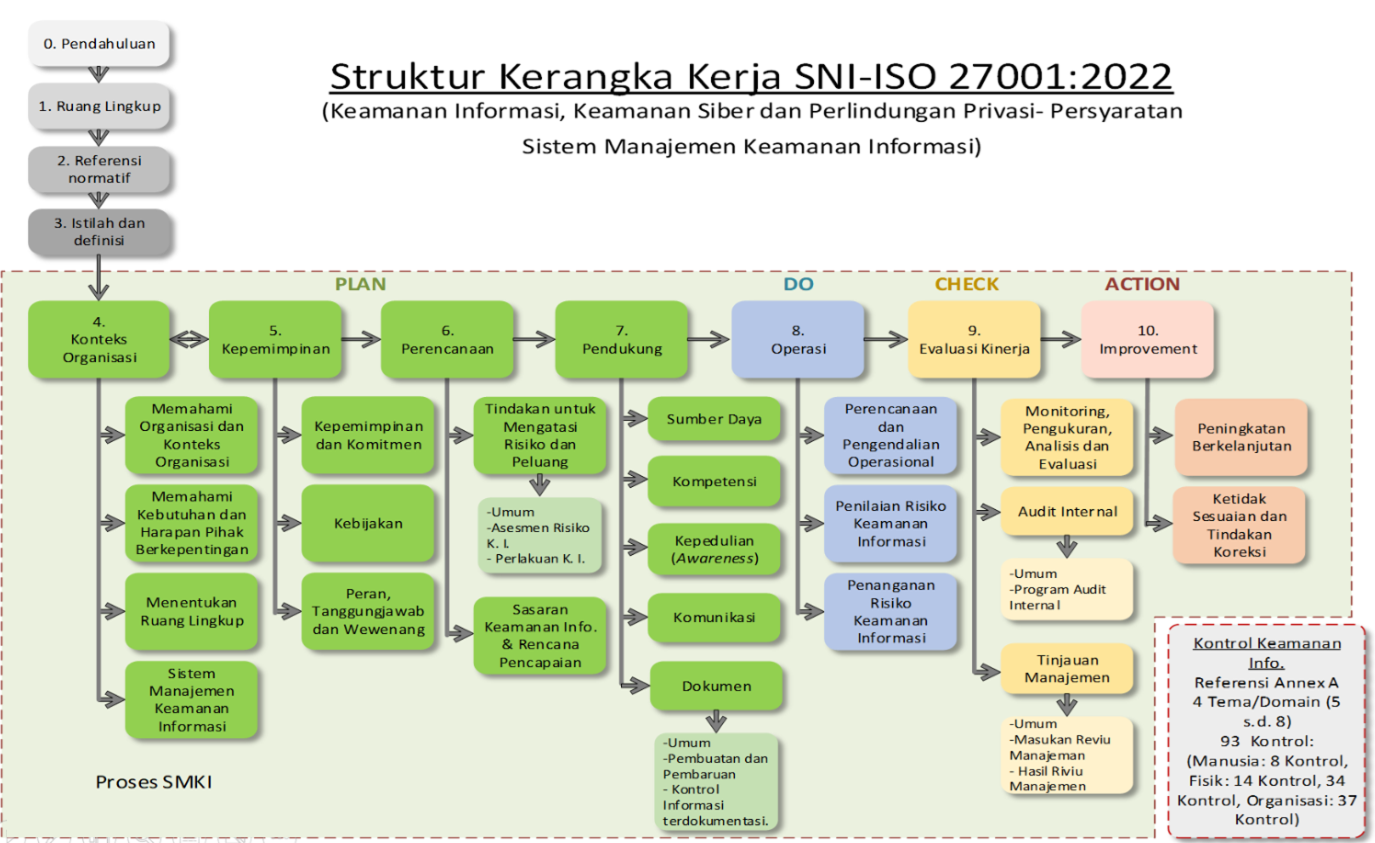
\includegraphics[width=0.9\textwidth]{Gambar/2.1Clause.png}
	\caption{Struktur klausul ISO/IEC 27001:2022 \cite{kajianAuditDataCenter2023}}
	\label{fig:iso27001_struktur}
\end{figure}

\subsection{Siklus \textit{Plan, Do, Check, Act} dalam ISO 27001}

Konsep \textit{Plan--Do--Check--Act} (PDCA) merupakan suatu siklus manajemen yang digunakan untuk mendukung perbaikan berkelanjutan dalam berbagai domain, termasuk tata kelola TI, manajemen risiko, audit, dan keamanan informasi. Model ini secara umum dikaitkan dengan W. Edwards Deming dan dikenal sebagai pendekatan iteratif yang terdiri dari empat tahapan utama untuk mengelola dan meningkatkan proses secara sistematis.

Dalam konteks ISO/IEC 27001, siklus PDCA digunakan sebagai kerangka kerja dalam pengelolaan \textit{Information Security Management System} (ISMS). Standar ini mengadopsi PDCA sebagai \textit{lifecycle} yang mencakup tahap \textit{Plan} (perencanaan), \textit{Do} (pelaksanaan dan pengoperasian), \textit{Check} (pemantauan dan peninjauan), serta \textit{Act} (pemeliharaan dan peningkatan) dalam pengelolaan keamanan informasi \cite{gantz2014itaudit}. Pendekatan ini menunjukkan bahwa ISMS tidak bersifat statis, melainkan merupakan sistem yang terus berkembang melalui proses evaluasi dan peningkatan berkelanjutan:

\begin{enumerate}
	\item \textbf{\textit{Plan}}

	Organisasi melakukan proses \textit{risk assessment} dan \textit{risk treatment planning} untuk mengidentifikasi ancaman, kerentanan, serta menentukan kontrol yang sesuai. Proses ini mencakup penentuan ruang lingkup ISMS, kebijakan keamanan informasi, serta pemilihan kontrol yang mengacu pada Annex A.

	\item \textbf{\textit{Do}}

	ISO 27001 mencakup implementasi kontrol keamanan informasi yang telah direncanakan. Implementasi ini dapat berupa penerapan kebijakan akses, pengamanan jaringan, pelatihan kesadaran keamanan (\textit{security awareness}), serta prosedur operasional lainnya yang mendukung perlindungan aset informasi. Keberhasilan tahap ini sangat bergantung pada konsistensi pelaksanaan serta keterlibatan seluruh pemangku kepentingan dalam organisasi.

	\item \textbf{\textit{Check}}

	Kegiatan \textit{monitoring} dan evaluasi terhadap efektivitas kontrol yang telah diterapkan. Aktivitas ini meliputi \textit{internal audit}, \textit{management review}, serta pengukuran kinerja keamanan informasi berdasarkan indikator yang telah ditentukan. Tujuan utama tahap ini adalah untuk memastikan bahwa implementasi ISMS berjalan sesuai dengan kebijakan dan tujuan yang telah ditetapkan.

	\item \textbf{\textit{Act}}

	Perbaikan berkelanjutan terhadap sistem manajemen keamanan informasi. Organisasi melakukan tindakan korektif terhadap temuan audit, memperbaiki kelemahan kontrol, serta menyesuaikan kebijakan dan prosedur berdasarkan perubahan lingkungan bisnis maupun ancaman keamanan yang berkembang. Dengan demikian, siklus PDCA tidak hanya memastikan kepatuhan terhadap standar, tetapi juga meningkatkan ketahanan sistem terhadap risiko keamanan informasi.
\end{enumerate}

\begin{figure}[!htbp]
	\centering
	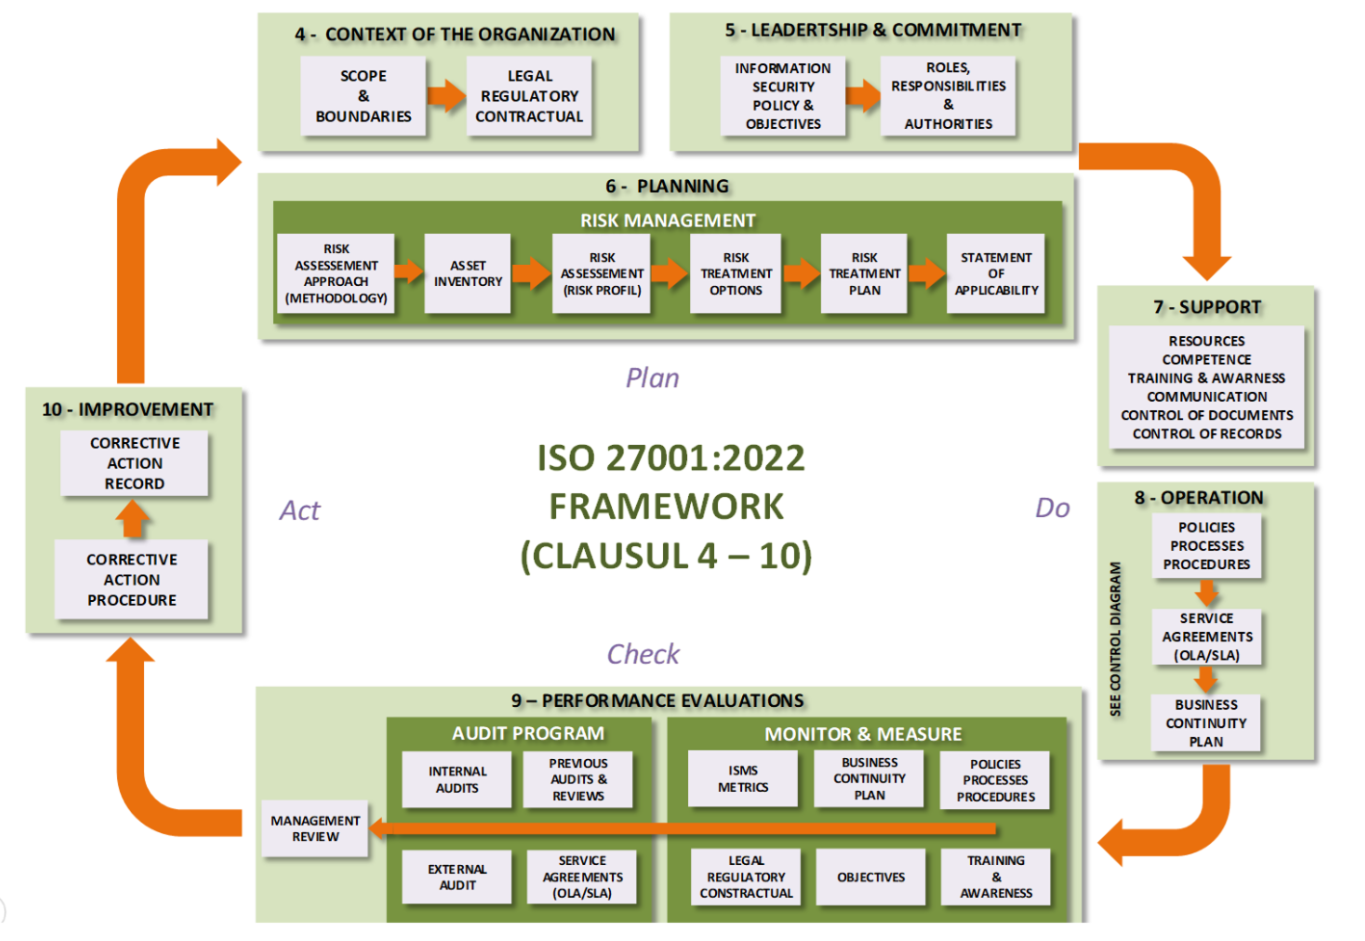
\includegraphics[width=0.85\textwidth]{Gambar/2.2PDCA.png}
	\caption{Siklus PDCA dalam ISMS \cite{kajianAuditDataCenter2023}}
	\label{fig:pdca_isms}
\end{figure}

\subsection{\textit{Statement of Applicability} (SoA)}

\textit{Statement of Applicability} (SoA) merupakan salah satu dokumen inti dalam penerapan ISO/IEC 27001 yang berfungsi untuk mendefinisikan kontrol keamanan informasi yang relevan bagi organisasi. SoA berisi daftar kontrol yang dipilih dari Annex A, disertai dengan justifikasi apakah kontrol tersebut diterapkan (\textit{applicable}) atau tidak (\textit{not applicable}), serta alasan yang mendasarinya. Dengan demikian, SoA menjadi representasi formal dari keputusan organisasi dalam mengelola risiko keamanan informasi berdasarkan hasil \textit{risk assessment} dan \textit{risk treatment}.

Dalam konteks siklus \textit{Plan--Do--Check--Act} (PDCA), SoA terutama muncul pada tahap \textit{Plan}. Pada fase ini, organisasi melakukan identifikasi risiko serta menentukan strategi penanganannya (\textit{risk treatment plan}). SoA berperan sebagai artefak yang menghubungkan hasil analisis risiko dengan pemilihan kontrol yang sesuai. Selain itu, SoA juga memiliki keterkaitan dengan tahap \textit{Do} (sebagai acuan implementasi kontrol) dan \textit{Check} (sebagai referensi dalam audit), namun fungsi utamanya tetap berada pada fase perencanaan. Oleh karena itu, SoA dapat dipandang sebagai jembatan antara proses analisis risiko dan implementasi kontrol dalam siklus ISMS.

Lebih lanjut, SoA memiliki hubungan erat dengan praktik pengendalian dokumentasi dalam ISMS, khususnya terkait \textit{control of documents} dan \textit{control of records}. Sebagai dokumen formal, SoA harus dikelola secara sistematis, termasuk dalam hal versi, otorisasi, distribusi, serta penyimpanan. Hal ini penting untuk memastikan bahwa setiap perubahan pada kontrol keamanan dapat dilacak (\textit{traceable}) dan diaudit. Selain itu, SoA juga berfungsi sebagai dokumen pemetaan (\textit{mapping document}) yang menghubungkan risiko, kontrol yang dipilih, serta status implementasinya sebelum dituangkan lebih lanjut dalam \textit{risk treatment plan}. Dengan kata lain, SoA menyediakan transparansi dan akuntabilitas dalam proses pengambilan keputusan terkait keamanan informasi.

Secara struktural, SoA umumnya disajikan dalam bentuk tabel yang terdiri dari beberapa kolom utama:

\begin{enumerate}
	\item \textbf{\textit{Control ID}} yang merujuk pada identifikasi unik setiap kontrol berdasarkan Annex A ISO/IEC 27001. Kolom ini memudahkan proses referensi dan pelacakan kontrol dalam standar.
	\item \textbf{\textit{Control Description}} yang berisi penjelasan singkat mengenai tujuan dan ruang lingkup kontrol tersebut. Kolom ini memberikan konteks bagi organisasi dalam memahami fungsi kontrol yang dipilih.
	\item \textbf{\textit{Applicability}} yang menunjukkan apakah suatu kontrol diterapkan atau tidak. Penentuan ini didasarkan pada hasil analisis risiko serta relevansi kontrol terhadap konteks organisasi.
	\item \textbf{\textit{Justification}} menjelaskan alasan di balik keputusan tersebut, baik untuk kontrol yang diterapkan maupun yang tidak. Justifikasi ini penting untuk menunjukkan bahwa keputusan yang diambil bersifat rasional dan berbasis risiko, bukan arbitrer.
	\item \textbf{\textit{Implementation Status}} yang menggambarkan tingkat implementasi kontrol, misalnya \textit{implemented}, \textit{partially implemented}, atau \textit{not implemented}.
	\item \textbf{\textit{Related Documents}} yang mengaitkan kontrol dengan kebijakan, prosedur, atau dokumen pendukung lainnya dalam organisasi.
\end{enumerate}

\subsection{Annex A ISO/IEC 27001:2022}

Annex A dalam ISO/IEC 27001:2022 berfungsi sebagai kumpulan kontrol keamanan (\textit{security controls}) yang digunakan sebagai referensi dalam proses mitigasi risiko pada \textit{Information Security Management System} (ISMS). Kontrol-kontrol ini tidak bersifat wajib untuk seluruhnya diterapkan, melainkan dipilih berdasarkan hasil \textit{risk assessment} dan \textit{risk treatment} yang dilakukan organisasi. Dengan demikian, Annex A menyediakan daftar kontrol yang terstandarisasi untuk membantu organisasi dalam menentukan langkah perlindungan yang relevan terhadap aset informasi. Pemilihan kontrol dari Annex A kemudian didokumentasikan dalam \textit{Statement of Applicability} (SoA), sehingga Annex A berperan sebagai sumber kontrol, sementara SoA menjadi artefak implementasi yang mencerminkan keputusan organisasi dalam konteks manajemen risiko.

\vspace{4pt}
\noindent\textbf{1. A.5 \textit{Organizational Controls}}

Annex A.5 berfokus pada kontrol yang berkaitan dengan aspek organisasi dan tata kelola keamanan informasi. Kontrol dalam kategori ini mencakup kebijakan, struktur organisasi, pengelolaan risiko, serta hubungan dengan pihak eksternal. Tujuan utama dari kontrol A.5 adalah memastikan bahwa keamanan informasi dikelola secara strategis dan terintegrasi dalam proses bisnis organisasi.

\begin{longtable}{|P{1.7cm}|P{5.2cm}|P{6.6cm}|}
\caption{Kontrol Annex A.5 -- \textit{Organizational Controls}}
\label{tab:annex_a5} \\
\hline
\textbf{Annex ID} & \textbf{Nama Kontrol} & \textbf{Penjelasan Singkat} \\
\hline
\endfirsthead
\hline
\textbf{Annex ID} & \textbf{Nama Kontrol} & \textbf{Penjelasan Singkat} \\
\hline
\endhead
\hline
\endfoot
A.5.1  & \textit{Policies for Information Security}                              & Menetapkan kebijakan keamanan sebagai dasar ISMS \\
\hline
A.5.2  & \textit{Information Security Roles and Responsibilities}                & Mendefinisikan peran dan tanggung jawab keamanan \\
\hline
A.5.3  & \textit{Segregation of Duties}                                          & Memisahkan fungsi untuk mencegah konflik kepentingan \\
\hline
A.5.4  & \textit{Management Responsibilities}                                    & Menetapkan akuntabilitas manajemen terhadap keamanan informasi \\
\hline
A.5.5  & \textit{Contact with Authorities}                                       & Menjalin koordinasi dengan otoritas keamanan terkait \\
\hline
A.5.6  & \textit{Contact with Special Interest Groups}                           & Berpartisipasi dalam komunitas dan forum keamanan \\
\hline
A.5.7  & \textit{Threat Intelligence}                                            & Mengelola dan menganalisis informasi ancaman keamanan \\
\hline
A.5.8  & \textit{Information Security in Project Management}                     & Mengintegrasikan kontrol keamanan dalam manajemen proyek \\
\hline
A.5.9  & \textit{Inventory of Information and Other Associated Assets}           & Mengelola inventaris aset informasi secara terstruktur \\
\hline
A.5.10 & \textit{Acceptable Use of Information and Assets}                       & Mengatur penggunaan aset sesuai kebijakan organisasi \\
\hline
A.5.11 & \textit{Return of Assets}                                               & Mengelola pengembalian aset setelah masa penggunaan \\
\hline
A.5.12 & \textit{Classification of Information}                                  & Mengklasifikasikan informasi berdasarkan tingkat sensitivitasnya \\
\hline
A.5.13 & \textit{Labelling of Information}                                       & Memberikan label informasi sesuai klasifikasi keamanan \\
\hline
A.5.14 & \textit{Information Transfer}                                           & Mengatur mekanisme transfer informasi secara aman \\
\hline
A.5.15 & \textit{Access Control}                                                 & Menetapkan kebijakan dan mekanisme pengendalian akses \\
\hline
A.5.16 & \textit{Identity Management}                                            & Mengelola identitas pengguna dalam sistem organisasi \\
\hline
A.5.17 & \textit{Authentication Information}                                     & Mengelola kredensial dan informasi autentikasi pengguna \\
\hline
A.5.18 & \textit{Access Rights}                                                  & Mengatur dan memonitor hak akses pengguna \\
\hline
A.5.19 & \textit{Information Security in Supplier Relationships}                 & Mengelola risiko keamanan dalam hubungan pemasok \\
\hline
A.5.20 & \textit{Addressing Information Security within Supplier Agreements}     & Mengintegrasikan keamanan dalam perjanjian dengan \textit{supplier} \\
\hline
A.5.21 & \textit{Managing Information Security in ICT Supply Chain}              & Mengelola keamanan dalam rantai pasok teknologi informasi \\
\hline
A.5.22 & \textit{Monitoring, Review and Change Management of Supplier Services}  & Memantau dan mengevaluasi layanan yang diberikan \textit{supplier} \\
\hline
A.5.23 & \textit{Information Security for Use of Cloud Services}                 & Mengatur kontrol keamanan dalam penggunaan layanan \textit{cloud} \\
\hline
A.5.24 & \textit{Information Security Incident Management Planning and Preparation} & Menyusun rencana penanganan insiden keamanan informasi \\
\hline
A.5.25 & \textit{Assessment and Decision on Information Security Events}         & Melakukan evaluasi terhadap kejadian keamanan informasi \\
\hline
A.5.26 & \textit{Response to Information Security Incidents}                     & Menangani insiden keamanan secara efektif dan terstruktur \\
\hline
A.5.27 & \textit{Learning from Information Security Incidents}                   & Mengambil pembelajaran dari insiden keamanan sebelumnya \\
\hline
A.5.28 & \textit{Collection of Evidence}                                         & Mengumpulkan dan mengelola bukti insiden keamanan \\
\hline
A.5.29 & \textit{Information Security During Disruption}                         & Menjaga keamanan informasi selama kondisi gangguan \\
\hline
A.5.30 & \textit{ICT Readiness for Business Continuity}                          & Menjamin kesiapan ICT untuk kelangsungan bisnis \\
\hline
A.5.31 & \textit{Legal, Statutory, Regulatory and Contractual Requirements}      & Memastikan kepatuhan terhadap regulasi dan hukum \\
\hline
A.5.32 & \textit{Intellectual Property Rights}                                   & Melindungi hak kekayaan intelektual organisasi \\
\hline
A.5.33 & \textit{Protection of Records}                                          & Menjaga keamanan dan integritas catatan organisasi \\
\hline
A.5.34 & \textit{Privacy and Protection of PII}                                  & Melindungi data pribadi dan informasi sensitif \\
\hline
A.5.35 & \textit{Independent Review of Information Security}                     & Melakukan audit independen terhadap keamanan informasi \\
\hline
A.5.36 & \textit{Compliance with Policies and Standards for Information Security} & Memastikan kepatuhan terhadap kebijakan dan standar \\
\hline
A.5.37 & \textit{Documented Operating Procedures}                                & Menyusun prosedur operasional yang terdokumentasi dengan baik \\
\hline
\end{longtable}

\vspace{4pt}
\noindent\textbf{2. A.6 \textit{People Controls}}

Annex A.6 berfokus pada aspek sumber daya manusia dalam keamanan informasi. Kontrol ini mencakup pengelolaan keamanan sebelum, selama, dan setelah masa kerja karyawan, dengan tujuan meminimalkan risiko yang berasal dari faktor manusia.

\begin{table}[!htbp]
\centering
\caption{Kontrol Annex A.6 -- \textit{People Controls}}
\label{tab:annex_a6}
\begin{tabular}{|p{1.7cm}|p{5.2cm}|p{6.6cm}|}
\hline
\textbf{Annex ID} & \textbf{Nama Kontrol} & \textbf{Penjelasan Singkat} \\
\hline
A.6.1 & \textit{Screening}                                                    & Melakukan verifikasi latar belakang calon karyawan \\
\hline
A.6.2 & \textit{Terms and Conditions of Employment}                           & Menetapkan ketentuan kerja terkait keamanan informasi \\
\hline
A.6.3 & \textit{Information Security Awareness, Education and Training}       & Menyelenggarakan pelatihan dan kesadaran keamanan informasi \\
\hline
A.6.4 & \textit{Disciplinary Process}                                         & Menerapkan mekanisme disiplin terhadap pelanggaran keamanan \\
\hline
A.6.5 & \textit{Responsibilities After Termination}                           & Menetapkan tanggung jawab pasca pemutusan hubungan kerja \\
\hline
A.6.6 & \textit{Confidentiality or Non-disclosure Agreements}                 & Mengatur perjanjian kerahasiaan untuk perlindungan informasi \\
\hline
A.6.7 & \textit{Remote Working}                                               & Mengamankan aktivitas kerja jarak jauh karyawan \\
\hline
A.6.8 & \textit{Information Security Event Reporting}                         & Mendorong pelaporan insiden keamanan oleh karyawan \\
\hline
\end{tabular}
\end{table}

\vspace{4pt}
\noindent\textbf{3. A.7 \textit{Physical Controls}}

Annex A.7 mencakup kontrol yang berfokus pada perlindungan fisik terhadap aset informasi dan fasilitas organisasi. Tujuannya adalah mencegah akses fisik yang tidak sah, kerusakan, atau gangguan terhadap infrastruktur.

\begin{table}[!htbp]
\centering
\caption{Kontrol Annex A.7 -- \textit{Physical Controls}}
\label{tab:annex_a7}
\begin{tabular}{|p{1.7cm}|p{5.2cm}|p{6.6cm}|}
\hline
\textbf{Annex ID} & \textbf{Nama Kontrol} & \textbf{Penjelasan Singkat} \\
\hline
A.7.1  & \textit{Physical Security Perimeters}                          & Menetapkan batas dan perimeter keamanan fisik \\
\hline
A.7.2  & \textit{Physical Entry Controls}                               & Mengendalikan akses masuk ke area fisik terbatas \\
\hline
A.7.3  & \textit{Securing Offices, Rooms and Facilities}                & Mengamankan ruang kerja dan fasilitas operasional \\
\hline
A.7.4  & \textit{Physical Security Monitoring}                          & Melakukan pemantauan aktivitas pada area fisik \\
\hline
A.7.5  & \textit{Protecting Against Physical and Environmental Threats}  & Melindungi aset dari ancaman fisik dan lingkungan \\
\hline
A.7.6  & \textit{Working in Secure Areas}                               & Mengatur prosedur kerja di area dengan keamanan tinggi \\
\hline
A.7.7  & \textit{Clear Desk and Clear Screen}                           & Menerapkan kebijakan meja bersih dan layar bersih \\
\hline
A.7.8  & \textit{Equipment Siting and Protection}                       & Menentukan penempatan perangkat secara aman dan terkendali \\
\hline
A.7.9  & \textit{Security of Assets Off-premises}                       & Menjaga keamanan aset saat digunakan di luar lokasi \\
\hline
A.7.10 & \textit{Storage Media}                                         & Mengelola media penyimpanan secara aman dan terkendali \\
\hline
A.7.11 & \textit{Supporting Utilities}                                  & Menjamin keamanan utilitas pendukung sistem informasi \\
\hline
A.7.12 & \textit{Cabling Security}                                      & Melindungi infrastruktur kabel dari gangguan dan kerusakan \\
\hline
A.7.13 & \textit{Equipment Maintenance}                                 & Melakukan pemeliharaan perangkat secara berkala dan aman \\
\hline
A.7.14 & \textit{Secure Disposal or Reuse of Equipment}                 & Mengelola penghapusan atau penggunaan ulang perangkat dengan aman \\
\hline
\end{tabular}
\end{table}

\vspace{4pt}
\noindent\textbf{4. A.8 \textit{Technological Controls}}

Annex A.8 berfokus pada kontrol teknis yang diterapkan pada sistem informasi, jaringan, dan aplikasi. Kontrol ini bertujuan untuk melindungi sistem dari ancaman siber serta memastikan keamanan operasional teknologi.

{\setlength{\parskip}{0pt}\setlength{\parfillskip}{0pt plus 1fil}%
\begin{longtable}{|P{1.7cm}|P{5.2cm}|P{6.6cm}|}
\caption{Kontrol Annex A.8 -- \textit{Technological Controls}}
\label{tab:annex_a8} \\
\hline
\textbf{Annex ID} & \textbf{Nama Kontrol} & \textbf{Penjelasan Singkat} \\
\hline
\endfirsthead
\hline
\textbf{Annex ID} & \textbf{Nama Kontrol} & \textbf{Penjelasan Singkat} \\
\hline
\endhead
\hline
\endfoot
A.8.1  & \textit{User Endpoint Devices}                                        & Mengamankan perangkat \textit{endpoint} pengguna dari ancaman \\
\hline
A.8.2  & \textit{Privileged Access Rights}                                     & Mengelola hak akses istimewa secara ketat \\
\hline
A.8.3  & \textit{Information Access Restriction}                               & Membatasi akses informasi sesuai kebutuhan pengguna \\
\hline
A.8.4  & \textit{Access to Source Code}                                        & Melindungi akses terhadap kode sumber aplikasi \\
\hline
A.8.5  & \textit{Secure Authentication}                                        & Menerapkan mekanisme autentikasi yang aman \\
\hline
A.8.6  & \textit{Capacity Management}                                          & Mengelola kapasitas sistem untuk menjaga kinerja \\
\hline
A.8.7  & \textit{Protection Against Malware}                                   & Melindungi sistem dari serangan perangkat lunak berbahaya \\
\hline
A.8.8  & \textit{Management of Technical Vulnerabilities}                      & Mengidentifikasi dan menangani kerentanan teknis sistem \\
\hline
A.8.9  & \textit{Configuration Management}                                     & Mengelola konfigurasi sistem secara konsisten dan aman \\
\hline
A.8.10 & \textit{Information Deletion}                                         & Menghapus informasi secara aman dan permanen \\
\hline
A.8.11 & \textit{Data Masking}                                                 & Melindungi data sensitif melalui teknik \textit{masking} \\
\hline
A.8.12 & \textit{Data Leakage Prevention}                                      & Mencegah kebocoran data melalui kontrol keamanan \\
\hline
A.8.13 & \textit{Information Backup}                                           & Melakukan pencadangan data secara berkala dan aman \\
\hline
A.8.14 & \textit{Redundancy of Information Processing Facilities}              & Menyediakan redundansi untuk menjaga ketersediaan sistem \\
\hline
A.8.15 & \textit{Logging}                                                      & Mencatat aktivitas sistem untuk keperluan audit \\
\hline
A.8.16 & \textit{Monitoring Activities}                                        & Memantau aktivitas sistem secara berkelanjutan \\
\hline
A.8.17 & \textit{Clock Synchronisation}                                        & Menyelaraskan waktu sistem untuk konsistensi \textit{log} \\
\hline
A.8.18 & \textit{Use of Privileged Utility Programs}                           & Mengontrol penggunaan program utilitas khusus \\
\hline
A.8.19 & \textit{Installation of Software on Operational Systems}              & Mengatur instalasi perangkat lunak pada sistem operasional \\
\hline
A.8.20 & \textit{Network Security}                                             & Mengamankan jaringan dari ancaman dan serangan \\
\hline
A.8.21 & \textit{Security of Network Services}                                 & Melindungi layanan jaringan yang digunakan organisasi \\
\hline
A.8.22 & \textit{Segregation of Networks}                                      & Memisahkan jaringan untuk mengurangi risiko akses \\
\hline
A.8.23 & \textit{Web Filtering}                                                & Menyaring akses \textit{web} untuk mencegah konten berbahaya \\
\hline
A.8.24 & \textit{Use of Cryptography}                                          & Menggunakan kriptografi untuk melindungi informasi sensitif \\
\hline
A.8.25 & \textit{Secure Development Life Cycle}                                & Menerapkan siklus pengembangan sistem yang aman \\
\hline
A.8.26 & \textit{Application Security Requirements}                            & Menetapkan kebutuhan keamanan pada aplikasi \\
\hline
A.8.27 & \textit{Secure System Architecture}                                   & Merancang arsitektur sistem yang aman dan andal \\
\hline
A.8.28 & \textit{Secure Coding}                                                & Menerapkan praktik pengkodean yang aman \\
\hline
A.8.29 & \textit{Security Testing in Development}                              & Melakukan pengujian keamanan selama pengembangan \\
\hline
A.8.30 & \textit{Outsourced Development}                                       & Mengelola keamanan dalam pengembangan oleh pihak ketiga \\
\hline
A.8.31 & \textit{Separation of Development, Test and Production Environments}  & Memisahkan lingkungan pengembangan, uji, dan produksi \\
\hline
A.8.32 & \textit{Change Management}                                            & Mengelola perubahan sistem secara terkontrol \\
\hline
A.8.33 & \textit{Test Information}                                             & Mengelola data uji agar tetap aman \\
\hline
A.8.34 & \textit{Protection of Information Systems During Audit Testing}       & Melindungi sistem saat proses audit dan pengujian \\
\hline
\end{longtable}
}

\subsection{Keterbatasan Pendekatan Konvensional dalam Audit Keamanan Informasi}

Meskipun kerangka ISO/IEC 27001:2022 dan ISMS telah menyediakan pendekatan sistematis, proses audit masih menghadapi kendala pada analisis dan penelusuran bukti. Auditor umumnya mengaitkan temuan dengan kontrol dan regulasi secara manual, yang bergantung pada pengetahuan individu sehingga membatasi efisiensi dan konsistensi. Di sisi lain, besarnya volume dokumen audit membuat proses menjadi memakan waktu, rentan kesalahan, dan berpotensi menimbulkan inkonsistensi \cite{auditgpt2025}.

Perkembangan \textit{Natural Language Processing} melalui \textit{Large Language Models} menawarkan otomasi analisis dokumen, namun masih memiliki keterbatasan seperti kurangnya \textit{grounding} terhadap data spesifik. Oleh karena itu, \textit{Retrieval-Augmented Generation} menjadi pendekatan yang lebih andal dengan menggabungkan kemampuan generatif dan \textit{retrieval} berbasis dokumen untuk meningkatkan akurasi dan konsistensi dalam proses audit \cite{lajbr2025}.

\subsection{\textit{Natural Language Processing}}

Pemrosesan bahasa alami (\textit{natural language processing}, NLP) merupakan bagian dari kecerdasan buatan yang memungkinkan komputer untuk memahami dan menghasilkan bahasa manusia. NLP terdiri dari dua komponen utama, yaitu \textit{natural language understanding} (NLU) dan \textit{natural language generation} (NLG). NLU berfokus pada kemampuan sistem dalam memahami makna dari bahasa yang digunakan manusia, termasuk menangani konteks, ambiguitas, serta berbagai bentuk ekspresi bahasa. Sementara itu, NLG bertugas untuk menghasilkan teks yang menyerupai bahasa manusia, melalui proses pemilihan informasi yang relevan, penyusunan isi, serta pengaturan struktur dan gaya bahasa agar mudah dipahami \cite{pajila2023nlp}.

\subsection{\textit{Transformer}}

Arsitektur \textit{Transformer} merupakan model yang diperkenalkan oleh Vaswani et al. melalui publikasi berjudul \textit{``Attention Is All You Need''} \cite{vaswani2017attention}. Model ini menghadirkan pendekatan baru dalam pemodelan tugas NLP. Sebelum adanya \textit{Transformer}, berbagai tugas sekuensial umumnya mengandalkan arsitektur \textit{Recurrent Neural Network} (RNN) dan \textit{Convolutional Neural Network} (CNN). Kedua arsitektur tersebut memiliki kekurangan yaitu memproses data harus secara berurutan menyebabkan keterbatasan dalam efisiensi pelatihan serta kesulitan dalam menangkap hubungan konteks jangka panjang antar elemen dalam data.

Sebagai solusi, \textit{Transformer} dirancang tanpa bergantung pada mekanisme RNN maupun CNN, melainkan mengandalkan mekanisme \textit{attention}, khususnya \textit{self-attention}. Mekanisme ini memungkinkan model untuk mengevaluasi keterkaitan antar kata dalam suatu urutan secara lebih fleksibel, sehingga mampu memahami konteks secara menyeluruh dan menghasilkan representasi yang lebih baik. Secara teknis, struktur arsitektur \textit{Transformer}, khususnya bagian \textit{encoder} umumnya disajikan dalam bentuk diagram untuk menggambarkan alur pemrosesannya (Gambar~\ref{fig:transformer}).

\begin{figure}[!htbp]
	\centering
	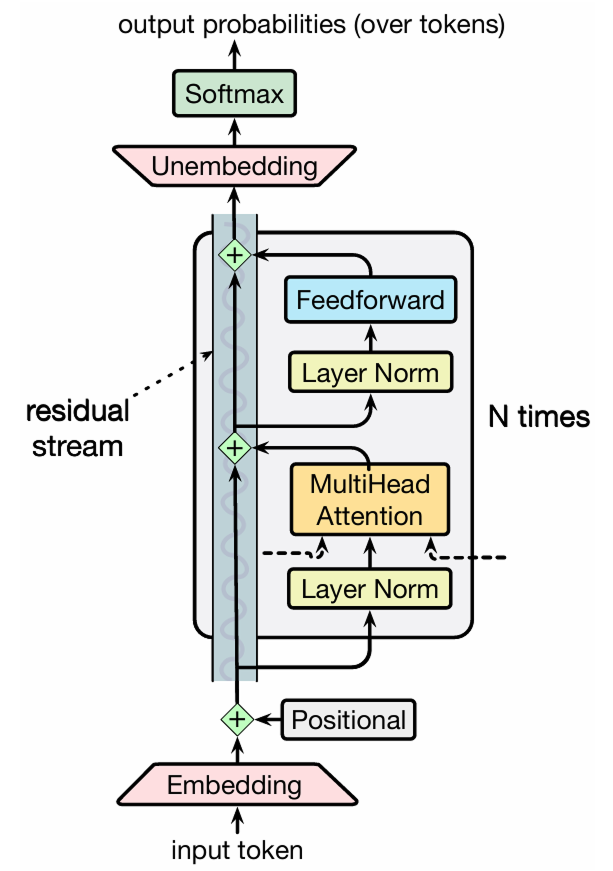
\includegraphics[width=0.42\textwidth,height=0.38\textheight,keepaspectratio]{Gambar/2.3Transformer.png}
	\caption{Arsitektur Transformer \cite{jurafsky2026slp}}
	\label{fig:transformer}
\end{figure}

Arsitektur ini terdiri dari beberapa komponen utama yang bekerja secara terintegrasi dalam memproses dan menghasilkan teks:

\begin{enumerate}
	\item \textbf{\textit{Embedding}} dan \textbf{\textit{Unembedding}} berfungsi untuk mengubah token menjadi representasi vektor serta memetakan kembali representasi tersebut ke ruang kosakata untuk menghasilkan prediksi kata berikutnya \cite{jurafsky2026slp}.
	\item \textbf{\textit{Positional Encoding}} ditambahkan ke \textit{embedding} untuk mempertahankan informasi urutan token dalam suatu kalimat.
	\item \textbf{\textit{Layer Normalization}} digunakan untuk menstabilkan proses pelatihan dengan menjaga nilai dalam \textit{layer} tetap berada pada rentang yang mendukung optimasi berbasis gradien.
	\item \textbf{\textit{Multi-head Attention}} merupakan mekanisme inti yang memungkinkan model menangkap hubungan kontekstual antar token melalui proses \textit{query}, \textit{key}, dan \textit{value} secara paralel.
	\item \textbf{\textit{Feedforward Network}} berfungsi sebagai transformasi non-linear yang diterapkan pada setiap token untuk memperkaya representasi fitur.
	\item \textbf{\textit{Softmax}} digunakan untuk mengubah \textit{output} model menjadi distribusi probabilitas atas seluruh kosakata, sehingga memungkinkan pemilihan token berikutnya secara probabilistik.
\end{enumerate}

\subsection{\textit{Large Language Model}}

\textit{Large Language Models} (LLM) merupakan model \textit{machine learning} dalam bidang \textit{natural language processing} yang dirancang untuk memahami dan menghasilkan teks dengan mempelajari pola statistik dari data berskala besar. Secara umum, model bahasa bekerja dengan memprediksi kata berikutnya dalam suatu urutan serta menghasilkan distribusi probabilitas atas kemungkinan kata yang dapat muncul. Pendekatan ini memungkinkan model untuk mempelajari struktur linguistik, makna, serta hubungan kontekstual antar kata dari data pelatihan. Perkembangan LLM modern yang berbasis arsitektur \textit{transformer} mampu menangkap konteks secara lebih luas dan kompleks \cite{jurafsky2026slp}.

Dengan kapasitas pengetahuan yang besar serta mekanisme pemrosesan yang kompleks, LLM mampu menjalankan berbagai tugas berbasis bahasa, seperti menghasilkan teks, merangkum dokumen, menjawab pertanyaan, menghasilkan kode program, hingga melakukan penalaran secara bertahap \cite{mienye2025llm,shao2024llmsurvey}. Kemampuan ini memungkinkan LLM untuk diterapkan pada berbagai domain yang memerlukan pemahaman spesifik. Sebagai contoh, dalam bidang hukum, LLM dimanfaatkan untuk mendukung pekerjaan profesional, seperti penyusunan dokumen, analisis kontrak, serta proses uji tuntas yang umumnya memerlukan waktu dan tenaga yang signifikan \cite{katz2024gpt4bar}.

\subsection{\textit{Prompt Engineering}}

Tidak seperti \textit{fine-tuning} yang membutuhkan \textit{training} parameter model, \textit{prompt engineering} berfokus pada penyusunan instruksi berbasis bahasa alami untuk menggunakan pengetahuan yang telah dipelajari oleh model \textit{pre-trained} \cite{vatsal2024prompt}. Tujuan utama dari teknik ini adalah mengontrol dan memberi arahan respons LLM secara spesifik, mengurangi ambiguitas konteks, serta menjaga relevansi jawaban tanpa perlu mengubah struktur maupun parameter model, sehingga dapat diterapkan pada berbagai kebutuhan domain spesifik \cite{chaubey2024ragcompare,chen2024prompt}.

\subsection{\textit{Information Retrieval}}

\textit{Information Retrieval} (IR) merupakan bidang yang berfokus pada proses pencarian dan pengambilan berbagai jenis informasi berdasarkan kebutuhan pengguna, yang umumnya diimplementasikan dalam bentuk \textit{search engine}. Salah satu tugas utama dalam IR adalah \textit{ad hoc retrieval}, di mana pengguna mengajukan kueri dan sistem mengembalikan sekumpulan dokumen yang telah diurutkan berdasarkan relevansi dari suatu koleksi tertentu. Dalam konteks ini, dokumen merujuk pada unit teks yang diindeks dan diambil (seperti halaman \textit{web}, artikel ilmiah, atau paragraf) serta koleksi adalah himpunan dokumen yang digunakan untuk memenuhi kebutuhan informasi.

\begin{figure}[!htbp]
	\centering
	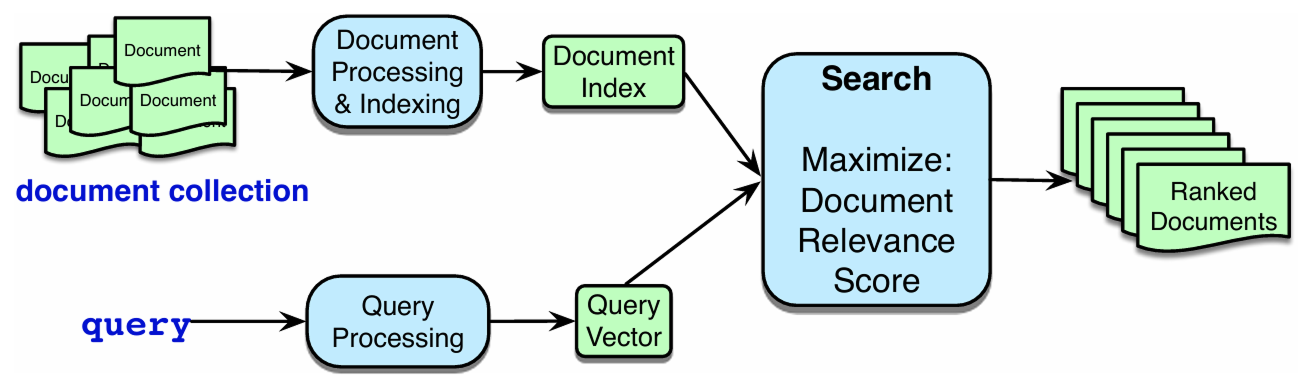
\includegraphics[width=0.9\textwidth]{Gambar/2.4IR.png}
	\caption{Arsitektur umum sistem information retrieval \cite{jurafsky2026slp}}
	\label{fig:ir_arsitektur}
\end{figure}

Arsitektur tingkat tinggi dari sistem \textit{ad hoc retrieval} terdiri dari dua pendekatan utama berdasarkan representasi vektor yang digunakan, yaitu \textit{sparse retrieval} dan \textit{dense retrieval}. Pada \textit{sparse retrieval}, dokumen dan kueri direpresentasikan sebagai vektor berbasis frekuensi kata (\textit{count vectors}) yang umumnya diberi bobot menggunakan metode seperti TF-IDF atau BM25. Sementara itu, pada \textit{dense retrieval}, dokumen dan kueri direpresentasikan dalam bentuk \textit{embedding} yang dihasilkan oleh model bahasa (baik \textit{encoder} maupun \textit{decoder}), sehingga mampu menangkap hubungan semantik yang lebih kompleks \cite{jurafsky2026slp}.

\subsection{\textit{Retrieval-Augmented Generation}}

\textit{Retrieval-Augmented Generation} (RAG) merupakan metode yang mengintegrasikan teknik \textit{information retrieval} (IR) ke dalam \textit{language model} untuk meningkatkan kualitas jawaban yang dihasilkan. Dalam skenario dasar RAG, sistem terlebih dahulu mengambil dokumen yang relevan dari suatu basis pengetahuan menggunakan teknik \textit{retrieval}, kemudian memanfaatkan \textit{large language model} (LLM) untuk menghasilkan jawaban berdasarkan dokumen tersebut serta \textit{query} pengguna \cite{jurafsky2026slp}. Pendekatan ini memiliki beberapa tujuan utama, antara lain mengurangi halusinasi dengan menyediakan sumber informasi yang tepercaya, memungkinkan pemanfaatan data spesifik atau privat (seperti dokumen internal, rekam medis, atau \textit{email}), serta mengatasi keterbatasan pengetahuan model yang bersifat statis dan tidak selalu mutakhir.

\begin{figure}[!htbp]
	\centering
	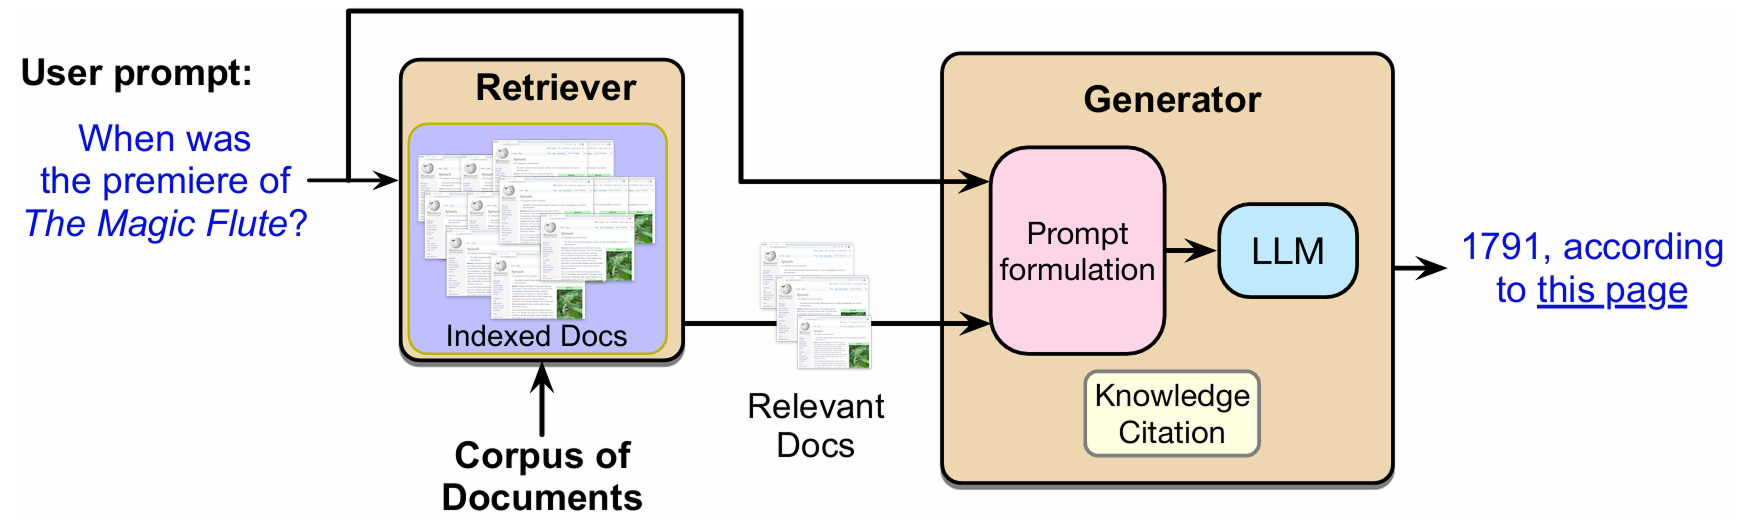
\includegraphics[width=0.9\textwidth]{Gambar/2.5RAG.png}
	\caption{Arsitektur Retrieval-Augmented Generation \cite{jurafsky2026slp}}
	\label{fig:rag_arsitektur}
\end{figure}

Secara arsitektural, RAG terdiri dari dua komponen utama, yaitu \textit{retriever} yang bertugas mengindeks dan mengambil data relevan (biasanya dalam bentuk vektor), serta \textit{generator} (LLM) yang memanfaatkan konteks tersebut untuk menghasilkan respons yang koheren dan berbasis fakta, sehingga meningkatkan keandalan dan mengurangi risiko halusinasi \cite{fan2024ragsurvey}.

\subsection{Metrik Evaluasi}

Evaluasi performa sistem \textit{Retrieval-Augmented Generation} (RAG) memerlukan metrik yang mampu mengukur kualitas hasil \textit{retrieval} serta efektivitas peringkat dokumen relevan, sekaligus mempertimbangkan efisiensi sistem dari sisi komputasi. Oleh karena itu, digunakan beberapa metrik evaluasi standar yang mencakup aspek keberhasilan \textit{retrieval}, kualitas pemeringkatan dokumen, serta efisiensi waktu respons sistem. Berikut adalah metrik-metrik yang digunakan:

\begin{enumerate}
	\item \textbf{Hit@k}

	Hit@k digunakan untuk mengukur apakah setidaknya satu dokumen relevan muncul dalam top-$k$ hasil \textit{retrieval}. Metrik ini bersifat biner (\textit{hit} atau tidak), sehingga sering digunakan untuk mengevaluasi keberhasilan minimum sistem dalam menemukan jawaban yang benar.

	\begin{equation}
		\text{Hit@}k = \frac{\text{Jumlah \textit{query} dengan} \geq 1 \text{ dokumen relevan di top-}k}{\text{Total \textit{query}}}
	\end{equation}

	dengan:
	\begin{itemize}
		\item \textit{Query} dengan $\geq 1$ dokumen relevan: jumlah \textit{query} yang memiliki minimal satu hasil relevan dalam top-$k$
		\item Total \textit{query}: jumlah seluruh \textit{query} yang diuji
	\end{itemize}

	\item \textbf{Recall@k}

	Recall@k digunakan untuk mengukur kemampuan sistem dalam menemukan dokumen relevan dalam sejumlah top-$k$ hasil \textit{retrieval}. Metrik ini berfokus pada \textit{coverage}, yaitu seberapa banyak dokumen relevan yang berhasil ditemukan dibandingkan dengan seluruh dokumen relevan yang tersedia. Recall@k sangat penting dalam konteks RAG karena menentukan apakah informasi yang dibutuhkan sudah masuk ke dalam kandidat awal sebelum tahap generasi.

	\begin{equation}
		\text{Recall@}k = \frac{\text{Total dokumen relevan}}{\text{Jumlah dokumen relevan dalam top-}k}
	\end{equation}

	dengan:
	\begin{itemize}
		\item Total dokumen relevan: seluruh dokumen yang seharusnya relevan dalam \textit{corpus}
		\item Dokumen relevan dalam top-$k$: jumlah dokumen relevan yang berhasil ditemukan dalam $k$ teratas
	\end{itemize}

	\item \textbf{Average Reciprocal Rank (ARR)}

	\textit{Average Reciprocal Rank} (ARR) digunakan untuk mengukur kualitas posisi seluruh dokumen relevan yang berhasil ditemukan sistem pada hasil \textit{retrieval}. Berbeda dengan \textit{Mean Reciprocal Rank} (MRR) yang hanya mempertimbangkan dokumen relevan pertama, ARR menghitung kontribusi \textit{ranking} dari seluruh \textit{ground truth} yang berhasil ditemukan pada top-$k$ hasil \textit{retrieval}. Metrik ini berfokus pada seberapa baik sistem menempatkan banyak dokumen relevan pada posisi atas hasil pencarian. Semakin tinggi nilai ARR, maka semakin baik kemampuan sistem dalam mengembalikan keseluruhan dokumen relevan pada \textit{ranking} yang lebih tinggi.

	\begin{equation}
		\text{ARR} = \frac{1}{|G|} \sum_{i=1}^{|G|} \frac{1}{\text{rank}_i}
	\end{equation}

	dengan:
	\begin{itemize}
		\item $|G|$ = jumlah total \textit{ground truth} unik
		\item $\text{rank}_i$ = posisi dokumen relevan pertama untuk \textit{query} ke-$i$
	\end{itemize}

	\item \textbf{Normalized Discounted Cumulative Gain (NDCG)}

	nDCG digunakan untuk mengevaluasi kualitas \textit{ranking} dengan mempertimbangkan posisi dan tingkat relevansi dokumen. Dokumen yang relevan pada posisi lebih atas akan memberikan kontribusi nilai yang lebih tinggi. Metrik ini cocok untuk skenario di mana relevansi tidak bersifat biner.

	\begin{equation}
		\text{NDCG@}k = \frac{\text{DCG@}k}{\text{IDCG@}k}
	\end{equation}

	\begin{equation}
		\text{DCG@}k = \sum_{i=1}^{k} \frac{2^{rel_i} - 1}{\log_2(i+1)}
	\end{equation}

	\begin{equation}
		\text{IDCG@}k = \sum_{i=1}^{k} \frac{2^{rel_{ideal,i}} - 1}{\log_2(i+1)}
	\end{equation}

	dengan:
	\begin{itemize}
		\item DCG@$k$: \textit{Discounted Cumulative Gain}, yaitu akumulasi skor relevansi dengan pembobotan posisi
		\item IDCG@$k$: nilai DCG ideal (\textit{ranking} terbaik)
		\item $rel_i$: skor relevansi bertingkat dari dokumen pada posisi $i$
		\item Faktor diskonto logaritmik $\log_2(i + 1)$ digunakan untuk memberi penalti pada dokumen yang berada di peringkat lebih rendah
	\end{itemize}

	\item \textbf{Latensi Waktu}

	Evaluasi sistem ketepatan \textit{Information Retrieval} pemilihan dokumen pada \textit{Information Retrieval} tidak hanya berfokus pada kualitas hasil (akurasi dan relevansi), tetapi juga pada efisiensi waktu pemrosesan. Oleh karena itu, metrik latensi digunakan untuk mengukur waktu yang dibutuhkan sistem dalam memproses satu \textit{query} hingga menentukan dokumen yang relevan. Latensi menjadi penting terutama pada sistem yang melibatkan beberapa tahapan seperti \textit{hybrid retrieval}, dan \textit{reranking}, karena setiap komponen tambahan berpotensi meningkatkan waktu eksekusi.

	\begin{equation}
		\text{Latensi}_{\text{Total}} = t_{\text{retrieval}} + t_{\text{rerank}}
	\end{equation}

	dengan:
	\begin{itemize}
		\item $t_{\text{retrieval}}$ = waktu untuk mengambil kandidat dokumen dari basis pengetahuan
		\item $t_{\text{rerank}}$ = waktu untuk melakukan pengurutan ulang hasil menggunakan \textit{reranker}
	\end{itemize}
\end{enumerate}

\section{Analisis Perbandingan Metode}

Bagian ini menyajikan analisis komparatif antara komponen metode dalam \textit{Retrieval-Augmented Generation} (RAG), yaitu \textit{hybrid retrieval} dan \textit{reranking}, serta kombinasinya. Perbandingan lengkap disajikan dalam Tabel berikut:

\begin{table}[!htbp]
\centering
\caption{Perbandingan Komponen Metode RAG}
\label{tab:komparasi_metode}
\begin{tabular}{|p{2.3cm}|p{5.8cm}|p{5.8cm}|}
\hline
\textbf{Metode} & \textbf{Kelebihan} & \textbf{Kekurangan} \\
\hline
\textit{Hybrid Retrieval} &
$\bullet$ Menggabungkan pendekatan leksikal dan semantik sehingga meningkatkan cakupan dokumen relevan (Recall@100: 0,49 $\rightarrow$ 0,60; +11\%) [Rustamov et al., 2025]. \newline
$\bullet$ Meningkatkan \textit{coverage} dibanding metode \textit{dense} tunggal [Liu et al., 2025]. \newline
$\bullet$ Lebih \textit{robust} terhadap variasi \textit{query} melalui pendekatan \textit{multi-path retrieval} [Liu et al., 2025].
&
$\bullet$ Kompleksitas implementasi lebih tinggi karena melibatkan beberapa komponen \textit{retrieval} dan mekanisme \textit{score fusion} [Ravishankar-Varalakshmi, 2025; Elkiran-Rasheed, 2026]. \newline
$\bullet$ Memerlukan penyesuaian parameter fusi skor (mis. $\alpha$) [Ravishankar-Varalakshmi, 2025]. \newline
$\bullet$ Kualitas peringkat awal belum optimal tanpa \textit{reranking} (NDCG awal 0,39) [Rustamov et al., 2025].
\\
\hline
\textit{Reranking} (\textit{Cross-Encoder}) &
$\bullet$ Meningkatkan presisi dan kualitas hasil peringkat teratas (NDCG: 0,39 $\rightarrow$ 0,44) [Rustamov et al., 2025]. \newline
$\bullet$ Menghasilkan peringkat yang lebih relevan (R@1 = 0,687; MRR = 0,725) [Elkiran-Rasheed, 2026]. \newline
$\bullet$ Meningkatkan kualitas pada metrik tertentu seperti NDCG dan \textit{correctness} [Rustamov et al., 2025; Elkiran-Rasheed, 2026]. \newline
$\bullet$ Mengurangi hasil tidak relevan (\textit{false positive} sebesar 6\%) [Gupta et al., 2025].
&
$\bullet$ Biaya komputasi lebih tinggi dibanding tahap \textit{retrieval} awal [Gupta et al., 2025; Elkiran-Rasheed, 2026]. \newline
$\bullet$ Menambah latensi (2,76--3,12 detik pada \textit{reranker}) [Elkiran-Rasheed, 2026]. \newline
$\bullet$ Kurang efisien untuk jumlah kandidat besar karena keterbatasan skala pada \textit{cross-encoder} [Gupta et al., 2025].
\\
\hline
Kombinasi (\textit{Hybrid} + \textit{Reranking}) &
$\bullet$ Mengoptimalkan \textit{recall} dan \textit{precision} secara simultan (Precision@10 = 98,2\%) [Gupta et al., 2025]. \newline
$\bullet$ Menunjukkan performa tinggi pada konfigurasi terbaik (\textit{combined score} 0,9441) [Ravishankar-Varalakshmi, 2025]. \newline
$\bullet$ Mengungguli konfigurasi parsial pada studi \textit{ablation} ($\sim$21\% peningkatan Hit dan $\sim$30\% peningkatan MRR dibanding \textit{dense-only}) [Liu et al., 2025]. \newline
$\bullet$ Adaptif terhadap variasi \textit{query} [Elkiran-Rasheed, 2026].
&
$\bullet$ Kompleksitas \textit{pipeline} paling tinggi karena melibatkan beberapa tahap (\textit{retrieval}, fusi, \textit{reranking}, dan generasi) [Ravishankar-Varalakshmi, 2025; Elkiran-Rasheed, 2026]. \newline
$\bullet$ Latensi lebih tinggi dibanding metode tunggal (sekitar 3,4 detik) [Gupta et al., 2025]. \newline
$\bullet$ Membutuhkan proses \textit{tuning} yang lebih kompleks (top-$k$, \textit{reranker}, parameter $\alpha$) [Ravishankar-Varalakshmi, 2025]. \newline
$\bullet$ Risiko penurunan efisiensi (\textit{diminishing return}) [Rustamov et al., 2025; Elkiran-Rasheed, 2026].
\\
\hline
\end{tabular}
\end{table}

Berdasarkan analisis pada Tabel tersebut, pemilihan variasi metode dalam penelitian ini didasarkan pada pertimbangan terkait kontribusi masing-masing komponen dalam meningkatkan kualitas \textit{retrieval} serta dampaknya terhadap efisiensi sistem:

\begin{enumerate}
	\item \textit{Hybrid retrieval} dipilih sebagai \textit{baseline} karena mampu meningkatkan cakupan dokumen relevan melalui kombinasi pendekatan leksikal dan semantik, serta terbukti memberikan peningkatan \textit{recall} dibanding metode tunggal.
	\item \textit{Reranking} berbasis \textit{cross-encoder} digunakan untuk meningkatkan presisi dan kualitas hasil pada peringkat teratas dengan menyaring kandidat yang kurang relevan.
	\item Kombinasi dua komponen dianalisis untuk mengevaluasi potensi peningkatan performa secara menyeluruh sekaligus mengidentifikasi \textit{trade-off} terhadap kompleksitas dan latensi sistem.
\end{enumerate}



\cleardoublepage \phantomsection
% Catatan: Pastikan paket berikut tersedia di main.tex:
%   \usepackage{multirow}    % untuk sel bertingkat pada tabel
%   \usepackage{longtable}   % untuk tabel panjang (tabel jenis query)
%   \usepackage{array}       % untuk p{} column type
%   \usepackage{booktabs}    % opsional untuk garis tabel
%
% Catatan Penomoran: Pada dokumen sumber PDF, terdapat tiga subbab
% yang sama-sama diberi nomor 3.2.2. Pada file ini, penomoran
% disesuaikan menjadi 3.2.2, 3.2.3, dan 3.2.4 oleh LaTeX secara otomatis.

%%\documentclass[../../main.tex]{subfiles} %% Uncomment for standalone compile

%%\begin{document} %% Uncomment for standalone compile

\chapter{Metode Penelitian}

Bab ini menjelaskan metodologi penelitian yang digunakan dalam pengembangan dan evaluasi sistem \textit{information retrieval} berbasis \textit{hybrid retrieval} dan \textit{cross-encoder reranking}. Pendekatan \textit{hybrid retrieval} menggabungkan metode \textit{dense} dan \textit{sparse retrieval}, kemudian dikombinasikan dengan mekanisme \textit{reranking} menggunakan \textit{cross-encoder} melalui skema pembobotan (\textit{alpha}) untuk mengoptimalkan relevansi hasil pencarian. Pembahasan dalam bab ini mencakup perancangan basis pengetahuan berbasis dokumen ISO/IEC 27001:2022, penyusunan \textit{query} dari dokumen kebijakan Direktorat Teknologi Informasi (DTI) UGM untuk kebutuhan evaluasi, implementasi metode \textit{retrieval} dan \textit{reranking}, serta perancangan skenario pengujian berdasarkan variasi parameter penelitian.

\section{Alat dan Bahan}

\subsection{Alat Tugas Akhir}

Alat-alat yang digunakan pada penelitian ini berupa perangkat keras maupun perangkat lunak sebagai sarana pendukung. Perangkat keras dan lunak yang digunakan berfungsi untuk menulis kode, pengembangan sistem, melakukan pengujian, dan pengumpulan data.

\begin{enumerate}
	\item Laptop Lenovo Ideapad Flex 5i dengan spesifikasi
	\begin{itemize}
		\item CPU: 12th Gen Intel(R) Core(TM) i7-1255U (10 cores)
		\item RAM: 16 GB (2x8GB DDR4 4267 MHz)
		\item GPU: Intel(R) Iris(R) Xe Graphics (128 MB VRAM)
		\item Penyimpanan: SSD 512 GB (INTEL SSDPEKNW512GZL)
		\item OS: Windows 11 Home Single Language (Build 22631)
	\end{itemize}

	\item Model AI
	\begin{itemize}
		\item \textit{Embedding model}: paraphrase-multilingual-MiniLM-L12-v2 (384 \textit{dimensions}, \textit{multilingual} termasuk Bahasa Indonesia)
		\item \textit{Reranking model}: BAAI/bge-reranker-v2-m3 (\textit{cross-encoder multilingual})
	\end{itemize}

	\item Perangkat Lunak
	\begin{itemize}
		\item Visual Studio Code sebagai \textit{Integrated Development Environment} (IDE) yang digunakan untuk menulis kode program, melakukan \textit{debugging}, serta mengelola proses pengembangan sistem.
		\item Python 3.11.5 sebagai bahasa pemrograman utama yang digunakan untuk mengimplementasikan seluruh komponen sistem.
		\item Git sebagai sistem kontrol versi yang digunakan untuk mengelola \textit{source code} serta melakukan pelacakan perubahan selama pengembangan.
	\end{itemize}
\end{enumerate}

\subsection{Bahan Tugas Akhir}

Dalam proses pengembangan dan evaluasi sistem \textit{Retrieval-Augmented Generation} (RAG), diperlukan beberapa bahan sebagai berikut:

\begin{enumerate}
	\item Dokumen standar ISO/IEC 27001:2022 ``INTERNATIONAL STANDARD ISO/IEC 27001 Third Edition 2022-10'' sebagai sumber utama pengetahuan yang digunakan dalam proses \textit{retrieval} dan pembentukan basis dokumen.
	\item Dokumen kebijakan dari Direktorat Teknologi Informasi (DTI) UGM berbentuk surat edaran dan surat keputusan Rektor Universitas Gadjah Mada yang digunakan sebagai sumber penyusunan \textit{query} dan \textit{ground truth} untuk evaluasi sistem.
\end{enumerate}

\section{Metode yang Digunakan}

\subsection{Desain Penelitian}

Desain penelitian disusun dengan menentukan variabel independen, dependen, dan kontrol agar proses pengujian dapat dilakukan secara sistematis dan terukur. Variabel independen mencakup tiga parameter utama yang dievaluasi secara berurutan: proporsi bobot \textit{scoring} antara \textit{dense} dan \textit{sparse}, jumlah kandidat pada tahap \textit{reranker}, serta proporsi bobot \textit{scoring} antara \textit{hybrid} dan \textit{reranker}. Setiap parameter pada tahap berikutnya menggunakan konfigurasi optimal dari tahap sebelumnya sehingga pencarian parameter bersifat sekuensial, bukan kombinatorik. Variabel dependen digunakan untuk mengukur performa sistem berdasarkan akurasi \textit{retrieval} dan waktu latensi. Sementara itu, variabel kontrol dijaga tetap konstan selama eksperimen untuk memastikan hasil pengujian lebih konsisten dan dapat dibandingkan secara objektif.



\begin{table}[H]
\centering
\small
\caption{Variabel Penelitian (Independen)}
\label{tab:variabel_penelitian}
\begin{tabular}{|p{1.8cm}|p{3.0cm}|p{4.6cm}|p{3.4cm}|}
\hline
\textbf{Jenis} & \textbf{Nama Variabel} & \textbf{Deskripsi} & \textbf{Indikator / Parameter} \\
\hline
Independen & Proporsi bobot \textit{scoring} \textit{dense}:\textit{sparse} & Rasio pembobotan skor \textit{dense retrieval} dan \textit{sparse retrieval} pada \textit{hybrid retrieval} & \begin{tabular}[t]{@{}l@{}}alpha\_dense $\in$\\$\{0{,}0;\ 0{,}25;$\\$0{,}5;\ 0{,}75;\ 1{,}0\}$\end{tabular} \\
\hline
Independen & Jumlah kandidat & Banyaknya dokumen kandidat yang diproses oleh \textit{cross-encoder reranker} & $k \in \{5;\ 10;\ 15;\ 20\}$ \\
\hline
Independen & Proporsi bobot \textit{scoring} \textit{hybrid}:\textit{reranker} & Rasio pembobotan skor \textit{hybrid retrieval} dan skor \textit{reranker} pada skor akhir & \begin{tabular}[t]{@{}l@{}}alpha\_reranker $\in$\\$\{0{,}0;\ 0{,}25;$\\$0{,}5;\ 0{,}75;\ 1{,}0\}$\end{tabular} \\
\hline
\end{tabular}
\end{table}

\begin{table}[H]
\centering
\small
\caption{Variabel Penelitian (Dependen dan Kontrol)}
\label{tab:variabel_penelitian_lanjutan}
\begin{tabular}{|p{1.8cm}|p{3.0cm}|p{4.6cm}|p{3.4cm}|}
\hline
\textbf{Jenis} & \textbf{Nama Variabel} & \textbf{Deskripsi} & \textbf{Indikator / Parameter} \\
\hline
Dependen & Akurasi \textit{Retrieval} & Tingkat relevansi hasil \textit{retrieval} terhadap \textit{ground truth} & Hit@3, Recall@3, MAP@3, NDCG@3 \\
\hline
Dependen & Latensi Sistem & Waktu yang dibutuhkan sistem dalam memproses hingga menghasilkan \textit{output} & Waktu eksekusi \\
\hline
Kontrol & Model \textit{Embedding} dan \textit{Reranker} & Model yang digunakan dijaga tetap sama untuk semua skenario & paraphrase-multilingual-MiniLM-L12-v2 dan BGE \textit{reranker} \\
\hline
Kontrol & \textit{Dataset} Penelitian & Kumpulan \textit{query} dan dokumen sumber yang digunakan pada seluruh skenario pengujian tetap sama; \textit{query} dibentuk dari dokumen DTI UGM & \textit{Query} DTI UGM beserta \textit{ground truth}, Dokumen ISO 27001:2022 \\
\hline
Kontrol & Lingkungan Sistem & Spesifikasi perangkat dan \textit{environment} eksekusi dijaga konstan & Laptop, OS, \textit{dependency} \\
\hline
\end{tabular}
\end{table}

\subsection{Pembangunan Basis Pengetahuan ISO/IEC 27001:2022 A.5--A.8}

Pembangunan basis pengetahuan pada penelitian ini dilakukan dengan mengumpulkan dan menyusun informasi terkait kontrol keamanan dari standar ISO/IEC 27001:2022, khususnya pada Annex A domain A.5 (\textit{Organizational Controls}), A.6 (\textit{People Controls}), A.7 (\textit{Physical Controls}), dan A.8 (\textit{Technological Controls}). Sumber utama yang digunakan adalah dokumen resmi ``INTERNATIONAL STANDARD ISO/IEC 27001 Third Edition 2022-10'', yang kemudian diperkaya dengan referensi pendukung untuk memperjelas konteks implementasi dan kebutuhan audit. Proses ini bertujuan untuk menghasilkan representasi pengetahuan yang terstruktur sehingga dapat digunakan secara optimal dalam sistem \textit{Retrieval-Augmented Generation} (RAG).

Seluruh dokumen yang digunakan sebagai sumber pengetahuan (korpus) disimpan dalam format JSON (\textit{JavaScript Object Notation}). Setiap kontrol direpresentasikan sebagai satu entitas data yang terdiri dari atribut deskriptif, indikator audit, serta kata kunci dalam dua bahasa (Bahasa Inggris dan Bahasa Indonesia). Struktur ini dirancang untuk meningkatkan kualitas pencarian semantik serta mendukung variasi \textit{query} pengguna. Struktur data JSON yang digunakan ditunjukkan pada Tabel berikut.




\begin{table}[H]
\centering
\footnotesize
\caption{Struktur Data JSON Basis Pengetahuan}
\label{tab:json_struktur_deskriptif}
\begin{tabular}{|p{3.2cm}|p{4.8cm}|p{4.8cm}|}
\hline
\textbf{Nama Atribut} & \textbf{Penjelasan} & \textbf{Contoh Isian} \\
\hline
\texttt{control\_id} & Kode unik kontrol pada ISO 27001 Annex A & A.8.32 \\
\hline
\texttt{title} & Judul dari kontrol keamanan & Manajemen perubahan \\
\hline
\texttt{objective} & Tujuan utama dari kontrol & Memastikan perubahan fasilitas pemrosesan informasi dikelola dengan aman \\
\hline
\texttt{description} & Deskripsi lengkap mengenai kontrol dan implementasinya & Perubahan sistem informasi harus tunduk pada prosedur manajemen perubahan \\
\hline
\texttt{implementation}\newline\texttt{\_guidance} & Panduan implementasi kontrol secara ringkas & Proses manajemen perubahan formal dengan penilaian dampak keamanan \\
\hline
\texttt{keywords\_en} & Kata kunci dalam Bahasa Inggris untuk mendukung \textit{retrieval} & ``change management'', ``change control'' \\
\hline
\texttt{keywords\_id} & Kata kunci dalam Bahasa Indonesia & ``manajemen perubahan'', ``kontrol perubahan'' \\
\hline
\texttt{audit}\newline\texttt{\_indicators\_en} & Indikator audit dalam Bahasa Inggris & ``unapproved changes'', ``no change records'' \\
\hline
\texttt{audit}\newline\texttt{\_indicators\_id} & Indikator audit dalam Bahasa Indonesia & ``perubahan tidak disetujui'', ``tidak ada catatan perubahan'' \\
\hline
\texttt{related}\newline\texttt{\_assets\_en} & Aset terkait dalam Bahasa Inggris & ``production systems'', ``test environment'' \\
\hline
\texttt{related}\newline\texttt{\_assets\_id} & Aset terkait dalam Bahasa Indonesia & ``sistem produksi'', ``lingkungan pengujian'' \\
\hline
\texttt{security}\newline\texttt{\_principles\_en} & Prinsip keamanan terkait dalam Bahasa Inggris & ``integrity'', ``availability'' \\
\hline
\texttt{security}\newline\texttt{\_principles\_id} & Prinsip keamanan dalam Bahasa Indonesia & ``integritas'', ``ketersediaan'' \\
\hline
\end{tabular}
\end{table}

% Catatan: Subbab berikut diberi label 3.2.2 pada dokumen sumber PDF (duplikat).
% LaTeX menomorinya secara otomatis sebagai 3.2.3.
\subsection{Pembuatan \textit{Query} dan \textit{Ground Truth}}

\textit{Query} dan \textit{ground truth} disusun sebagai komponen utama dalam proses evaluasi \textit{retrieval} sistem \textit{Information Retrieval}. \textit{Query} berperan sebagai \textit{input} yang merepresentasikan kebutuhan informasi pengguna, sedangkan \textit{ground truth} digunakan sebagai acuan kebenaran untuk menilai relevansi hasil \textit{retrieval} yang dihasilkan sistem. Dengan demikian, kombinasi keduanya memungkinkan pengukuran performa sistem secara objektif melalui perbandingan antara hasil yang dihasilkan model dan referensi yang telah ditentukan.

\textit{Query} yang digunakan dalam penelitian ini disusun berdasarkan dokumen kebijakan dan prosedur milik Direktorat Teknologi Informasi (DTI) UGM yang berkaitan dengan implementasi tata kelola dan teknologi informasi terkini. Dokumen-dokumen tersebut merepresentasikan kondisi dan kebijakan terbaru organisasi sehingga dapat menjadi acuan dalam menggambarkan status implementasi keamanan informasi UGM saat ini. Proses pembentukan \textit{query} dilakukan melalui pembacaan manual terhadap isi dokumen untuk mengidentifikasi pernyataan, kebijakan, atau deskripsi kondisi organisasi yang berkaitan dengan kontrol pada Annex A.5 hingga A.8. Pernyataan-pernyataan tersebut kemudian dicatat menjadi \textit{query} yang merepresentasikan kebutuhan pencarian informasi dalam konteks audit dan evaluasi kepatuhan keamanan informasi, beserta \textit{ground truth} yang menunjukkan kontrol ISO/IEC 27001:2022 yang relevan. Pendekatan ini dilakukan agar \textit{query} yang dihasilkan dapat merefleksikan penggunaan sistem pada kondisi dokumen organisasi yang nyata. Berikut merupakan dokumen-dokumen yang digunakan dalam penyusunan \textit{query} pada penelitian ini.

\begin{table}[H]
\centering
\caption{Dokumen DTI UGM yang Digunakan sebagai Sumber \textit{Query} Asli}
\label{tab:dti_dokumen}
\begin{tabular}{|p{7.5cm}|p{5.5cm}|}
\hline
\textbf{Nama Dokumen} & \textbf{Tentang} \\
\hline
Keputusan Rektor Universitas Gadjah Mada Nomor 357/UN1.P5/KPT/HUKOR/2026 &
Pedoman Pengelolaan Domain Universitas Gadjah Mada \\
\hline
Peraturan Rektor Universitas Gadjah Mada Nomor 13 Tahun 2025 &
Tata Kelola Teknologi Informasi di Universitas Gadjah Mada \\
\hline
Keputusan Rektor Universitas Gadjah Mada Nomor 1198/UN1.P5/KPT/HUKOR/2025 &
Standar Parameter \textit{Password} dan Keamanan Sistem Finance SIMASTER Universitas Gadjah Mada \\
\hline
Surat Edaran Rektor Universitas Gadjah Mada Nomor 3779/UN1.P/DTI/TI.02.03/2025 &
Penggunaan Perangkat Lunak di Lingkungan Universitas Gadjah Mada \\
\hline
\end{tabular}
\end{table}

% Catatan: Subbab berikut diberi label 3.2.2 pada dokumen sumber PDF (duplikat).
% LaTeX menomorinya secara otomatis sebagai 3.2.4.
\subsection{Perancangan Komponen \textit{Retrieval} dan \textit{Rerank} pada Sistem}

Perancangan komponen \textit{retrieval} pada sistem \textit{Retrieval-Augmented Generation} dilakukan untuk memastikan proses penelusuran dokumen mampu menghasilkan kandidat yang relevan secara optimal. Pendekatan utama yang digunakan adalah metode \textit{hybrid retrieval}, yaitu integrasi antara teknik \textit{sparse} dan \textit{dense} untuk memperoleh keseimbangan antara pencocokan berbasis kata kunci dan pemahaman semantik. Hasil dari tahap \textit{retrieval} awal kemudian diseleksi menjadi sejumlah kandidat teratas (top@$k$) sehingga hanya dokumen yang paling relevan yang dipertimbangkan dalam evaluasi lebih lanjut.

Untuk meningkatkan akurasi dan kualitas peringkat hasil \textit{retrieval}, digunakan pendekatan \textit{reranking} yang melakukan evaluasi ulang terhadap kandidat dokumen yang telah diperoleh. Mekanisme ini memanfaatkan model yang lebih sensitif terhadap hubungan kontekstual antara \textit{query} dan dokumen, sehingga mampu menghasilkan urutan yang lebih representatif terhadap relevansi sebenarnya. Proses \textit{reranking} juga melibatkan pengaturan konfigurasi tertentu, termasuk strategi penggabungan bobot skor (\textit{score fusion}), guna memperoleh hasil akhir yang lebih akurat, konsisten, dan sesuai dengan kebutuhan evaluasi sistem.

\subsubsection{Perancangan Komponen \textit{Retrieval} pada Sistem}

Komponen \textit{hybrid retrieval} pada penelitian ini menggunakan dua metode yang dipilih berdasarkan analisis perbandingan pada Subbab~2.3.2 dan Subbab~2.3.3.

\vspace{0.5em}
\noindent\textbf{Pemilihan Metode \textit{Sparse Retrieval}}

Berdasarkan analisis perbandingan metode \textit{sparse retrieval} pada Subbab~2.3.2, BM25 dipilih sebagai komponen \textit{sparse retrieval}. BM25 mengungguli alternatif lainnya karena memiliki model probabilistik yang kuat untuk pencocokan istilah eksplisit, normalisasi panjang dokumen bawaan, serta bukti empiris yang menunjukkan superioritasnya pada domain regulasi. Karakteristik terminologi yang eksplisit dan konsisten pada kontrol ISO/IEC 27001:2022, misalnya \textit{access control}, \textit{incident management}, dan \textit{logging}, memungkinkan pencocokan leksikal bekerja secara efektif.

\vspace{1.5em}
\noindent\textbf{Pemilihan Model \textit{Dense Embedding}}

Berdasarkan analisis perbandingan model \textit{dense embedding} pada Subbab~2.3.3, paraphrase-multilingual-MiniLM-L12-v2 dipilih sebagai komponen \textit{dense embedding}. Model ini dipilih karena menawarkan keseimbangan optimal antara kualitas representasi semantik, dukungan multilingual untuk \textit{query} berbahasa Indonesia (50+ bahasa), efisiensi komputasi dengan dimensi 384, serta bukti empiris yang menunjukkan konsistensi peningkatan kualitas \textit{dense retrieval} pada arsitektur \textit{hybrid retrieval}.

Komponen \textit{hybrid retrieval} dibangun untuk menggabungkan pencarian semantik berbasis \textit{embedding} dan pencarian leksikal berbasis BM25. Dalam rancangan Bab 3, proses ini dapat dijelaskan melalui tiga tahap utama yang sesuai dengan diagram, yaitu Basis Pengetahuan, Pemrosesan \textit{Query}, dan Pemrosesan \textit{Scoring}. Ketiga tahap tersebut menunjukkan alur dari pembentukan representasi dokumen, pemrosesan masukan pengguna, hingga penggabungan skor untuk memilih dokumen paling relevan.


\begin{figure}[H]
	\centering
	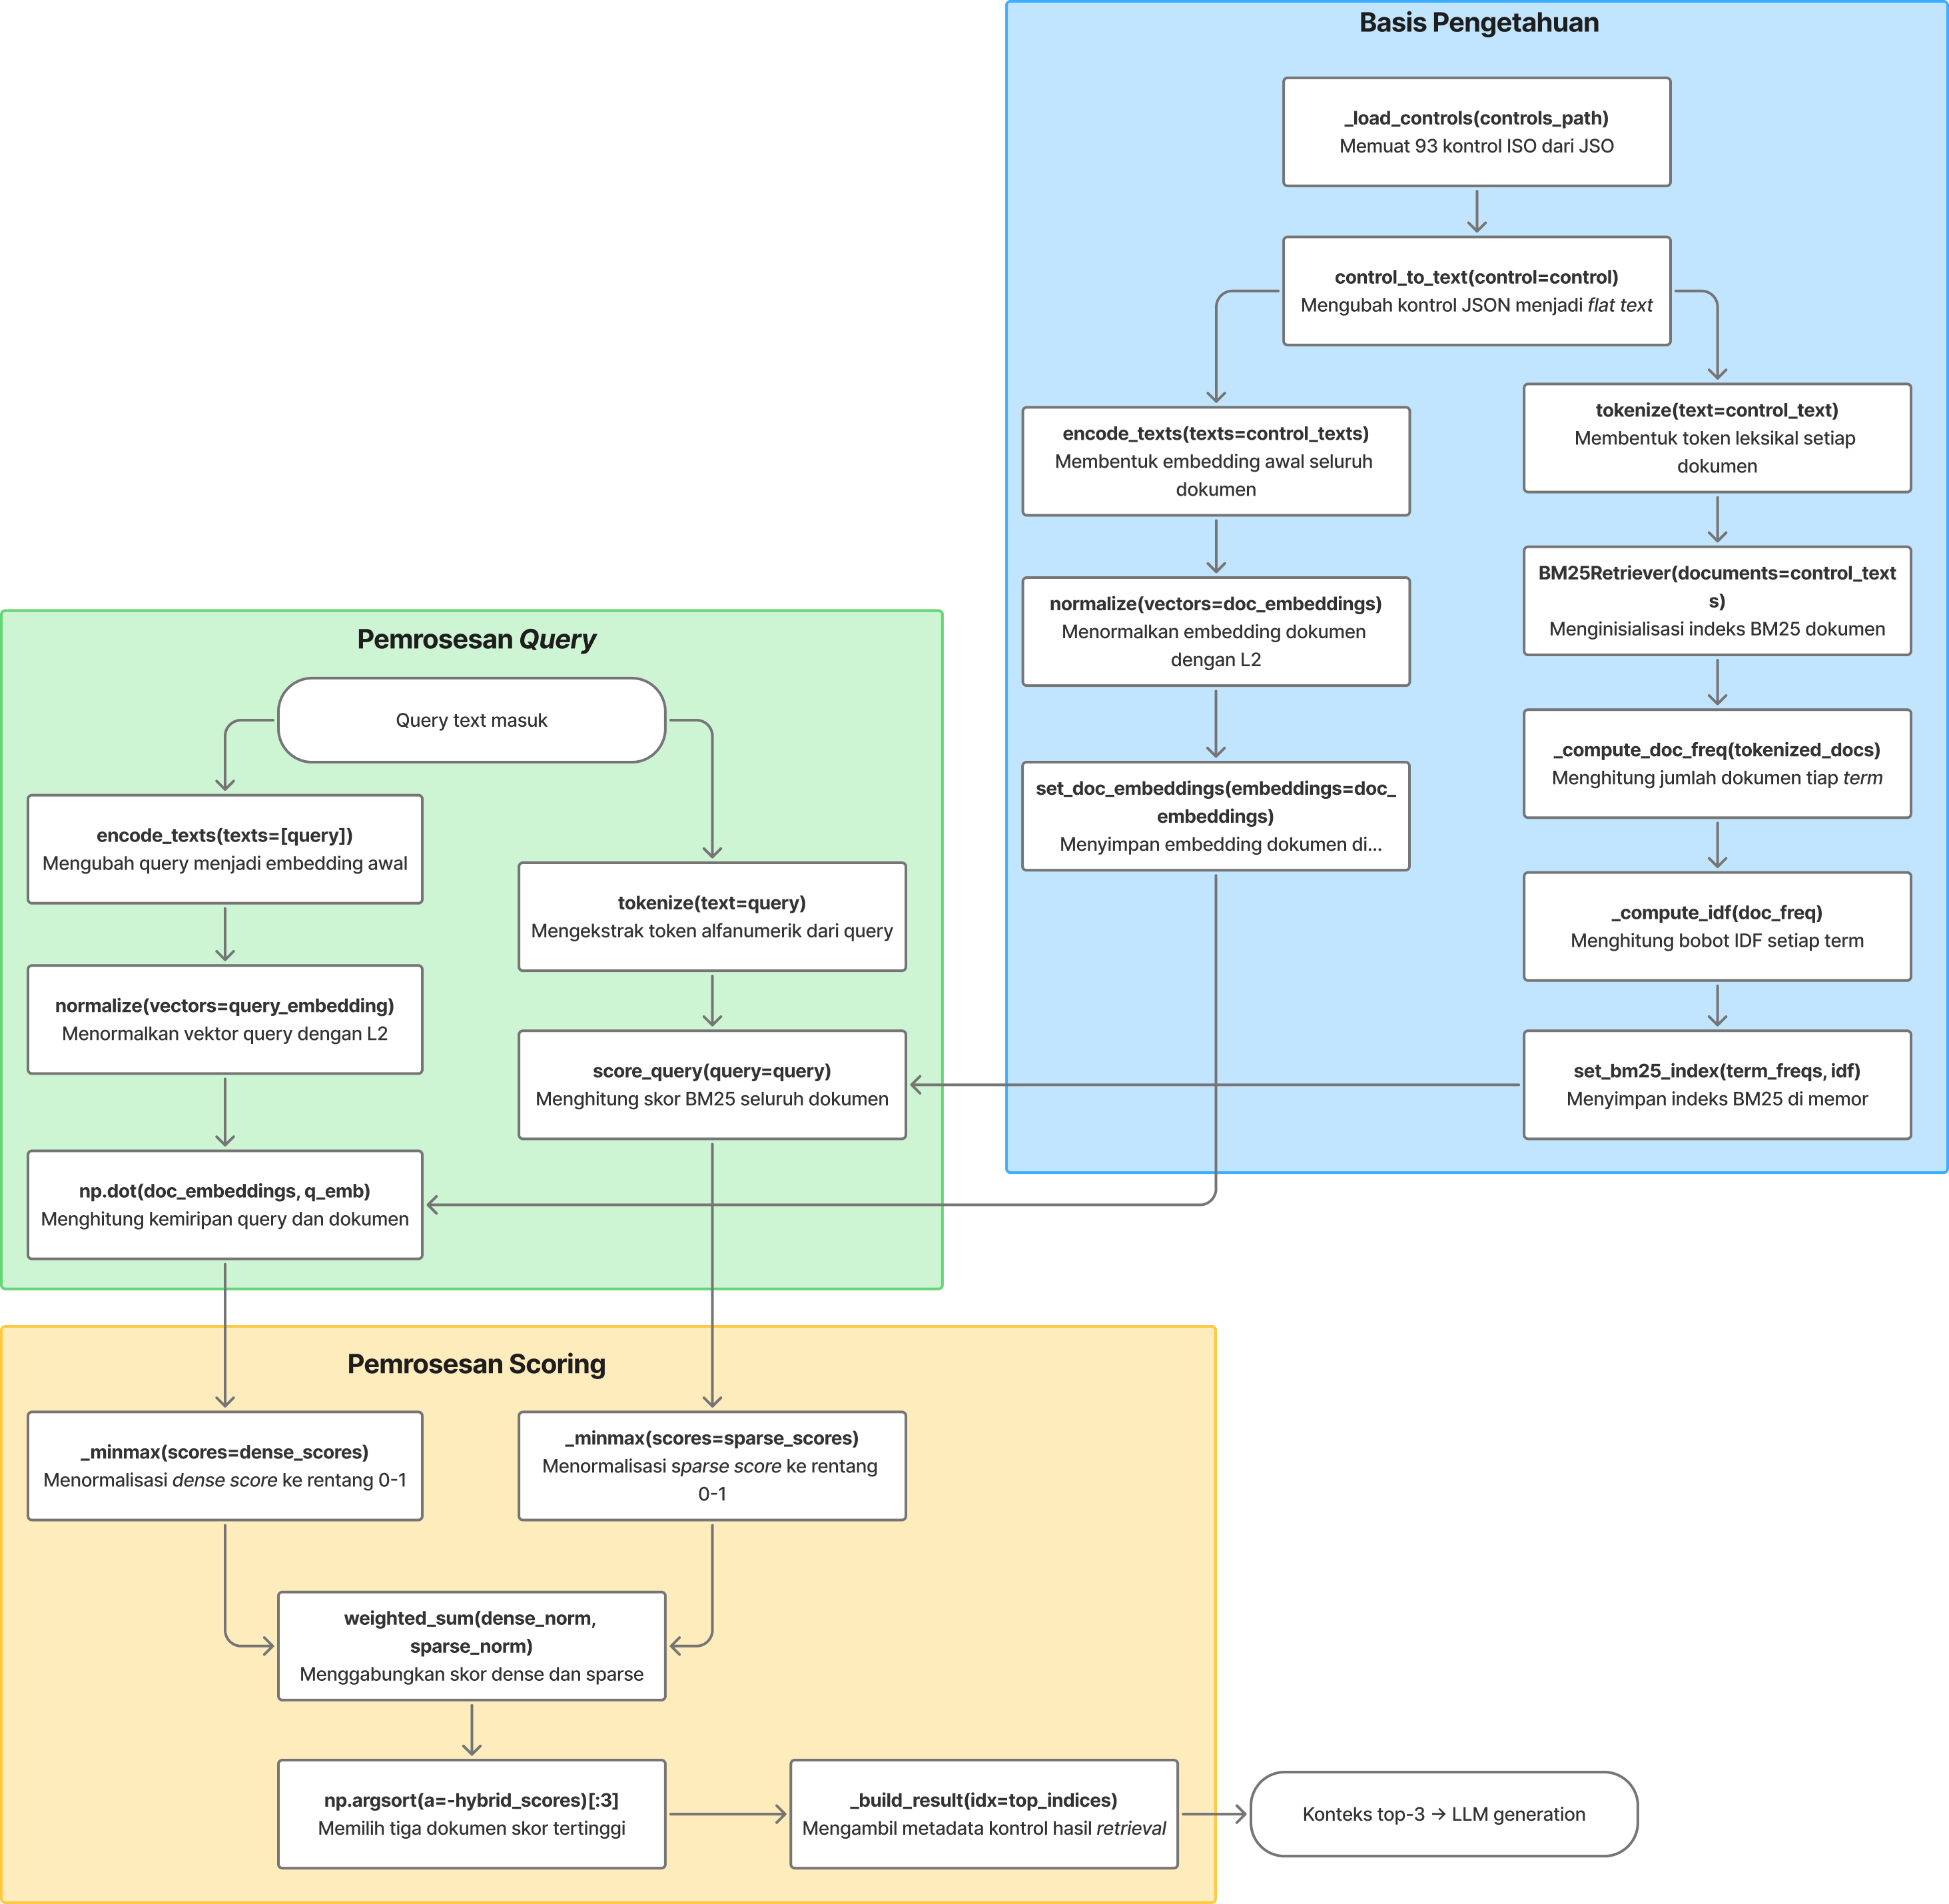
\includegraphics[width=\textwidth,keepaspectratio]{Gambar/3.6HybridComponentNew.png}
	\caption{Komponen hybrid retrieval pada sistem}
	\label{fig:retrieval_komponen}
\end{figure}

Berdasarkan alur yang ditunjukkan pada Gambar~\ref{fig:retrieval_komponen}, proses \textit{retrieval} dapat diuraikan ke dalam tiga tahap utama sebagai berikut.

\begin{enumerate}
\item \textbf{Basis Pengetahuan}

Tahap Basis Pengetahuan merupakan fase inisialisasi yang dijalankan saat sistem dimulai untuk menyiapkan seluruh representasi dokumen kontrol ISO. Pada tahap ini, data kontrol ISO dimuat dari berkas JSON, dikonversi menjadi representasi teks, kemudian diproses melalui jalur \textit{dense} untuk membentuk \textit{embedding} dokumen dan jalur \textit{sparse} untuk membangun indeks BM25. Hasil dari fase ini disimpan dalam memori agar dapat digunakan kembali ketika \textit{query} pengguna diproses.

\begin{enumerate}[label=\alph*., leftmargin=1.1cm]
\item \textbf{\texttt{\_load\_controls(controls\_path)}}: Proses ini memuat data basis pengetahuan dari berkas JSON yang berisi 93 kontrol ISO. Hasil pemuatan data menjadi daftar kontrol yang akan digunakan sebagai korpus dokumen pada proses \textit{retrieval}.

\item \textbf{\texttt{control\_to\_text(control=control)}}: Proses ini mengubah satu data kontrol ISO berbentuk JSON menjadi representasi teks datar (\textit{flat text}). Representasi teks ini menggabungkan atribut penting seperti judul, objektif, deskripsi, serta atribut pengayaan yang tersedia agar dokumen memiliki konteks yang lebih lengkap.

\item \textbf{\texttt{encode\_texts(texts=control\_texts)}}: Proses ini mengubah seluruh representasi teks kontrol ISO menjadi vektor \textit{embedding}. Vektor ini merepresentasikan makna semantik dokumen sehingga dapat dibandingkan dengan \textit{query} pada ruang vektor yang sama.

\item \textbf{\texttt{normalize(vectors=doc\_embeddings)}}: Proses ini melakukan normalisasi L2 pada vektor \textit{embedding} dokumen. Normalisasi dilakukan agar perhitungan \textit{dot product} antara \textit{query} dan dokumen setara dengan \textit{cosine similarity}.

\item \textbf{\texttt{HybridRetriever.doc\_embeddings}}: Proses ini menyimpan vektor \textit{embedding} dokumen pada atribut \texttt{doc\_embeddings}. Penyimpanan dilakukan secara \textit{in-memory} sehingga indeks vektor dapat digunakan langsung saat sistem menghitung \textit{dense score}.

\item \textbf{\texttt{tokenize(text=control\_text)}}: Proses ini mengubah representasi teks dokumen menjadi daftar token leksikal. Tokenisasi dilakukan dengan mengubah teks menjadi huruf kecil dan mengambil karakter alfanumerik agar dokumen siap diproses oleh BM25.

\item \textbf{\texttt{BM25Retriever(documents=control\_texts)}}: Proses ini menginisialisasi indeks BM25 berdasarkan seluruh teks kontrol ISO. Inisialisasi ini membentuk struktur data yang diperlukan untuk menghitung kecocokan kata kunci antara \textit{query} dan dokumen.

\item \textbf{\texttt{\_compute\_doc\_freq(tokenized\_docs)}}: Proses ini menghitung jumlah dokumen yang mengandung setiap \textit{term}. Nilai \textit{document frequency} digunakan sebagai dasar untuk menentukan seberapa umum atau spesifik suatu \textit{term} dalam korpus.

\item \textbf{\texttt{\_compute\_idf(doc\_freq)}}: Proses ini menghitung nilai \textit{inverse document frequency} untuk setiap \textit{term}. Nilai IDF memberi bobot lebih tinggi pada \textit{term} yang lebih jarang muncul sehingga dokumen dengan kata kunci spesifik dapat diberi skor lebih relevan.

\item \textbf{\texttt{BM25 index}}: Proses ini menyimpan informasi \textit{term frequency}, panjang dokumen, rata-rata panjang dokumen, dan IDF. Informasi tersebut digunakan kembali pada tahap Pemrosesan \textit{Query} untuk menghitung \textit{sparse score}.
\end{enumerate}

\item \textbf{Pemrosesan \textit{Query}}

Tahap Pemrosesan \textit{Query} dijalankan setiap kali pengguna memasukkan pertanyaan atau kebutuhan informasi. Pada tahap ini, \textit{query} diproses melalui dua jalur yang sama dengan dokumen, yaitu jalur \textit{dense} untuk menghasilkan skor kemiripan semantik dan jalur \textit{sparse} untuk menghasilkan skor kecocokan kata kunci. Hasil dari tahap ini berupa \textit{dense score} dan \textit{sparse score} untuk seluruh kontrol ISO.

\begin{enumerate}[label=\alph*., leftmargin=1.1cm]
\item \textbf{\texttt{encode\_texts(texts=[query])}}: Proses ini mengubah \textit{query} pengguna menjadi vektor \textit{embedding}. Karena fungsi yang sama digunakan pada dokumen dan \textit{query}, keduanya berada pada ruang representasi semantik yang sama.

\item \textbf{\texttt{normalize(vectors=query\_embedding)}}: Proses ini menormalkan vektor \textit{query} menggunakan normalisasi L2. Normalisasi membuat perhitungan kemiripan antara \textit{query} dan dokumen dapat dilakukan secara konsisten menggunakan \textit{dot product}.

\item \textbf{\texttt{np.dot(doc\_embeddings, q\_emb)}}: Proses ini menghitung hasil \textit{dot product} antara vektor \textit{query} dan seluruh \textit{embedding} dokumen. Hasilnya adalah \textit{dense score} yang merepresentasikan tingkat kemiripan semantik \textit{query} terhadap 93 kontrol ISO.

\item \textbf{\texttt{tokenize(text=query)}}: Proses ini mengubah \textit{query} menjadi daftar token leksikal. Tokenisasi \textit{query} menggunakan aturan yang sama dengan dokumen agar pencocokan kata kunci pada BM25 berjalan konsisten.

\item \textbf{\texttt{score\_query(query=query)}}: Proses ini menghitung skor BM25 antara \textit{query} dan seluruh dokumen. Skor dihitung berdasarkan kombinasi \textit{term frequency}, IDF, dan normalisasi panjang dokumen sehingga menghasilkan \textit{sparse score} untuk 93 kontrol ISO.
\end{enumerate}

\item \textbf{Pemrosesan \textit{Scoring}}

Tahap Pemrosesan \textit{Scoring} berfungsi untuk menggabungkan \textit{dense score} dan \textit{sparse score} menjadi satu skor akhir. Kedua jenis skor terlebih dahulu dinormalisasi karena memiliki skala yang berbeda. Setelah itu, skor digabungkan menggunakan \textit{weighted sum}, diurutkan, dan digunakan untuk memilih dokumen teratas sebagai hasil \textit{retrieval}.

\begin{enumerate}[label=\alph*., leftmargin=1.1cm]
\item \textbf{\texttt{\_minmax(scores=dense\_scores)}}: Proses ini menormalisasi \textit{dense score} ke rentang 0 sampai 1. Normalisasi ini diperlukan agar skor semantik memiliki skala yang sebanding dengan skor BM25.

\item \textbf{\texttt{\_minmax(scores=sparse\_scores)}}: Proses ini menormalisasi \textit{sparse score} ke rentang 0 sampai 1. Normalisasi dilakukan secara terpisah dari \textit{dense score} karena kedua skor berasal dari metode yang berbeda.

\item \textbf{\texttt{weighted\_sum(dense\_norm, sparse\_norm)}}: Proses ini menggabungkan skor \textit{dense} dan \textit{sparse} yang telah dinormalisasi. Formula yang digunakan adalah $\textit{hybrid\_score} = w_{\textit{dense}} \times \textit{dense\_norm} + w_{\textit{sparse}} \times \textit{sparse\_norm}$.

\item \textbf{\texttt{np.argsort(a=-hybrid\_scores)[:3]}}: Proses ini mengurutkan dokumen berdasarkan \textit{hybrid score} secara menurun. Tiga dokumen dengan skor tertinggi dipilih sebagai kandidat paling relevan.

\item \textbf{\texttt{\_build\_result(idx=top\_indices)}}: Proses ini mengambil metadata dokumen terpilih seperti \texttt{control\_id}, \texttt{title}, \texttt{objective}, dan \texttt{description}. Metadata beserta skor \textit{dense}, \textit{sparse}, dan \textit{hybrid} digunakan sebagai hasil akhir tahap \textit{retrieval}.
\end{enumerate}

\end{enumerate}


\subsubsection{Perancangan Komponen \textit{Rerank} pada Sistem}

Komponen \textit{reranking} pada penelitian ini menggunakan model \textit{cross-encoder} yang dipilih berdasarkan analisis perbandingan pada Subbab~2.3.4.

\vspace{1.5em}
\noindent\textbf{Pemilihan Model \textit{Reranker}}

Berdasarkan analisis perbandingan model \textit{reranker} pada Subbab~2.3.4, BAAI/bge-reranker-v2-m3 dipilih sebagai model \textit{reranker}. Model ini dipilih karena menggabungkan bukti empiris pada domain regulasi yang menunjukkan peningkatan signifikan pada kualitas peringkat, dukungan multilingual untuk lebih dari 100 bahasa yang esensial untuk \textit{query} berbahasa Indonesia, serta kemudahan implementasi sebagai model \textit{cross-encoder} yang bersifat \textit{plug-and-play}.

Perancangan komponen \textit{rerank} pada sistem dilakukan untuk meningkatkan kualitas urutan dokumen yang telah diperoleh dari tahap \textit{hybrid retrieval}. Pada rancangan ini, sistem tidak langsung menggunakan hasil \textit{hybrid retrieval} sebagai keluaran akhir, tetapi terlebih dahulu membentuk \textit{candidate pool} dan mengevaluasi ulang kandidat tersebut menggunakan model \textit{cross-encoder}. Dengan demikian, hasil akhir tidak hanya mempertimbangkan skor gabungan \textit{dense} dan \textit{sparse}, tetapi juga mempertimbangkan interaksi langsung antara \textit{query} dan dokumen kandidat.

\begin{figure}[H]
	\centering
	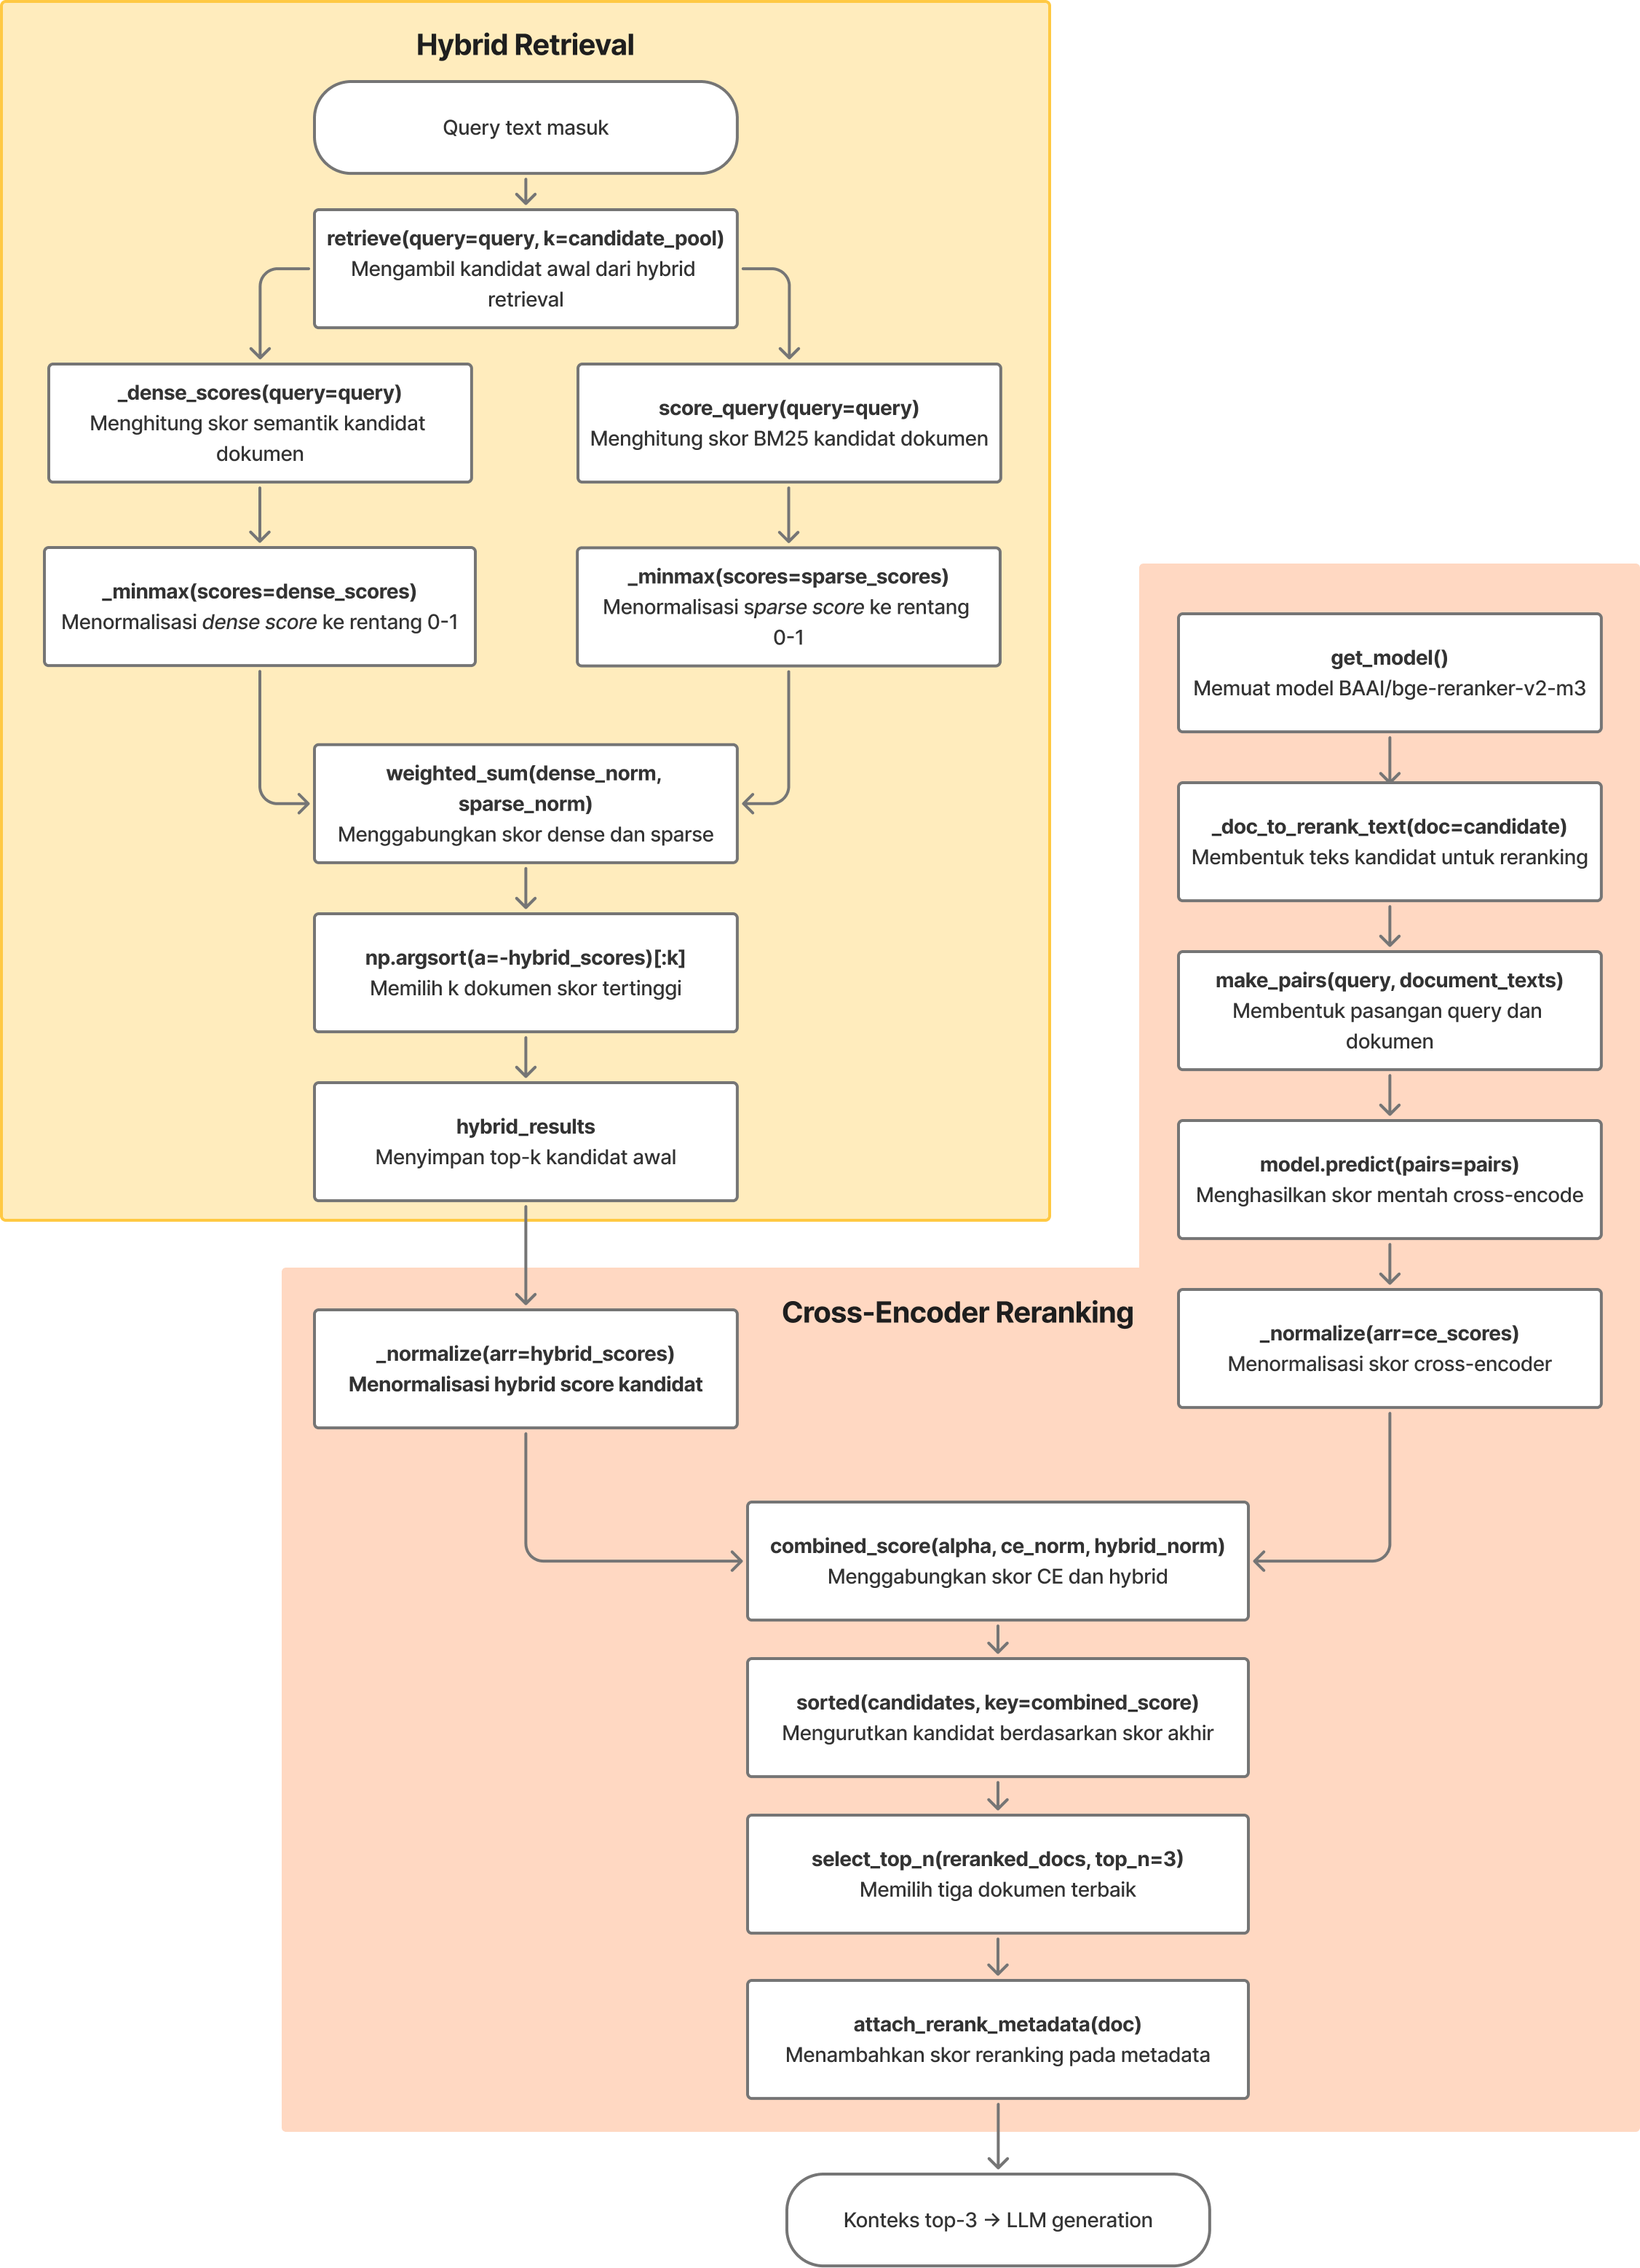
\includegraphics[width=\textwidth]{Gambar/3.7RerankerComponentNew.png}
	\caption{Komponen cross-encoder reranking pada sistem}
	\label{fig:reranking_komponen}
\end{figure}

\newpage

Berdasarkan alur yang ditunjukkan pada Gambar~\ref{fig:reranking_komponen}, proses \textit{rerank} dapat diuraikan ke dalam dua tahap utama, yaitu tahap \textit{hybrid retrieval} dan tahap \textit{cross-encoder reranking}.

\begin{enumerate}
\item \textbf{Tahap \textit{Hybrid Retrieval}}

Tahap \textit{hybrid retrieval} berfungsi sebagai tahap awal untuk menghasilkan kandidat dokumen yang akan dievaluasi ulang oleh \textit{reranker}. Pada tahap ini, sistem memproses \textit{query} menggunakan mekanisme \textit{dense retrieval} dan \textit{sparse retrieval}, menormalisasi skor dari kedua jalur, menggabungkannya menjadi \textit{hybrid score}, lalu memilih sejumlah kandidat teratas sebagai \textit{candidate pool}. Dalam rancangan ini, \textit{candidate pool} digunakan sebagai masukan untuk tahap \textit{cross-encoder reranking}.

\begin{enumerate}[label=\alph*., leftmargin=1.1cm]
\item \textbf{\texttt{retrieve(query=query, k=candidate\_pool)}}: Proses ini mengambil kandidat awal menggunakan komponen \textit{hybrid retrieval}. Parameter \texttt{k} menentukan jumlah kandidat yang masuk ke \textit{candidate pool} sebelum dilakukan \textit{reranking}.

\item \textbf{\texttt{\_dense\_scores(query=query)}}: Proses ini menghitung skor semantik antara \textit{query} dan seluruh dokumen menggunakan operasi \textit{dot product}. Skor yang dihasilkan merepresentasikan kemiripan makna antara kebutuhan informasi pengguna dan dokumen kontrol ISO.

\item \textbf{\texttt{score\_query(query=query)}}: Proses ini menghitung skor BM25 antara \textit{query} dan seluruh dokumen. Skor ini merepresentasikan kecocokan kata kunci berdasarkan \textit{term frequency}, IDF, dan normalisasi panjang dokumen.

\item \textbf{\texttt{\_minmax(scores=dense\_scores)}}: Proses ini menormalisasi \textit{dense score} ke rentang 0 sampai 1. Normalisasi diperlukan agar skor semantik memiliki skala yang sebanding dengan skor dari jalur \textit{sparse}.

\item \textbf{\texttt{\_minmax(scores=sparse\_scores)}}: Proses ini menormalisasi \textit{sparse score} ke rentang 0 sampai 1. Normalisasi dilakukan secara terpisah karena skor BM25 memiliki skala berbeda dari skor \textit{dense}.

\item \textbf{\texttt{weighted\_sum(dense\_norm, sparse\_norm)}}: Proses ini menggabungkan skor \textit{dense} dan \textit{sparse} yang telah dinormalisasi. Hasil penggabungan membentuk \textit{hybrid score} yang digunakan untuk menentukan kandidat awal.

\item \textbf{\texttt{np.argsort(a=-hybrid\_scores)[:k]}}: Proses ini mengurutkan dokumen berdasarkan \textit{hybrid score} secara menurun dan memilih kandidat dengan skor tertinggi. Kandidat terpilih menjadi \textit{candidate pool} untuk tahap \textit{reranking}.

\item \textbf{\texttt{hybrid\_results}}: Proses ini menyimpan daftar kandidat awal hasil \textit{hybrid retrieval}. Setiap kandidat mempertahankan metadata dokumen dan skor \textit{dense}, \textit{sparse}, serta \textit{hybrid} untuk digunakan pada tahap berikutnya.
\end{enumerate}

\item \textbf{\textit{Cross-Encoder Reranking}}

Tahap \textit{cross-encoder reranking} berfungsi untuk mengevaluasi ulang kandidat dokumen dari tahap \textit{hybrid retrieval}. Pada tahap ini, setiap kandidat diubah menjadi teks representatif, kemudian dipasangkan dengan \textit{query} dan diproses oleh model \textit{cross-encoder}. Skor \textit{cross-encoder} dinormalisasi dan dikombinasikan dengan skor \textit{hybrid} untuk menghasilkan \textit{combined score}. Skor akhir ini digunakan untuk menentukan urutan dokumen terbaik.

\begin{enumerate}[label=\alph*., leftmargin=1.1cm]
\item \textbf{\texttt{get\_model()}}: Proses ini memuat model \textit{BAAI/bge-reranker-v2-m3} dengan mekanisme \textit{lazy loading}. Model digunakan untuk menghitung relevansi pasangan \textit{query} dan dokumen secara langsung.

\item \textbf{\texttt{\_doc\_to\_rerank\_text(doc=candidate)}}: Proses ini membentuk teks kandidat yang digunakan pada tahap \textit{reranking}. Teks kandidat memuat atribut dokumen seperti judul, objektif, deskripsi, kata kunci, dan indikator audit agar konteks dokumen lebih lengkap.

\item \textbf{\texttt{make\_pairs(query, document\_texts)}}: Proses ini membentuk pasangan antara \textit{query} dan teks dokumen kandidat. Pasangan ini menjadi masukan utama bagi model \textit{cross-encoder} untuk melakukan penilaian relevansi.

\item \textbf{\texttt{model.predict(pairs=pairs)}}: Proses ini menghasilkan skor mentah \textit{cross-encoder} untuk setiap pasangan \textit{query} dan dokumen. Skor tersebut menunjukkan tingkat relevansi kandidat berdasarkan interaksi langsung antara dua teks.

\item \textbf{\texttt{\_normalize(arr=ce\_scores)}}: Proses ini menormalisasi skor \textit{cross-encoder} ke rentang 0 sampai 1. Normalisasi diperlukan agar skor \textit{cross-encoder} dapat digabungkan dengan skor \textit{hybrid}.

\item \textbf{\texttt{\_normalize(arr=hybrid\_scores)}}: Proses ini menormalisasi \textit{hybrid score} kandidat ke rentang 0 sampai 1. Skor ini digunakan sebagai sinyal relevansi awal dari tahap \textit{retrieval}.

\item \textbf{\texttt{combined\_score(alpha, ce\_norm, hybrid\_norm)}}: Proses ini menggabungkan skor \textit{cross-encoder} dan skor \textit{hybrid} yang telah dinormalisasi. Formula yang digunakan adalah $\textit{combined\_score} = \alpha \times \textit{ce\_norm} + (1 - \alpha) \times \textit{hybrid\_norm}$.

\item \textbf{\texttt{sorted(candidates, key=combined\_score)}}: Proses ini mengurutkan seluruh kandidat berdasarkan \textit{combined score} secara menurun. Kandidat dengan skor akhir tertinggi ditempatkan pada peringkat teratas.

\item \textbf{\texttt{select\_top\_n(reranked\_docs, top\_n=3)}}: Proses ini memilih tiga dokumen terbaik setelah proses \textit{reranking}. Dokumen terpilih menjadi hasil akhir yang digunakan sebagai konteks pada tahap generasi.

\item \textbf{\texttt{attach\_rerank\_metadata(doc)}}: Proses ini menambahkan informasi hasil \textit{reranking} ke metadata dokumen. Informasi tersebut mencakup \texttt{rerank\_score}, \texttt{rerank\_score\_norm}, \texttt{hybrid\_score\_norm}, dan \texttt{combined\_score} untuk mendukung transparansi hasil.
\end{enumerate}
\end{enumerate}

\section{Alur Tugas Akhir}

Penelitian ini dilaksanakan melalui serangkaian tahapan yang dirancang secara sistematis untuk menjawab hipotesis dan tujuan penelitian secara komprehensif. Setiap tahapan memiliki luaran yang saling berkaitan dan digunakan sebagai dasar pada tahapan berikutnya, sehingga keseluruhan proses penelitian dapat berjalan secara terstruktur dan berkesinambungan. Alur penelitian dimulai dari proses studi literatur dan identifikasi permasalahan, dilanjutkan dengan persiapan data dan kebutuhan penelitian, perancangan sistem dan metode yang digunakan, pelaksanaan pengujian dan eksperimen, hingga tahap analisis hasil evaluasi dan penyusunan kesimpulan akhir penelitian.

Gambar~\ref{fig:alur_penelitian} menunjukkan diagram alur penelitian secara keseluruhan yang menggambarkan hubungan antar tahapan penelitian mulai dari tahap persiapan hingga proses evaluasi akhir.

\begin{figure}[H]
	\centering
	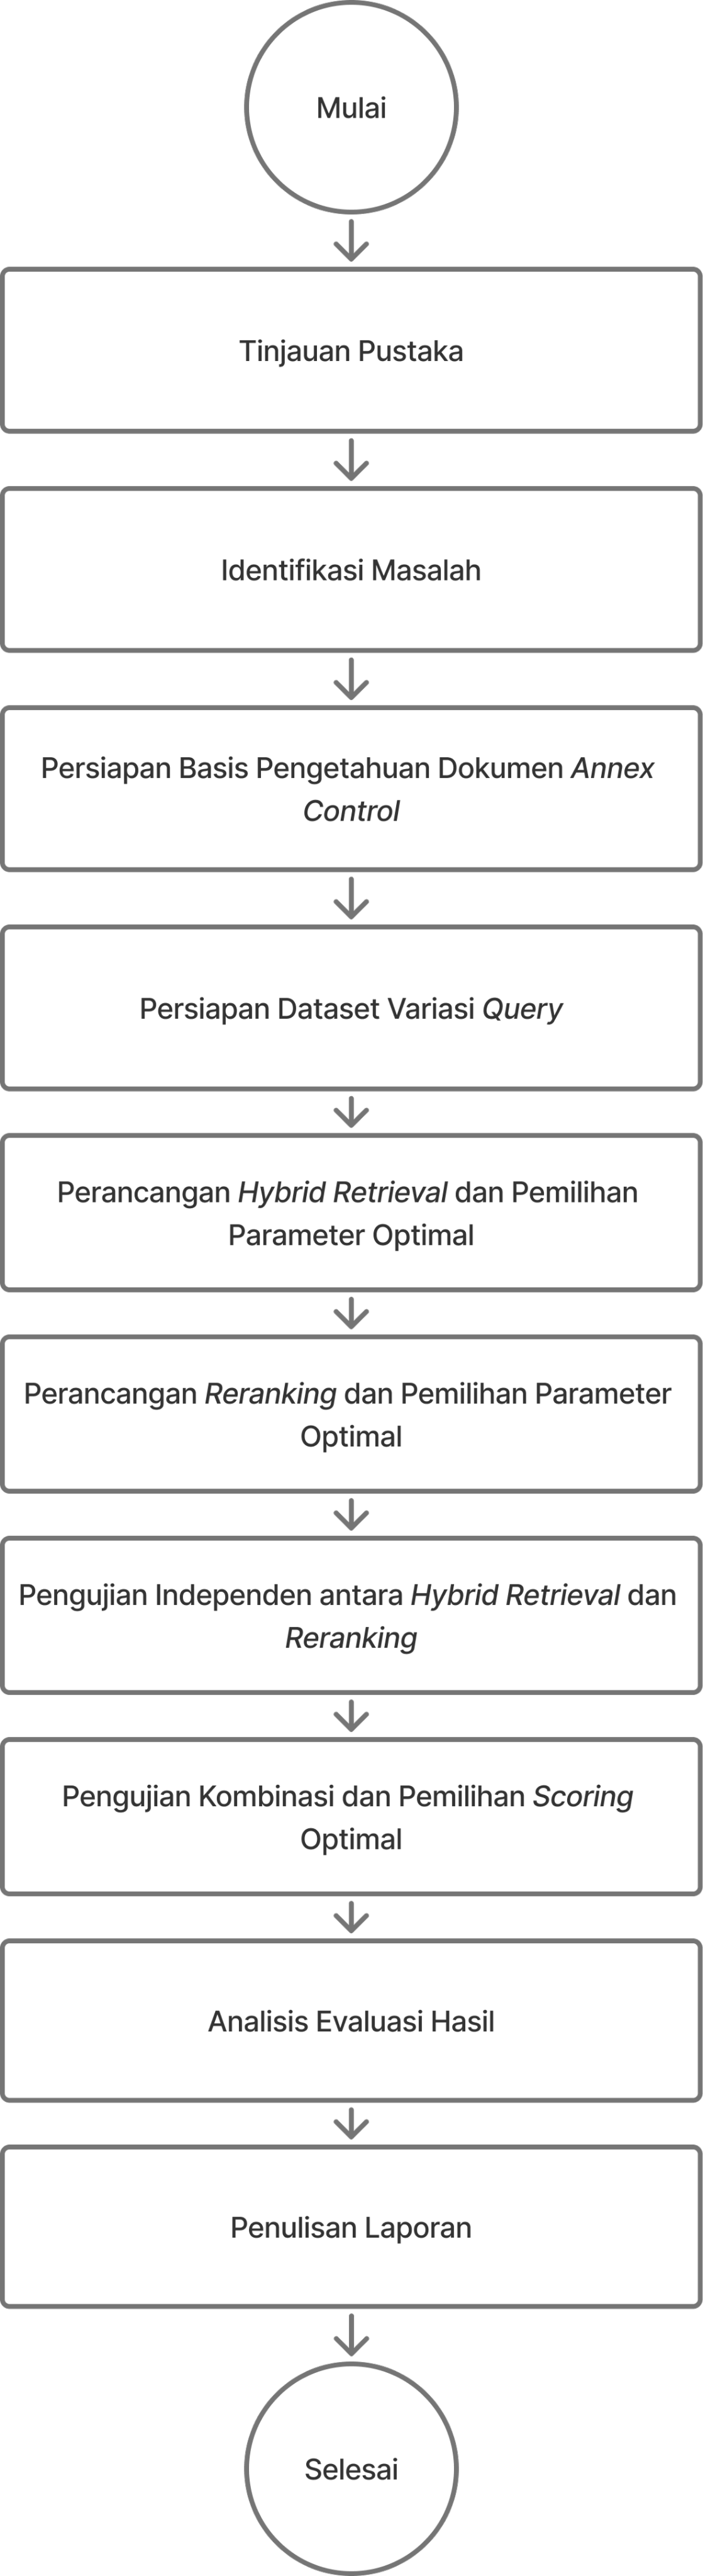
\includegraphics[width=0.7125\textwidth,height=0.585\textheight,keepaspectratio]{Gambar/3.8AlurPenelitian.png}
	\caption{Alur penelitian}
	\label{fig:alur_penelitian}
\end{figure}

\subsection{Tinjauan Pustaka}

Langkah pertama pada penelitian ini adalah melakukan tinjauan pustaka untuk memperoleh pemahaman terkait perkembangan penelitian yang relevan dengan topik penelitian. Proses tinjauan pustaka dilakukan dengan menelusuri berbagai publikasi ilmiah, khususnya pada IEEE dan sumber ilmiah bereputasi lainnya. Beberapa kata kunci yang digunakan dalam pencarian literatur antara lain ``\textit{RAG for Auditing}'', ``\textit{Retrieval Strategy Optimization}'', ``\textit{Information Retrieval}'', dan ``\textit{Cross-Encoder Reranking}''. Kata kunci tersebut dipilih karena memiliki keterkaitan langsung dengan fokus penelitian, yaitu evaluasi strategi \textit{retrieval} dan \textit{reranking} pada \textit{pipeline} RAG.

Seperti yang telah dijelaskan pada Subbab 2.1, terdapat beberapa tema utama yang ditemukan pada penelitian-penelitian terdahulu. Variasi penelitian yang ditemukan meliputi domain penerapan sistem RAG, jenis pendekatan \textit{hybrid retrieval} yang digunakan, pemanfaatan metode \textit{cross-encoder reranking}, serta strategi pembobotan \textit{score fusion} dan penyesuaian parameter untuk memperoleh performa \textit{retrieval} yang optimal. Berdasarkan hasil tinjauan pustaka tersebut, penelitian ini dirancang dengan fokus pada evaluasi performa kombinasi \textit{hybrid retrieval} dan \textit{cross-encoder reranking} dalam meningkatkan kualitas hasil \textit{retrieval} pada dokumen ISO/IEC 27001:2022.

\subsection{Identifikasi Masalah}

Berdasarkan hasil tinjauan pustaka, telah ditemukan berbagai penelitian yang menerapkan pendekatan \textit{Retrieval-Augmented Generation} (RAG) khususnya \textit{Information Retrieval} pada domain tertentu, seperti regulasi perpajakan, dokumen keuangan, maupun kebijakan privasi. Penelitian-penelitian tersebut menunjukkan bahwa kombinasi \textit{hybrid retrieval} dan \textit{reranking} mampu meningkatkan relevansi hasil pencarian pada dokumen yang bersifat regulatif dan berbasis teks.

Namun, hingga saat penelitian ini dilakukan, masih ditemukan keterbatasan penelitian yang secara khusus membahas penerapan strategi \textit{retrieval} pada standar ISO/IEC 27001:2022, terutama pada Annex A domain A.5 hingga A.8. Karakteristik dokumen ISO 27001 memiliki tantangan tersendiri karena beberapa \textit{annex control} memiliki konteks, istilah, dan tujuan kontrol yang saling berdekatan, sehingga suatu kondisi audit dapat berkaitan dengan lebih dari satu kontrol keamanan. Hal tersebut menyebabkan proses klasifikasi dan pemetaan kontrol menjadi lebih rentan kesalahan dibandingkan domain regulasi umum lainnya.

Selain itu, pada \textit{pipeline Retrieval-Augmented Generation} (RAG), kualitas hasil \textit{retrieval} memiliki pengaruh langsung terhadap ketepatan proses \textit{generation}. Apabila dokumen atau kontrol yang dipilih pada tahap \textit{retrieval} tidak relevan, maka hasil \textit{generation} yang digunakan untuk proses pemetaan terhadap \textit{Statement of Applicability} (SoA) berpotensi menjadi kurang akurat. Oleh karena itu, penelitian ini difokuskan pada evaluasi komparatif strategi \textit{retrieval}, khususnya \textit{hybrid retrieval}, \textit{cross-encoder reranking}, serta kombinasi keduanya, untuk mengidentifikasi pendekatan yang mampu memberikan performa \textit{retrieval} paling optimal pada dokumen ISO/IEC 27001:2022. Penelitian ini tidak bertujuan untuk mengembangkan \textit{pipeline} RAG secara \textit{end-to-end}, melainkan menghasilkan rekomendasi strategi \textit{information retrieval} yang efektif untuk mendukung proses pemetaan kontrol keamanan dan implementasi sistem audit keamanan informasi berbasis ISO 27001 di masa mendatang.

\subsection{Persiapan Basis Pengetahuan Dokumen Kontrol \textit{Annex}}

Tahap persiapan basis pengetahuan dilakukan dengan mengumpulkan informasi terkait \textit{annex control} berdasarkan standar ISO/IEC 27001:2022, khususnya pada domain Annex A.5 hingga A.8. Sumber utama yang digunakan berasal dari dokumen resmi ``INTERNATIONAL STANDARD ISO/IEC 27001 Third Edition 2022-10''. Selain itu, informasi tambahan juga dikumpulkan dari berbagai sumber di internet seperti artikel implementasi keamanan informasi, dokumentasi audit, serta referensi praktik keamanan siber untuk memperkaya konteks tiap kontrol keamanan. Penambahan informasi tersebut dilakukan agar basis pengetahuan tidak hanya memuat definisi kontrol secara formal, tetapi juga mencakup istilah, konteks audit, dan variasi implementasi yang umum digunakan pada lingkungan nyata.

Seluruh informasi yang telah dikumpulkan kemudian direpresentasikan dalam format JSON (\textit{JavaScript Object Notation}), di mana setiap \textit{annex control} disimpan sebagai satu entitas data terstruktur. Struktur JSON mencakup atribut seperti identitas kontrol, deskripsi, panduan implementasi, kata kunci, indikator audit, aset terkait, dan prinsip keamanan dalam Bahasa Indonesia maupun Bahasa Inggris. Proses penyusunan dan pengisian atribut dilakukan secara manual oleh penulis untuk menjaga kesesuaian konteks dengan standar ISO 27001, serta dibantu dengan pemanfaatan \textit{Generative AI} untuk menghasilkan variasi istilah, pengayaan kata kunci, dan penyusunan atribut pendukung yang lebih lengkap.

\subsection{Persiapan \textit{Dataset} Variasi \textit{Query}}

Tahap persiapan \textit{dataset query} dilakukan dengan menyusun \textit{query} yang dibentuk dari dokumen asli milik Direktorat Teknologi Informasi Universitas Gadjah Mada (DTI UGM). Proses penyusunan \textit{query} dilakukan melalui pembacaan dan penelaahan manual terhadap dokumen kebijakan, prosedur, standar operasional, tata kelola, serta regulasi internal yang berkaitan dengan keamanan informasi dan pengelolaan teknologi informasi. Dari hasil pembacaan tersebut, kemudian diidentifikasi potongan informasi, kebutuhan audit, maupun pernyataan kebijakan yang berpotensi merepresentasikan kebutuhan pencarian informasi pada proses audit ISO/IEC 27001:2022. Berdasarkan konteks tersebut, \textit{query} kemudian dirumuskan secara manual dengan mempertahankan istilah, struktur bahasa, dan gaya penyampaian yang mendekati kondisi nyata pada lingkungan organisasi DTI UGM.

Setelah \textit{query} berhasil dibentuk, dilakukan proses penelaahan untuk menentukan \textit{ground truth annex control} yang sesuai terhadap masing-masing \textit{query}. Penentuan \textit{ground truth} dilakukan dengan mencocokkan konteks \textit{query} terhadap kontrol ISO/IEC 27001:2022 Annex A.5 hingga A.8 berdasarkan relevansi isi, tujuan pengendalian, serta cakupan keamanan informasi yang dibahas dalam dokumen sumber. Setiap \textit{query} dapat memiliki keterkaitan dengan satu atau lebih kontrol \textit{annex} sesuai kompleksitas konteks yang ditemukan.

\subsection{Perancangan \textit{Hybrid Retrieval} dan Pemilihan Parameter Optimal}

Perancangan metode \textit{hybrid retrieval} pada penelitian ini dilakukan dengan mengacu pada beberapa penelitian terdahulu, khususnya penelitian oleh Rustamov et al. dan Liu et al. yang menerapkan kombinasi \textit{sparse retrieval} menggunakan BM25 dan \textit{dense retrieval} berbasis model MiniLM. Pada penelitian ini, BM25 digunakan untuk menangkap kesesuaian istilah secara eksplisit, sedangkan \textit{dense retrieval} menggunakan model paraphrase-multilingual-MiniLM-L12-v2 untuk memahami keterkaitan makna semantik antara \textit{query} dan dokumen \textit{annex control}. Penggunaan model ini merupakan pengembangan dari penelitian sebelumnya yang banyak menggunakan model all-MiniLM-L6-v2 sebagai \textit{baseline dense retrieval}.

Pada penelitian ini dipilih model \textit{multilingual} karena kumpulan \textit{query} dan dokumen berasal dari lingkungan institusi pendidikan di Indonesia yang didominasi penggunaan Bahasa Indonesia serta istilah teknis berbahasa Inggris secara bersamaan. Selain itu, arsitektur L12 dengan 12 \textit{layer} dipilih karena memiliki kapasitas representasi semantik yang lebih baik dibandingkan varian L6, sehingga diharapkan lebih mampu menangkap hubungan makna pada \textit{query} audit yang bersifat implisit, panjang, dan kontekstual. Dengan demikian, model ini dinilai lebih sesuai untuk skenario \textit{retrieval} dokumen keamanan informasi pada domain DTI UGM yang memiliki karakteristik bahasa campuran dan konteks kebijakan yang kompleks.

Setelah metode \textit{hybrid retrieval} dirancang, tahap selanjutnya adalah melakukan pencarian parameter bobot \textit{score fusion} yang optimal melalui penyesuaian nilai $\alpha$ (\textit{alpha scoring}). Parameter $\alpha$ digunakan untuk mengatur proporsi kontribusi skor antara \textit{sparse retrieval} dan \textit{dense retrieval} pada proses penggabungan skor akhir. Pengujian dilakukan terhadap seluruh variasi \textit{query} yang digunakan dalam penelitian untuk menentukan kombinasi bobot yang mampu memberikan performa \textit{retrieval} terbaik sebelum integrasi metode \textit{reranking}. Hasil pencarian parameter ini kemudian digunakan sebagai konfigurasi dasar pada tahap eksperimen berikutnya agar proses \textit{score fusion} antara \textit{hybrid retrieval} dan \textit{cross-encoder reranking} dapat dilakukan secara konsisten dan terukur.

\subsection{Perancangan \textit{Reranking} dan Pemilihan Parameter Optimal}

Tahap perancangan \textit{reranking} dilakukan sebagai pengembangan dari rancangan \textit{hybrid retrieval} yang telah dibangun pada tahap sebelumnya. Pada proses ini, hasil \textit{retrieval} awal dari metode \textit{hybrid retrieval} digunakan sebagai \textit{candidate pool} yang akan diproses kembali untuk meningkatkan kualitas peringkat dokumen. Dengan pendekatan ini, sistem tidak melakukan proses \textit{reranking} terhadap seluruh dokumen pada korpus, melainkan hanya pada sejumlah dokumen dengan skor \textit{retrieval} tertinggi hasil dari proses \textit{hybrid retrieval}. Pendekatan tersebut dipilih untuk menjaga efisiensi komputasi sekaligus mempertahankan kualitas relevansi hasil pencarian.

Metode \textit{reranking} yang digunakan pada penelitian ini adalah pendekatan \textit{cross-encoder} menggunakan model BAAI/bge-reranker-v2-m3 yang mendukung pemrosesan multibahasa, termasuk Bahasa Indonesia. Pemilihan model BGE \textit{reranker} juga didasarkan pada beberapa penelitian sebelumnya oleh Rustamov et al. menggunakan seri model BGE sebagai pendekatan \textit{retrieval} dan \textit{reranking} karena memiliki performa \textit{semantic matching} yang baik pada tugas \textit{information retrieval} modern. Selain itu, penelitian oleh Elkiran-Rasheed menunjukkan bahwa model BAAI/bge-reranker-base mampu menghasilkan nilai akurasi terbaik dibandingkan beberapa model \textit{reranker} lainnya pada proses evaluasi \textit{retrieval}.

Berdasarkan pertimbangan tersebut, penelitian ini menggunakan varian BAAI/bge-reranker-v2-m3 karena memiliki kemampuan \textit{multilingual} dan kapasitas pemahaman konteks yang lebih sesuai dengan karakteristik dokumen kebijakan serta \textit{query} audit pada lingkungan institusi pendidikan di Indonesia. Setelah rancangan \textit{reranking} dibangun, dilakukan pengujian terhadap beberapa variasi jumlah \textit{candidate pool} yang diambil dari hasil \textit{hybrid retrieval} untuk menentukan nilai top-$n$ yang paling optimal untuk proses \textit{reranking} dilakukan. Pengujian ini bertujuan memperoleh keseimbangan antara kualitas relevansi dan efisiensi komputasi, sehingga proses \textit{score fusion} antara \textit{hybrid retrieval} dan \textit{cross-encoder reranking} dapat menghasilkan performa \textit{retrieval} yang optimal.

\subsection{Pengujian Kombinasi dan Pemilihan \textit{Scoring} Optimal}

Setelah perancangan metode \textit{hybrid retrieval} dan \textit{cross-encoder reranking} selesai dilakukan, tahap selanjutnya adalah melakukan pengujian kombinasi kedua metode melalui mekanisme pembobotan \textit{score fusion}. Pada tahap ini, pengujian dilakukan secara komprehensif dengan memvariasikan parameter $\alpha$ (\textit{alpha scoring}) untuk menentukan proporsi skor yang paling optimal antara hasil \textit{hybrid retrieval} dan skor dari \textit{reranking}, dengan urutan pembobotan \textit{hybrid}:\textit{cross-encoder}. Dalam kerangka ini, pengujian \textit{hybrid retrieval} secara independen direpresentasikan oleh parameter pembobotan 1:0, pengujian \textit{reranker} secara independen direpresentasikan oleh parameter pembobotan 0:1, sedangkan konfigurasi dengan pembobotan lainnya merepresentasikan kombinasi kedua metode.

Pada tahap ini, \textit{hybrid retrieval} menggunakan parameter bobot $\alpha$ paling optimal antara komponen \textit{dense retrieval} dan \textit{sparse retrieval} yang diperoleh dari tahap sebelumnya, sedangkan \textit{reranking} menggunakan jumlah \textit{candidate pool} terbaik. Proses eksperimen dilakukan pada seluruh \textit{query} yang dibentuk dari dokumen kebijakan Direktorat Teknologi Informasi (DTI) UGM. Setiap kombinasi parameter dievaluasi menggunakan metrik \textit{Information Retrieval} seperti Hit@3, Recall@3, MAP@3, dan NDCG@3 untuk mengidentifikasi konfigurasi bobot \textit{score fusion} yang memberikan performa paling optimal. Pengujian ini bertujuan untuk mengevaluasi kualitas performa masing-masing pendekatan baik secara independen maupun dalam bentuk kombinasi, sehingga dapat diketahui kontribusi dan karakteristik tiap metode terhadap hasil \textit{retrieval} sekaligus ditentukan pendekatan kombinasi yang paling efektif dalam meningkatkan relevansi hasil pencarian pada proses pemetaan \textit{annex control} ISO/IEC 27001:2022.

\subsection{Analisis Evaluasi Hasil}

Tahap analisis evaluasi hasil dilakukan setelah seluruh proses pengujian terhadap metode \textit{hybrid retrieval}, \textit{cross-encoder reranking}, dan kombinasi bobot \textit{score fusion} selesai dilaksanakan. Pada tahap ini, hasil evaluasi dibandingkan untuk menganalisis performa masing-masing pendekatan, baik secara independen maupun dalam bentuk kombinasi. Analisis dilakukan menggunakan beberapa metrik \textit{Information Retrieval} seperti Hit@3, Recall@3, MAP@3, dan NDCG@3 untuk melihat tingkat relevansi dan kualitas peringkat dokumen yang dihasilkan oleh setiap metode. Selain itu, tahap ini juga digunakan untuk mengamati pengaruh perubahan parameter terhadap performa \textit{retrieval}, seperti nilai $\alpha$ pada \textit{hybrid retrieval}, ukuran \textit{candidate pool}, serta proporsi \textit{score fusion} antara \textit{retrieval} dan \textit{reranking}.

Melalui analisis tersebut, diharapkan dapat terlihat pola performa akurasi dari tiap metode terhadap \textit{query} yang dibentuk dari dokumen kebijakan DTI UGM. Hasil analisis ini diharapkan dapat memberikan rekomendasi konfigurasi \textit{retrieval} yang paling sesuai untuk implementasi sistem \textit{Information Retrieval} pada domain audit keamanan informasi berbasis ISO/IEC 27001:2022.

\subsection{Penulisan Laporan}

Setelah seluruh tahapan penelitian selesai dilaksanakan, dilakukan proses penyusunan laporan sebagai bentuk dokumentasi akhir penelitian. Laporan ini memuat uraian lengkap mengenai tahapan penelitian yang telah dilakukan, implementasi metode yang digunakan, hasil eksperimen dan pengujian yang diperoleh, proses evaluasi dan interpretasi hasil, serta rangkuman temuan penelitian.







\cleardoublepage \phantomsection
\chapter{Hasil dan Pembahasan}

Bab ini menjelaskan hasil dan pembahasan penelitian yang digunakan untuk melakukan evaluasi komparatif terhadap berbagai strategi \textit{retrieval} dan teknik \textit{reranking} dalam sistem \textit{information retrieval}. Penelitian ini berfokus pada analisis kinerja pendekatan \textit{hybrid retrieval} yang menggabungkan metode \textit{dense} dan \textit{sparse}, penerapan \textit{cross-encoder} sebagai mekanisme \textit{reranking}, serta eksplorasi kombinasi keduanya melalui skema pembobotan (\textit{alpha}) untuk mengoptimalkan relevansi hasil pencarian. Pembahasan dalam bab ini mencakup penjelasan mengenai perancangan basis pengetahuan berbasis dokumen ISO/IEC 27001:2022, proses penyusunan \textit{dataset} variasi \textit{query} untuk kebutuhan evaluasi, perancangan metode \textit{hybrid retrieval} beserta pengembangannya menggunakan pendekatan \textit{cross-encoder reranking}, serta analisis hasil pengujian berdasarkan variasi parameter dan variabel independen yang digunakan pada penelitian.

\section{Inisiasi dan Konfigurasi Lingkungan Penelitian}

\subsection{Pembangunan Basis Pengetahuan ISO 27001}

Basis pengetahuan pada penelitian ini dibangun dengan mengumpulkan dan menyusun informasi terkait kontrol keamanan dari standar ISO/IEC 27001:2022, khususnya pada Annex A domain A.5 (\textit{Organizational Controls}), A.6 (\textit{People Controls}), A.7 (\textit{Physical Controls}), dan A.8 (\textit{Technological Controls}). Seluruh dokumen yang digunakan sebagai sumber pengetahuan (\textit{corpus}) disimpan dalam format JSON (\textit{JavaScript Object Notation}), di mana setiap kontrol direpresentasikan sebagai satu entitas data yang terdiri dari atribut deskriptif, indikator audit, serta kata kunci dalam dua bahasa (Bahasa Inggris dan Bahasa Indonesia). Struktur data JSON yang digunakan telah dijelaskan pada Tabel~\ref{tab:json_struktur} di Subbab 3.2.1.

\subsection{Pembangunan \textit{Ground Truth} dan Variasi \textit{Query}}

\textit{Query} dan \textit{ground truth} disusun sebagai komponen utama dalam proses evaluasi \textit{retrieval} sistem. Penyusunan kumpulan \textit{query} dilakukan dalam dua kategori, yaitu \textit{query} sintetis dan \textit{query} asli berdasarkan dokumen DTI UGM. Variasi \textit{query} sintetis dirancang berdasarkan kombinasi dua variabel, yaitu variasi panjang (pendek dan panjang) serta variasi level eksplisitasi (eksplisit dan implisit), sehingga menghasilkan empat jenis variasi \textit{query} yang telah dijelaskan pada Tabel~\ref{tab:jenis_query} di Subbab 3.2.2.

Total \textit{dataset} yang digunakan berjumlah 250 \textit{query} sintetis, dengan distribusi \textit{ground truth} yang merata antar \textit{annex control} pada domain A.5 hingga A.8. Setiap \textit{query} memiliki keterkaitan terhadap 1 hingga 3 \textit{ground truth}, dengan distribusi terdiri dari 30\% \textit{query} dengan 1 \textit{ground truth}, 50\% \textit{query} dengan 2 \textit{ground truth}, dan 20\% \textit{query} dengan 3 \textit{ground truth}. Selain itu, \textit{query} asli disusun berdasarkan dokumen kebijakan DTI UGM yang telah dijelaskan pada Tabel~\ref{tab:dti_dokumen}.

\subsection{Pembangunan Komponen \textit{Hybrid Retrieval}}

\subsubsection{Komponen \textit{Dense}}

Komponen \textit{Dense} dibangun untuk mengubah dokumen kontrol ISO dan \textit{query} pengguna menjadi representasi vektor sehingga sistem dapat menghitung kemiripan semantik di antara keduanya.

\begin{enumerate}
	\item \textbf{Representasi Teks}: Menggunakan \textit{function} \texttt{control\_to\_text(control: dict) -> str} yang berfungsi mengubah data kontrol ISO berbentuk JSON menjadi satu representasi teks (\textit{flat text}). Representasi ini digunakan sebagai \textit{input} utama pada proses \textit{embedding} agar setiap dokumen memiliki konteks semantik yang lebih lengkap.

	\item \textbf{Inisiasi Model dan Dimensi \textit{Embedding}}: Menggunakan \textit{function} \texttt{get\_model() -> SentenceTransformer} untuk memuat model \textit{embedding} \textit{paraphrase-multilingual-MiniLM-L12-v2} dengan mekanisme \textit{lazy loading}, sehingga model hanya dimuat sekali dan dapat digunakan kembali. Selanjutnya, \textit{function} \texttt{get\_embedding\_dim() -> int} digunakan untuk memperoleh dimensi \textit{embedding} yang dihasilkan model, yaitu 384 dimensi, sebagai acuan dalam pemrosesan vektor dokumen dan \textit{query}.

	\item \textbf{Pembentukan \textit{Embedding} Teks}: Menggunakan \textit{function} \texttt{encode\_texts(texts: list[str]) -> np.ndarray} yang berfungsi mengubah daftar teks menjadi vektor \textit{embedding}. \textit{Function} ini digunakan baik untuk dokumen maupun \textit{query} dengan \textit{input} yang berbeda, yaitu kumpulan teks kontrol ISO saat pembangunan indeks dan satu teks \textit{query} saat proses pencarian. Dengan demikian, dokumen dan \textit{query} direpresentasikan dalam ruang vektor yang sama.

	\item \textbf{Normalisasi \textit{Embedding}}: Menggunakan \textit{function} \texttt{normalize(vectors: np.ndarray) -> np.ndarray} untuk melakukan normalisasi L2 pada setiap vektor \textit{embedding}. Normalisasi ini membuat \textit{dot product} antara \textit{embedding query} dan dokumen setara dengan \textit{cosine similarity}, sehingga sistem dapat mengukur kedekatan semantik berdasarkan arah vektor. \textit{Function} ini juga menangani vektor bernilai nol agar tidak terjadi pembagian dengan nol.

	\item \textbf{Penyimpanan \textit{Embedding} Dokumen}: \textit{Embedding} dokumen disimpan pada atribut \texttt{HybridRetriever.doc\_embeddings} dalam bentuk \textit{array} NumPy berdimensi \texttt{(n\_docs, 384)} dengan tipe data \texttt{float32}. Penyimpanan dilakukan secara \textit{in-memory} dan tidak dipersistenkan ke \textit{disk}, sehingga \textit{embedding} dihitung ulang setiap kali sistem dijalankan. \textit{Similarity} dihitung langsung menggunakan \texttt{np.dot} antara \textit{embedding query} dan \textit{embedding} dokumen.
\end{enumerate}

\subsubsection{Komponen \textit{Sparse}}

Komponen \textit{Sparse} dibangun untuk menemukan relevansi dokumen berdasarkan kecocokan kata kunci antara \textit{query} dan teks kontrol ISO menggunakan metode BM25.

\begin{enumerate}
	\item \textbf{\textit{Preprocessing} Teks}: Menggunakan \textit{function} \texttt{tokenize(text: str) -> list[str]} yang berfungsi mengubah teks dokumen maupun \textit{query} menjadi daftar \textit{token}. Proses ini dilakukan dengan mengubah seluruh huruf menjadi \textit{lowercase} melalui \texttt{text.lower()}, kemudian mengambil karakter alfanumerik menggunakan \textit{regex} \texttt{[A-Za-z0-9]+}. \textit{Function} yang sama digunakan untuk dokumen dan \textit{query} agar proses pencocokan \textit{term} pada BM25 berjalan konsisten.

	\item \textbf{Tokenisasi Dokumen}: Pada saat \texttt{BM25Retriever} diinisialisasi, seluruh representasi teks kontrol ISO diproses menggunakan \texttt{tokenize()}. Hasilnya disimpan dalam atribut \texttt{tokenized\_docs}, yaitu daftar \textit{token} untuk setiap dokumen. \textit{Token-token} ini menjadi dasar perhitungan panjang dokumen, frekuensi \textit{term}, \textit{document frequency}, dan \textit{inverse document frequency}.

	\item \textbf{Perhitungan Panjang Dokumen}: Sistem menghitung panjang setiap dokumen berdasarkan jumlah \textit{token} hasil tokenisasi dan menyimpannya pada atribut \texttt{doc\_lens}. Selain itu, sistem juga menghitung rata-rata panjang dokumen melalui \texttt{avg\_doc\_len}. Nilai ini digunakan dalam rumus BM25 untuk melakukan normalisasi panjang dokumen agar dokumen yang lebih panjang tidak selalu memperoleh skor lebih tinggi.

	\item \textbf{Perhitungan \textit{Document Frequency}}: Menggunakan \textit{function} \texttt{\_compute\_doc\_freq() -> dict[str, int]} untuk menghitung jumlah dokumen yang mengandung suatu \textit{term}. Pada proses ini, setiap \textit{term} hanya dihitung satu kali untuk setiap dokumen meskipun muncul berulang. Hasil perhitungan ini digunakan sebagai dasar untuk menghitung nilai IDF pada setiap \textit{term}.

	\item \textbf{Perhitungan IDF}: Menggunakan \textit{function} \texttt{\_compute\_idf() -> dict[str, float]} untuk menghitung nilai \textit{inverse document frequency} dari setiap \textit{term}. Rumus yang digunakan adalah formula Okapi BM25, yaitu $\log(1 + (N - df + 0.5) / (df + 0.5))$. Nilai IDF membantu sistem memberi bobot lebih tinggi pada \textit{term} yang lebih spesifik dan jarang muncul di banyak dokumen.

	\item \textbf{Perhitungan Skor BM25}: Menggunakan \textit{function} \texttt{score\_query(query: str) -> list[float]} untuk menghitung skor relevansi \textit{query} terhadap seluruh dokumen. \textit{Query} terlebih dahulu diproses menggunakan \texttt{tokenize()}, kemudian setiap \textit{term query} dicocokkan dengan \textit{term} pada dokumen. Skor akhir dihitung berdasarkan kombinasi \textit{term frequency}, IDF, dan normalisasi panjang dokumen.
\end{enumerate}

\subsubsection{Komponen \textit{Hybrid Retrieval}}

Komponen \textit{Hybrid Retrieval} dibangun untuk menggabungkan kekuatan pencarian semantik dari \textit{dense retrieval} dan pencarian leksikal dari \textit{sparse retrieval} agar menghasilkan \textit{ranking} kontrol ISO yang lebih relevan.

\begin{enumerate}
	\item \textbf{Inisialisasi \textit{Hybrid Retriever}}: Menggunakan \textit{class} \texttt{HybridRetriever} untuk mengatur proses \textit{retrieval} secara keseluruhan. Pada tahap inisialisasi, sistem memuat data kontrol ISO, mengubah setiap kontrol menjadi representasi teks menggunakan \texttt{control\_to\_text()}, membentuk \textit{embedding} dokumen menggunakan \texttt{encode\_texts()}, serta membangun indeks BM25 menggunakan \texttt{BM25Retriever}. Dengan demikian, \textit{dense retrieval} dan \textit{sparse retrieval} disiapkan dalam satu komponen.

	\item \textbf{Perhitungan \textit{Dense Score}}: Menggunakan \textit{function} \texttt{\_dense\_scores(query: str) -> np.ndarray} untuk menghitung skor kemiripan semantik antara \textit{query} dan seluruh dokumen. \textit{Query} diubah menjadi \textit{embedding} menggunakan \texttt{encode\_texts([query])}, kemudian dibandingkan dengan \textit{embedding} dokumen melalui operasi \texttt{np.dot}. Karena \textit{embedding} telah dinormalisasi, nilai \textit{dot product} tersebut setara dengan \textit{cosine similarity}.

	\item \textbf{Perhitungan \textit{Sparse Score}}: \textit{Sparse score} diperoleh dengan memanggil \texttt{self.bm25.score\_query(query)}. \textit{Function} ini menghasilkan daftar skor BM25 untuk seluruh dokumen berdasarkan kecocokan \textit{term} antara \textit{query} dan dokumen. Skor ini merepresentasikan relevansi berbasis kata kunci atau kecocokan leksikal.

	\item \textbf{Pengaturan Urutan \textit{Retrieval}}: Menggunakan parameter \texttt{method\_order} pada \textit{function} \texttt{retrieve()} untuk menentukan metode \textit{retrieval} yang dijalankan. Secara \textit{default}, urutannya adalah \textit{dense}, \textit{sparse}, lalu \textit{hybrid}. Sistem menggunakan pola \textit{lazy evaluation} melalui \textit{function internal} \texttt{ensure\_dense()}, \texttt{ensure\_sparse()}, dan \texttt{ensure\_hybrid()} agar skor yang sudah dihitung tidak perlu dihitung ulang.

	\item \textbf{\textit{Candidate Merging}}: Pada implementasi ini tidak dilakukan \textit{candidate merging} dalam bentuk \textit{union} maupun \textit{intersection}. \textit{Dense retrieval}, \textit{sparse retrieval}, dan \textit{hybrid retrieval} menghitung skor terhadap kandidat yang sama, yaitu seluruh dokumen kontrol ISO. Oleh karena itu, masing-masing metode menghasilkan \textit{ranking} sendiri, sedangkan hasil akhir \textit{hybrid} diperoleh dari penggabungan skor \textit{dense} dan \textit{sparse}.

	\item \textbf{Normalisasi Skor}: Menggunakan \textit{function} \texttt{\_minmax(scores: list[float]) -> np.ndarray} untuk mengubah skor \textit{dense} dan \textit{sparse} ke rentang nilai 0 sampai 1. Normalisasi dilakukan secara terpisah karena skor \textit{dense} dan \textit{sparse} memiliki skala yang berbeda. Jika seluruh skor bernilai sama, \textit{function} ini mengembalikan vektor nol agar proses perhitungan tetap stabil.

	\item \textbf{\textit{Fusion Score}}: Menggunakan metode \textit{weighted sum} untuk menggabungkan skor \textit{dense} dan \textit{sparse} yang telah dinormalisasi. Formula yang digunakan adalah $\textit{hybrid\_score} = w_{\textit{dense}} \times \textit{dense\_norm} + w_{\textit{sparse}} \times \textit{sparse\_norm}$.

	\item \textbf{\textit{Final Ranking}}: Setelah skor \textit{hybrid} diperoleh, sistem mengurutkan seluruh dokumen berdasarkan nilai \texttt{hybrid\_score} secara \textit{descending} menggunakan \texttt{np.argsort}. Dokumen dengan skor tertinggi dipilih sebagai hasil \textit{top-k}. Setiap hasil memuat informasi \texttt{control\_id}, \texttt{title}, \texttt{objective}, \texttt{description}, serta skor \textit{dense}, \textit{sparse}, dan \textit{hybrid} untuk mendukung transparansi hasil \textit{retrieval}.
\end{enumerate}

\subsection{Pembangunan Komponen \textit{Reranker}}

\subsubsection{Komponen \textit{Cross-Encoder Reranking}}

Komponen \textit{Reranker} dibangun untuk meningkatkan kualitas hasil \textit{retrieval} melalui evaluasi ulang terhadap kandidat dokumen menggunakan model \textit{cross-encoder} BAAI/bge-reranker-v2-m3. Proses \textit{reranking} mengambil \textit{candidate pool} dari hasil \textit{hybrid retrieval}, kemudian setiap pasangan \textit{query} dan dokumen diproses secara bersamaan oleh model \textit{cross-encoder} untuk menghasilkan skor relevansi yang lebih akurat. Skor tersebut selanjutnya dinormalisasi dan dikombinasikan dengan skor \textit{hybrid} menggunakan skema pembobotan, sehingga diperoleh skor akhir yang lebih representatif. Berdasarkan skor ini, dipilih sejumlah dokumen terbaik, yaitu \textit{top@3}, yang digunakan sebagai konteks dalam tahap generasi selanjutnya.

\section{Analisis Hasil Eksperimen}

\subsection{Analisis Hasil Eksperimen \textit{Query} Sintesis}

\subsubsection{Analisis Komparatif Komposisi \textit{Dense} dan \textit{Sparse} pada \textit{Hybrid Retrieval}}

\textbf{Hasil pada \textit{Query} Pendek Eksplisit}

Komposisi seimbang 0.5:0.5 konsisten menghasilkan nilai terbaik pada seluruh metrik. Jika dibandingkan antara pembobotan dominan \textit{sparse} dan dominan \textit{dense}, metrik \textit{coverage} relatif sangat dekat dengan selisih Hit@3 mendekati 0 dan Recall@3 = 0.002. Namun, pada metrik \textit{rank-sensitive}, dominan \textit{dense} menunjukkan hasil lebih baik dibanding dominan \textit{sparse}, yaitu ARR lebih tinggi 0.028 dan NDCG@3 lebih tinggi 0.019.

\begin{figure}[H]
	\centering
	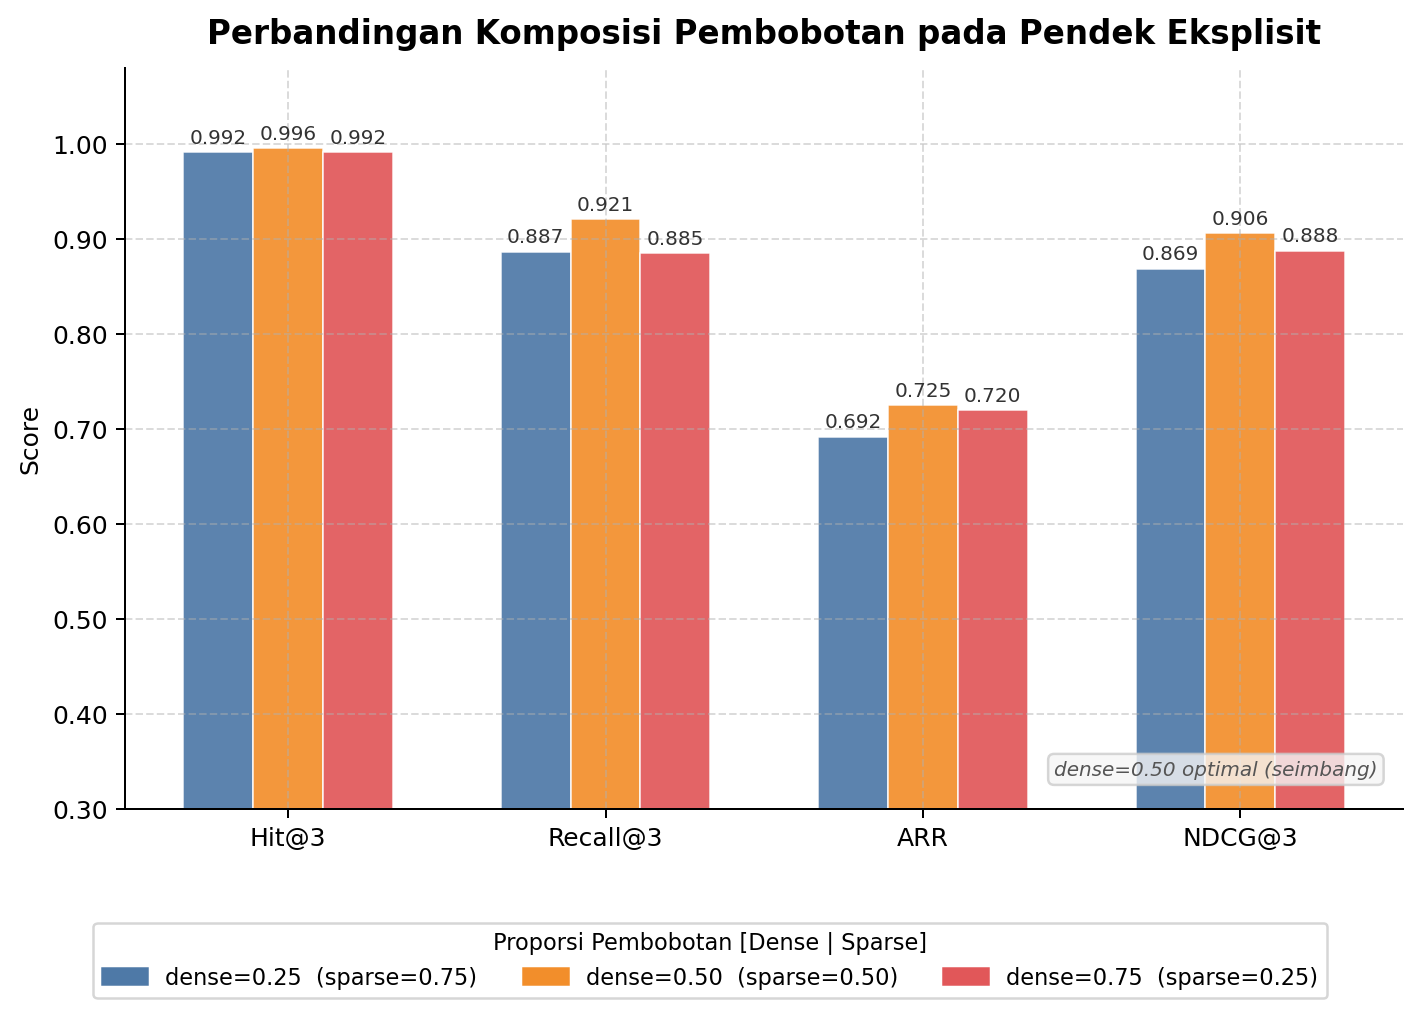
\includegraphics[width=0.85\textwidth]{Gambar/4.2.1.1/viz_A_eksplisit_short.png}
	\caption{Perbandingan metrik evaluasi berdasarkan komposisi \textit{dense-sparse} pada \textit{query} pendek eksplisit}
	\label{fig:komposisi_eksplisit_short}
\end{figure}

\textbf{Hasil pada \textit{Query} Panjang Eksplisit}

Komposisi dominan \textit{sparse} memberikan hasil lebih unggul pada metrik \textit{coverage}, dengan Hit@3 lebih tinggi 0.044 dan Recall@3 lebih tinggi 0.050 dibanding dominan \textit{dense}. Pada metrik \textit{rank-sensitive}, perbedaannya lebih kecil, tetapi dominan \textit{sparse} tetap sedikit lebih baik pada NDCG@3 sebesar 0.019, sedangkan ARR relatif setara. Hal ini menunjukkan bahwa \textit{query} eksplisit panjang lebih terbantu oleh pencocokan leksikal/\textit{sparse}.

\begin{figure}[H]
	\centering
	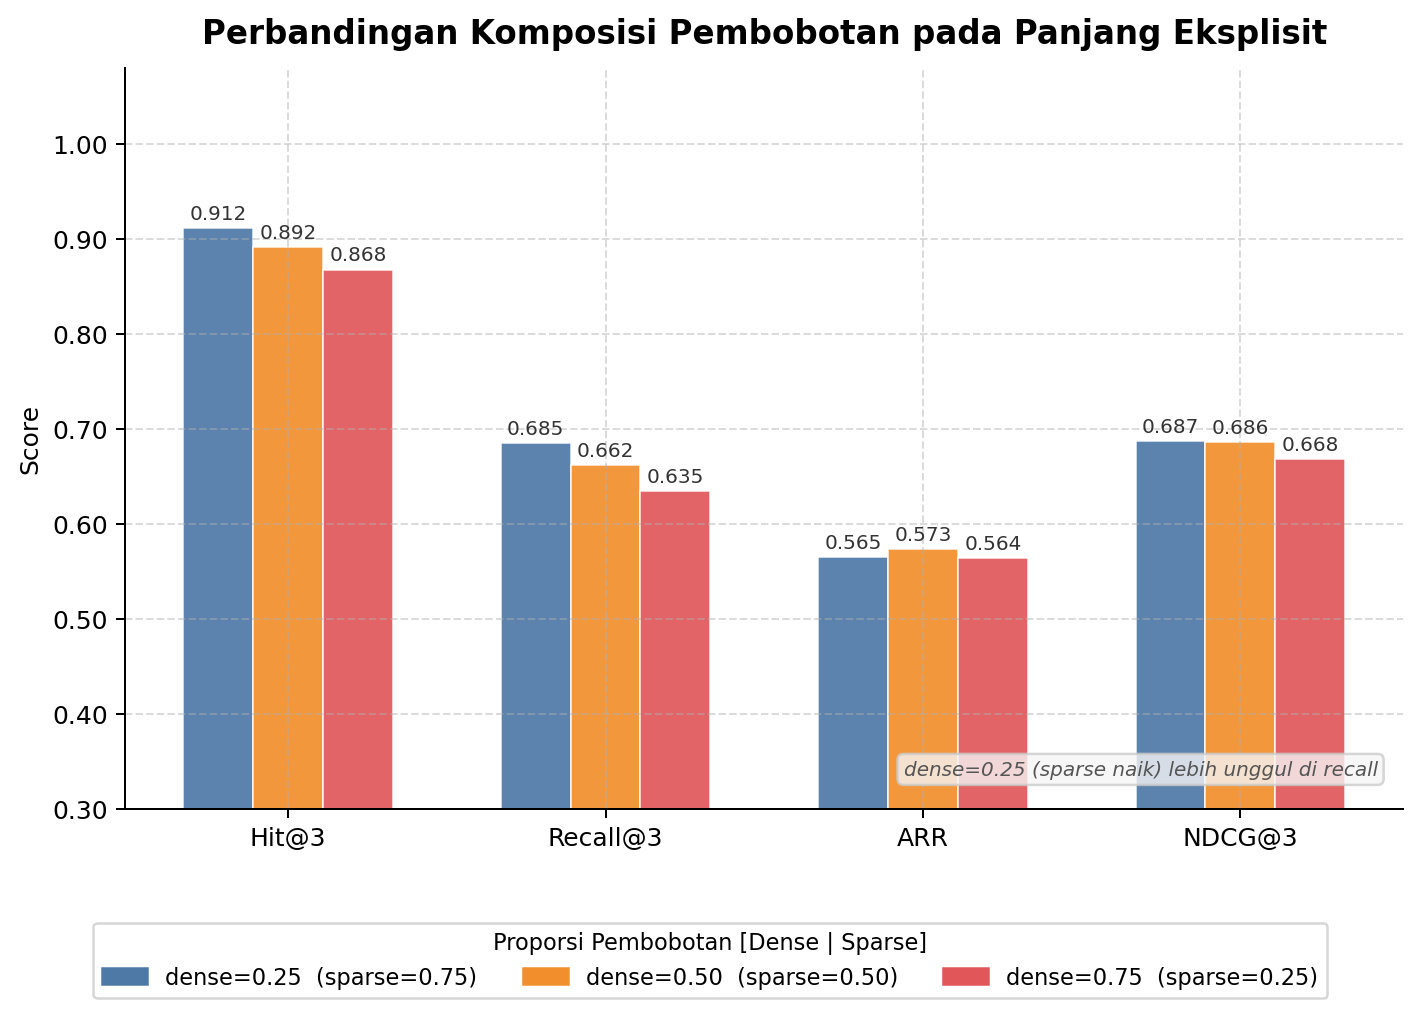
\includegraphics[width=0.85\textwidth]{Gambar/4.2.1.1/viz_A_eksplisit_long.png}
	\caption{Perbandingan metrik evaluasi berdasarkan komposisi \textit{dense-sparse} pada \textit{query} panjang eksplisit}
	\label{fig:komposisi_eksplisit_long}
\end{figure}

\textbf{Hasil pada \textit{Query} Pendek Implisit}

Komposisi seimbang 0.5:0.5 menjadi pembobotan terbaik pada seluruh metrik. Jika dibandingkan antara dominan \textit{sparse} dan dominan \textit{dense}, dominan \textit{sparse} sedikit lebih unggul, terutama pada ARR sebesar 0.015 dan NDCG@3 sebesar 0.013. Namun, peningkatan terbesar tetap diperoleh ketika \textit{dense} dan \textit{sparse} dikombinasikan secara seimbang.

\begin{figure}[H]
	\centering
	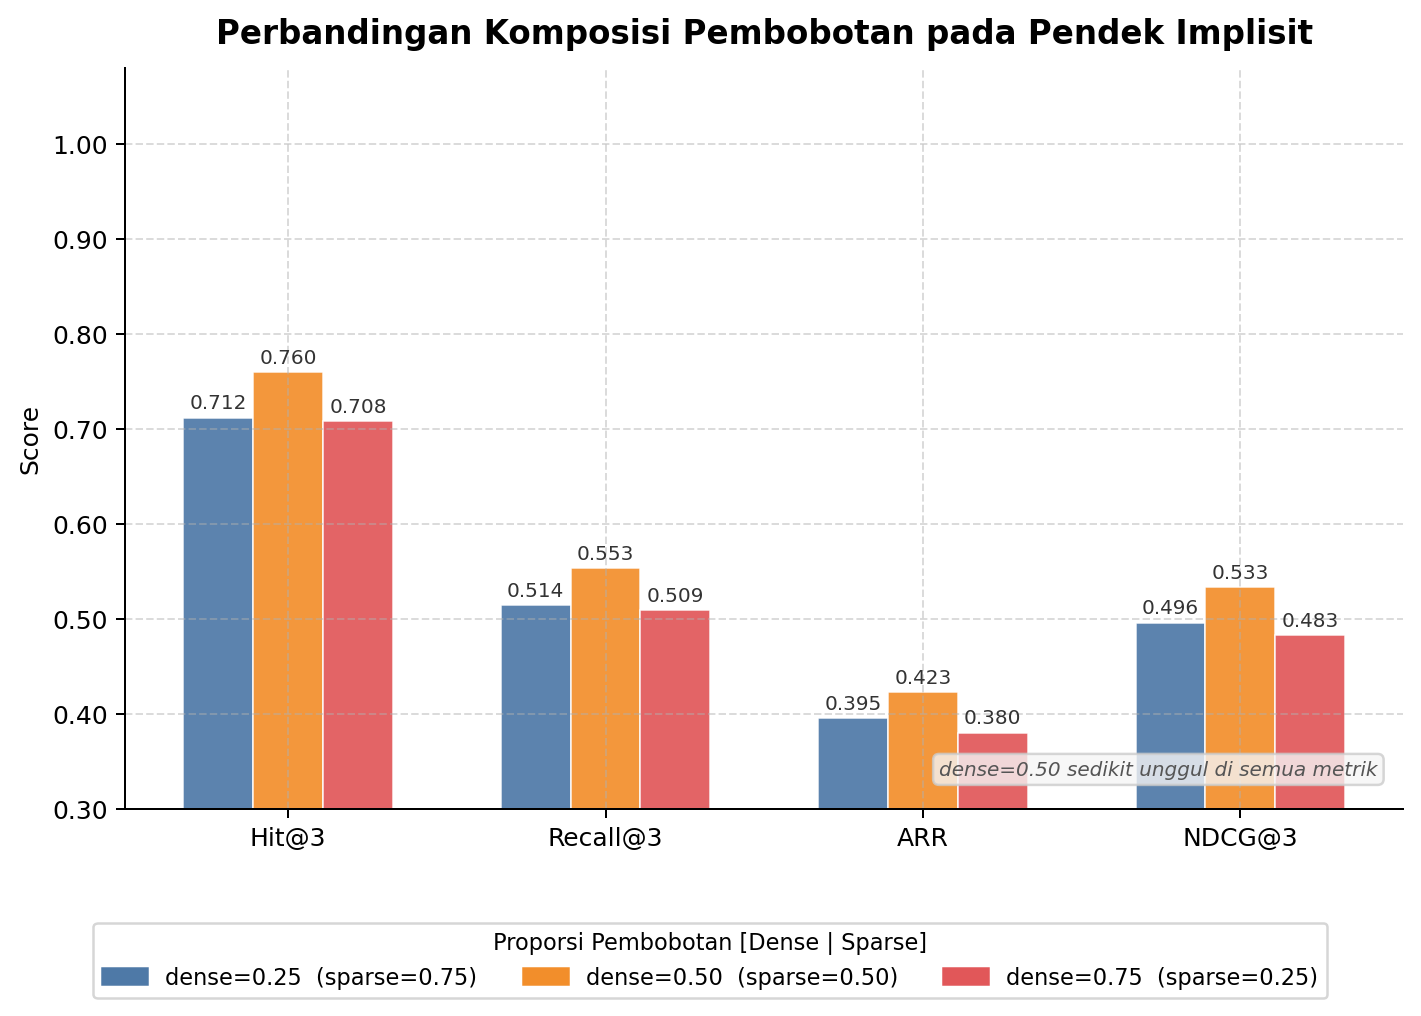
\includegraphics[width=0.85\textwidth]{Gambar/4.2.1.1/viz_A_implisit_short.png}
	\caption{Perbandingan metrik evaluasi berdasarkan komposisi \textit{dense-sparse} pada \textit{query} pendek implisit}
	\label{fig:komposisi_implisit_short}
\end{figure}

\textbf{Hasil pada \textit{Query} Panjang Implisit}

Komposisi seimbang 0.5:0.5 kembali menghasilkan performa terbaik pada seluruh metrik. Dominan \textit{sparse} juga lebih baik dibanding dominan \textit{dense}, dengan selisih Hit@3 sebesar 0.056, Recall@3 sebesar 0.052, ARR sebesar 0.045, dan NDCG@3 sebesar 0.058. Hasil ini menunjukkan bahwa dominasi \textit{dense} kurang optimal untuk \textit{query} implisit panjang, sementara kombinasi seimbang mampu menjaga cakupan sekaligus kualitas peringkat.

\begin{figure}[H]
	\centering
	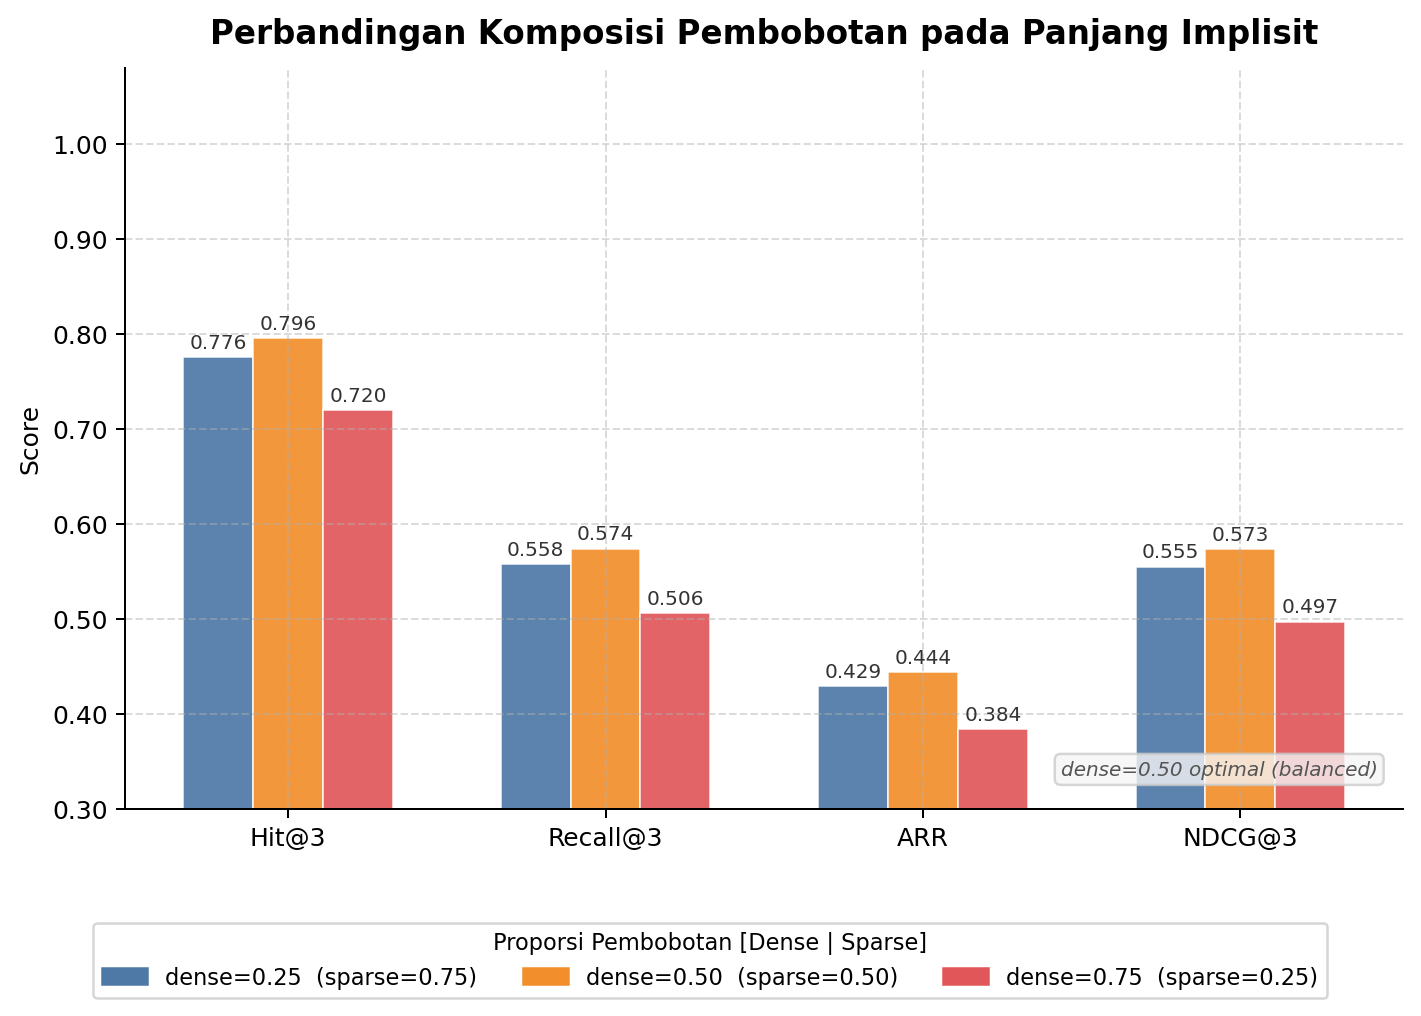
\includegraphics[width=0.85\textwidth]{Gambar/4.2.1.1/viz_A_implisit_long.png}
	\caption{Perbandingan metrik evaluasi berdasarkan komposisi \textit{dense-sparse} pada \textit{query} panjang implisit}
	\label{fig:komposisi_implisit_long}
\end{figure}

\subsubsection{Analisis Komparatif Jumlah \textit{Candidate Pool} pada \textit{Reranking Retrieval}}

\textbf{Hasil pada \textit{Query} Pendek Eksplisit}

\textit{Candidate pool} dengan ukuran terkecil, yaitu 5, konsisten memberikan nilai terbaik pada seluruh metrik dibanding \textit{pool} yang lebih besar. Metrik \textit{coverage} menunjukkan perbedaan kecil (Hit@3 = 0.004, Recall@3 = 0.014), sedangkan pada metrik \textit{rank-sensitive}, \textit{pool} 5 lebih unggul signifikan dengan ARR lebih tinggi 0.011 dan NDCG@3 lebih tinggi 0.013 dibanding \textit{pool} 10 hingga 20. \textit{Pool} 10, 15, dan 20 menghasilkan nilai yang hampir identik, sehingga penambahan kandidat di atas 10 tidak memberikan perbaikan.

\textbf{Hasil pada \textit{Query} Panjang Eksplisit}

\textit{Pool} 15 menjadi konfigurasi terbaik dengan unggul pada Hit@3 (0.968) dan ARR (0.582). Pola yang menarik adalah peningkatan kandidat dari \textit{pool} 5 ke 15 meningkatkan performa secara bertahap, namun \textit{pool} 20 justru menurun pada semua metrik. Penurunan ini menunjukkan bahwa terlalu banyak kandidat justru menurunkan kualitas \textit{reranking} pada \textit{query} eksplisit panjang, di mana \textit{noise} dari kandidat tambahan melemahkan akurasi peringkat.

\textbf{Hasil pada \textit{Query} Pendek Implisit}

\textit{Pool} 5 kembali memberikan performa terbaik pada seluruh metrik, dengan keunggulan yang lebih konsisten. Hit@3 lebih tinggi 0.032, Recall@3 lebih tinggi 0.048, ARR lebih tinggi 0.020, dan NDCG@3 lebih tinggi 0.031 dibanding \textit{pool} 20. Terlihat tren penurunan yang jelas seiring penambahan ukuran \textit{pool}, rata-rata penurunan konsisten terjadi pada setiap kenaikan \textit{step pool} (+5), yaitu Hit@3 turun rata-rata 0.019, Recall@3 turun 0.024, ARR turun 0.012, dan NDCG@3 turun 0.017 per \textit{step}. Hasil ini mengindikasikan bahwa \textit{query} implisit pendek sangat sensitif terhadap \textit{noise} dari kandidat tambahan.

\textbf{Hasil pada \textit{Query} Panjang Implisit}

\textit{Pool} 5 secara dominan mengungguli semua konfigurasi \textit{pool} lainnya pada seluruh metrik, dengan selisih yang paling besar dibanding tiga jenis \textit{query} sebelumnya. Hit@3 lebih tinggi 0.100, Recall@3 lebih tinggi 0.126, ARR lebih tinggi 0.094, dan NDCG@3 lebih tinggi 0.122 dibanding \textit{pool} 20. Rata-rata penurunan konsisten terjadi pada setiap kenaikan \textit{step pool} (+5), yaitu Hit@3 turun rata-rata 0.033, Recall@3 turun 0.042, ARR turun 0.031, dan NDCG@3 turun 0.041 per \textit{step}. Tren penurunan monoton yang tajam dari \textit{pool} 5 hingga \textit{pool} 20 menunjukkan bahwa \textit{query} implisit panjang sangat rentan terhadap degradasi akibat penambahan kandidat yang kurang relevan.

\begin{figure}[H]
	\centering
	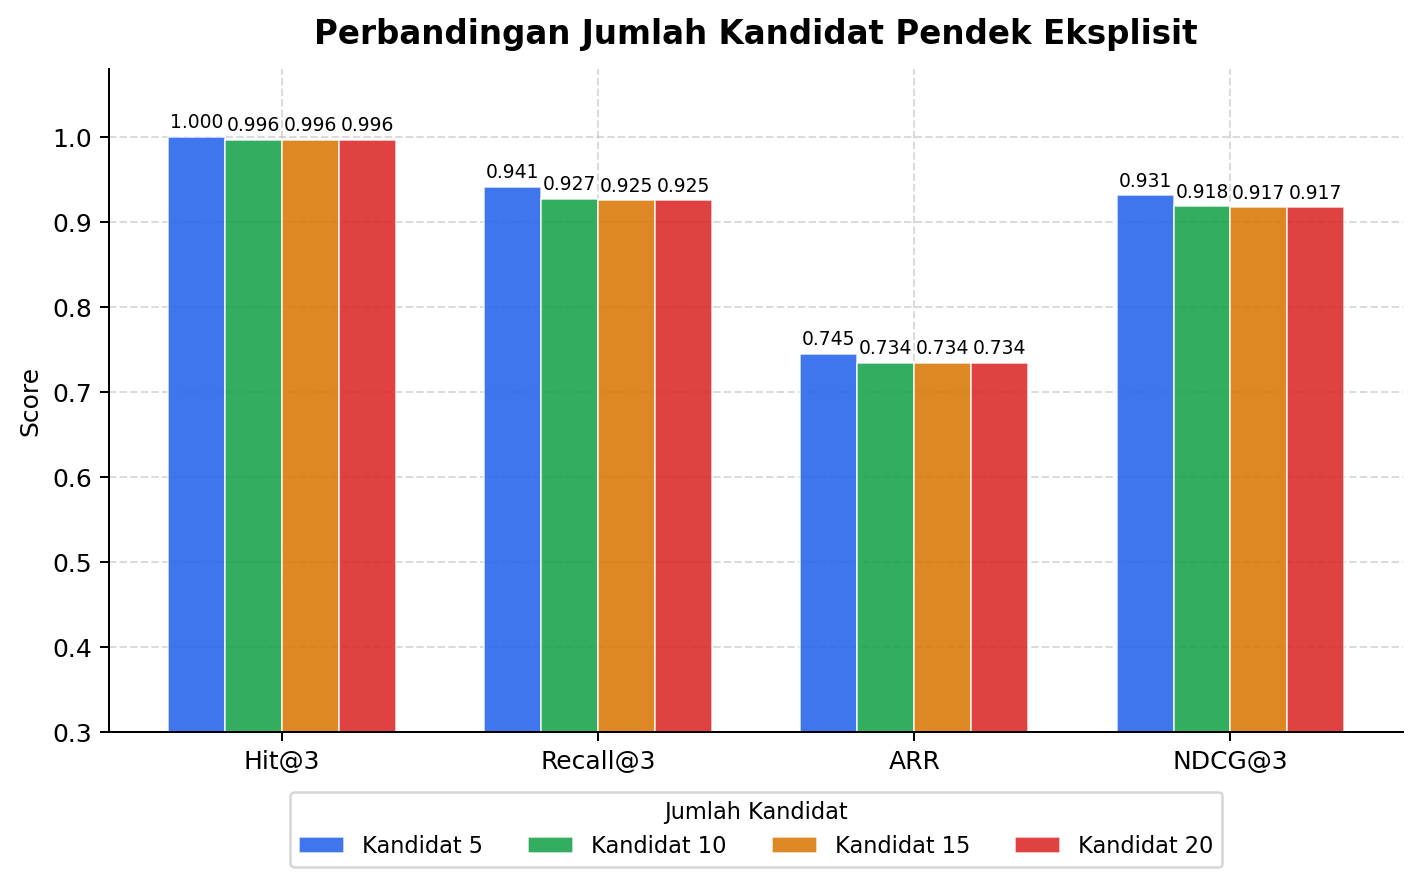
\includegraphics[width=0.85\textwidth]{Gambar/4.2.1.2/viz_optionA_eksplisit_short.png}
	\caption{Perbandingan metrik evaluasi berdasarkan ukuran \textit{candidate pool} pada \textit{query} pendek eksplisit}
	\label{fig:pool_eksplisit_short}
\end{figure}

\begin{figure}[H]
	\centering
	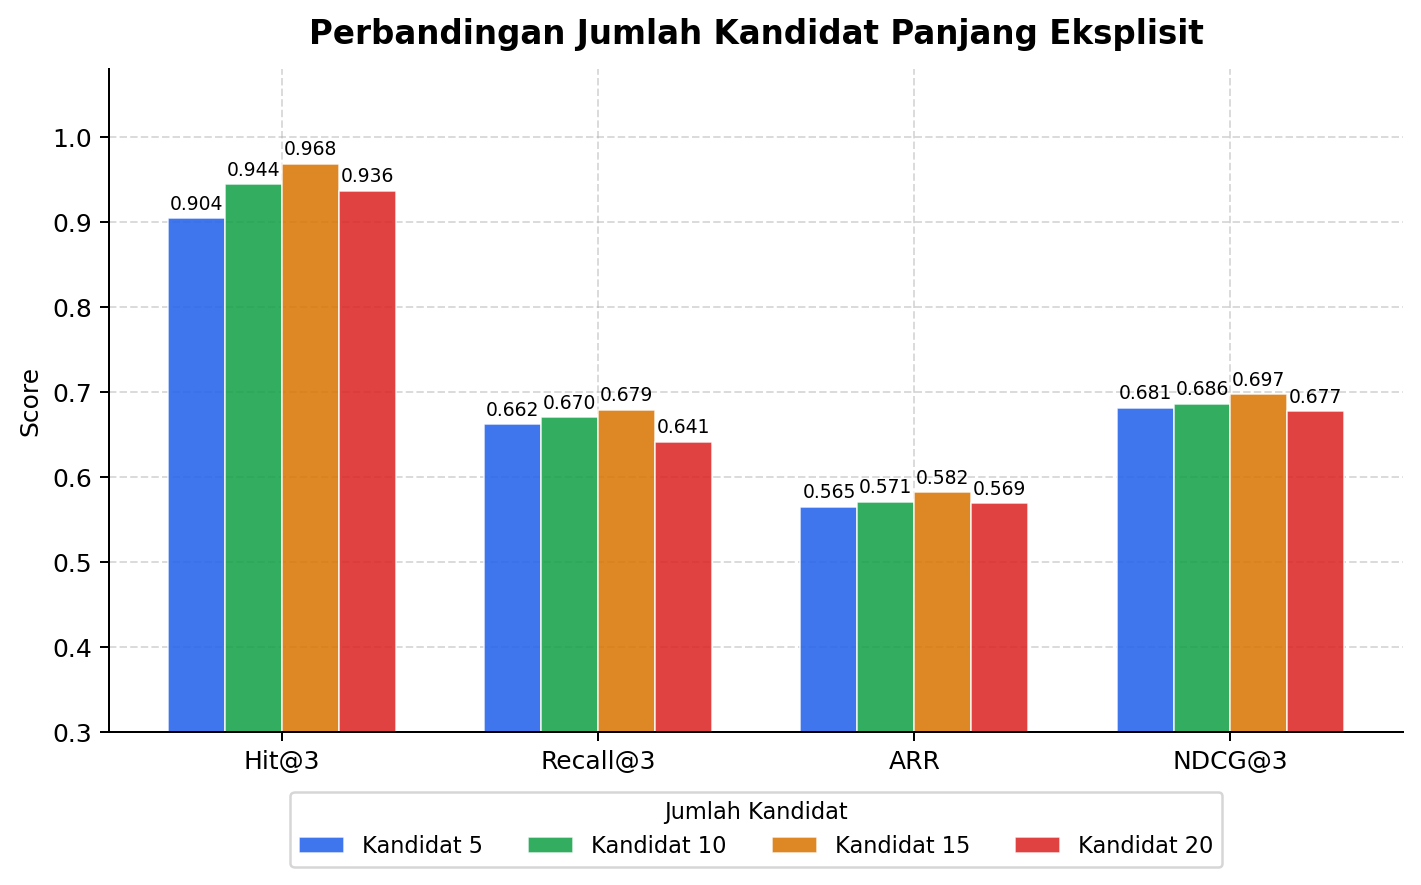
\includegraphics[width=0.85\textwidth]{Gambar/4.2.1.2/viz_optionA_eksplisit_long.png}
	\caption{Perbandingan metrik evaluasi berdasarkan ukuran \textit{candidate pool} pada \textit{query} panjang eksplisit}
	\label{fig:pool_eksplisit_long}
\end{figure}

\begin{figure}[H]
	\centering
	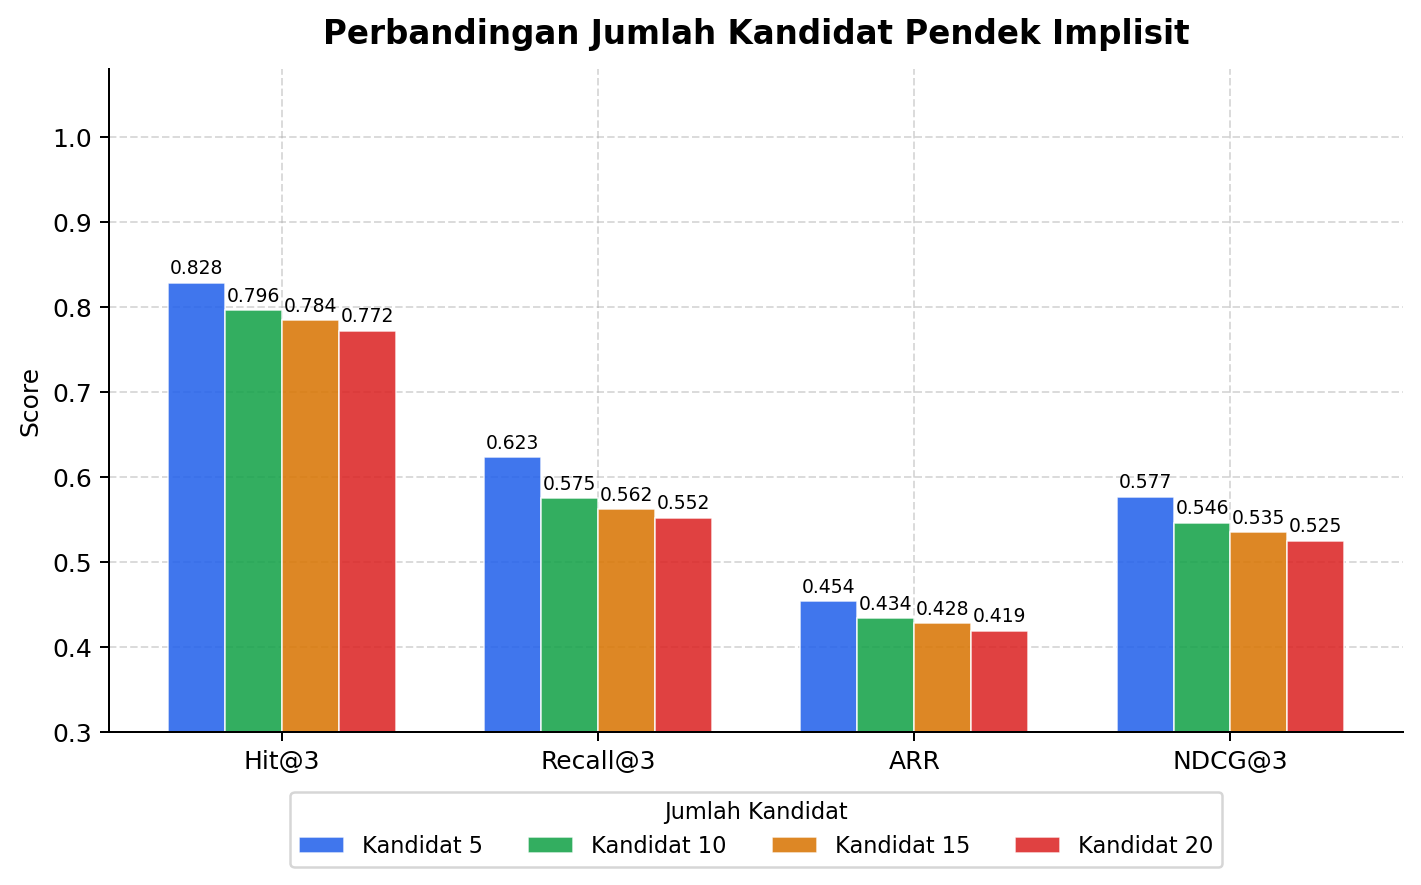
\includegraphics[width=0.85\textwidth]{Gambar/4.2.1.2/viz_optionA_implisit_short.png}
	\caption{Perbandingan metrik evaluasi berdasarkan ukuran \textit{candidate pool} pada \textit{query} pendek implisit}
	\label{fig:pool_implisit_short}
\end{figure}

\begin{figure}[H]
	\centering
	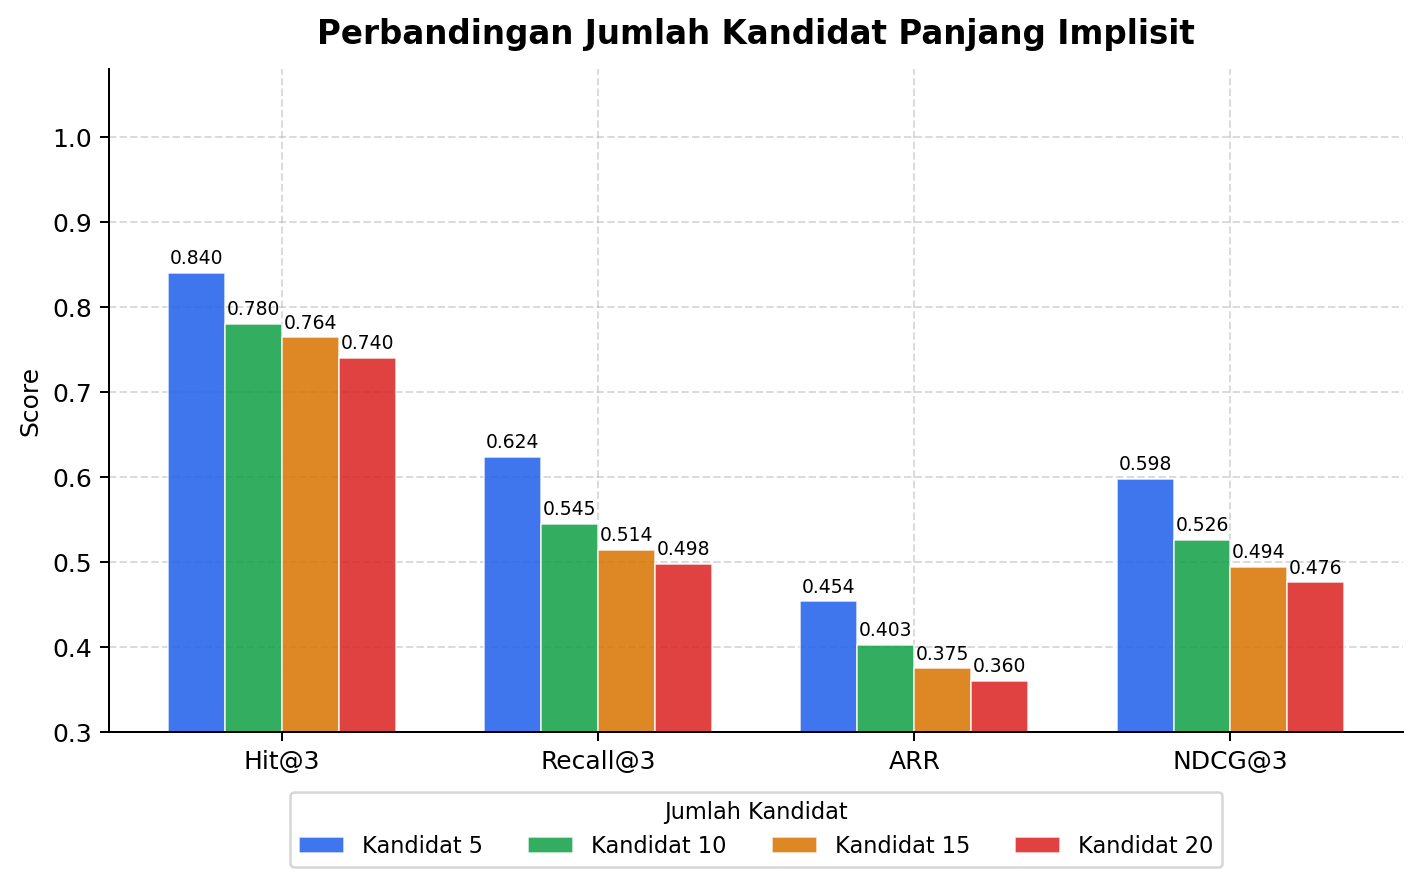
\includegraphics[width=0.85\textwidth]{Gambar/4.2.1.2/viz_optionA_implisit_long.png}
	\caption{Perbandingan metrik evaluasi berdasarkan ukuran \textit{candidate pool} pada \textit{query} panjang implisit}
	\label{fig:pool_implisit_long}
\end{figure}

\textbf{Hasil Waktu Latensi}

Berdasarkan rata-rata seluruh jenis \textit{query}, \textit{pool} 5 membutuhkan waktu 8.04 detik, \textit{pool} 10 meningkat menjadi 17.52 detik, \textit{pool} 15 menjadi 27.41 detik, dan \textit{pool} 20 mencapai 35.17 detik. Setiap penambahan 5 kandidat meningkatkan waktu rata-rata sekitar 9.49 detik dari \textit{pool} 5 ke 10, 9.89 detik dari \textit{pool} 10 ke 15, dan 7.75 detik dari \textit{pool} 15 ke 20. Hal ini menunjukkan bahwa semakin besar \textit{candidate pool}, semakin tinggi beban waktu proses \textit{reranking}.

\begin{figure}[H]
	\centering
	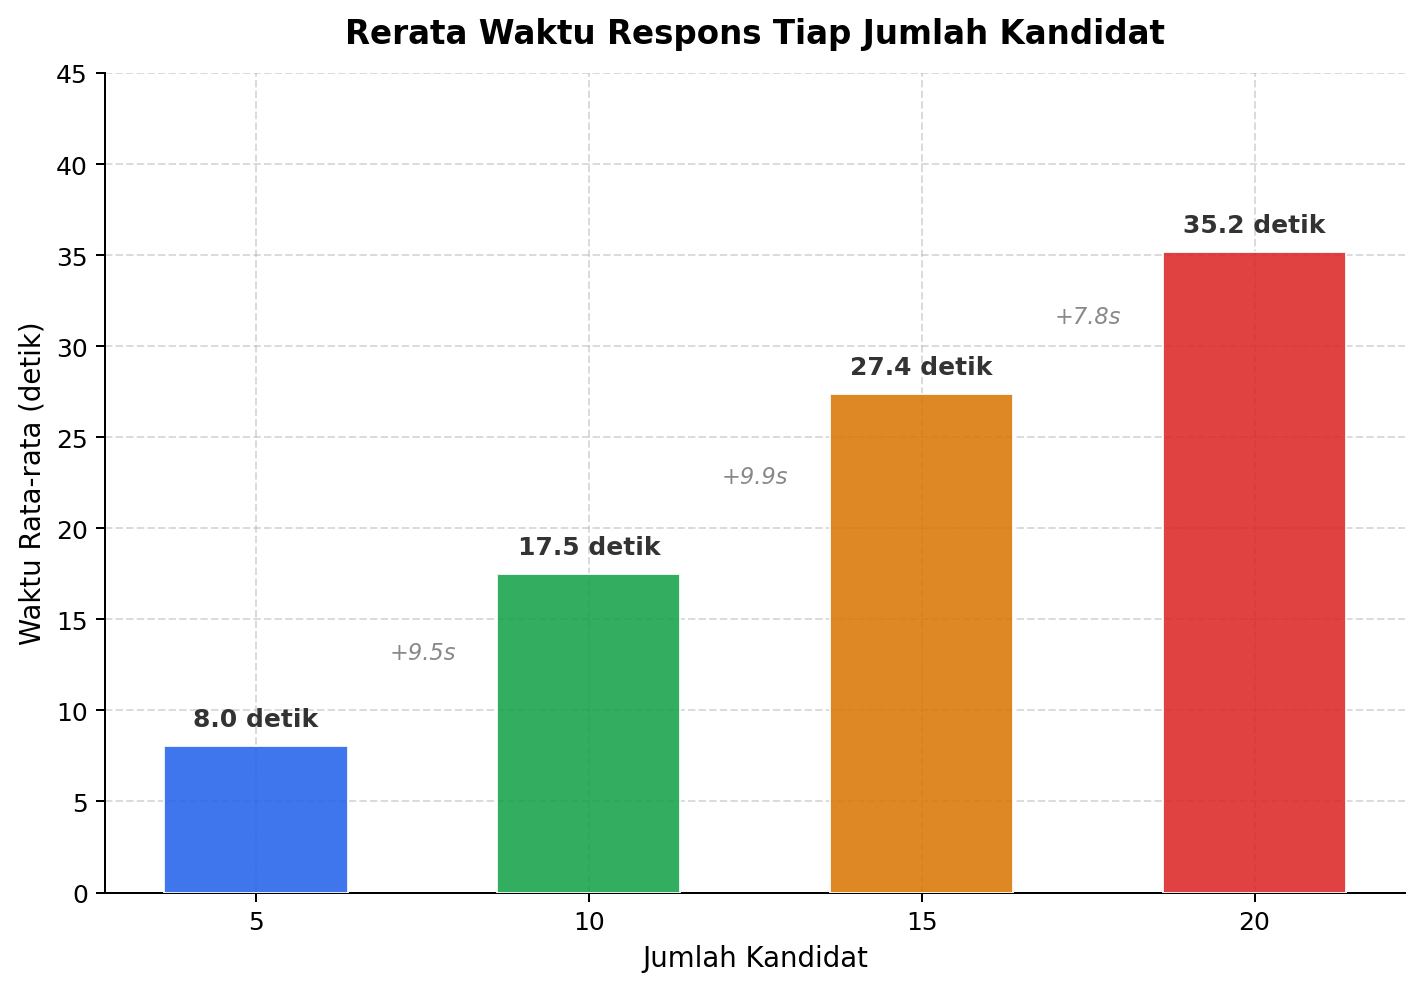
\includegraphics[width=0.85\textwidth]{Gambar/4.2.1.2/viz_time_per_pool.png}
	\caption{Perbandingan waktu latensi rata-rata berdasarkan ukuran \textit{candidate pool}}
	\label{fig:latensi_pool}
\end{figure}

\subsubsection{Analisis Komparatif Independen antara \textit{Hybrid Retrieval} dan \textit{Reranking}}

Perbandingan ini mengacu pada konfigurasi CE=0 (\textit{hybrid retrieval} dengan komposisi optimal 0.5:0.5) dan CE=1 (\textit{reranking retrieval} dengan \textit{pool} optimal 5). Secara umum, \textit{reranker} lebih unggul dibandingkan \textit{hybrid retrieval} pada sebagian besar jenis \textit{query}.

\textbf{Hasil pada \textit{Query} Pendek Eksplisit}

Metode \textit{Reranking} optimal dengan \textit{pool} 5 konsisten menghasilkan nilai terbaik pada seluruh metrik dibanding \textit{Hybrid Scoring} optimal komposisi 0.5:0.5. Keunggulan paling terlihat pada Recall@3 dan metrik \textit{rank-sensitive}, dengan Recall@3 lebih tinggi 0.020, ARR lebih tinggi 0.020, dan NDCG@3 lebih tinggi 0.025. Pada Hit@3, selisihnya relatif kecil yaitu 0.004, karena kedua metode sama-sama sudah mencapai cakupan yang sangat tinggi.

\textbf{Hasil pada \textit{Query} Panjang Eksplisit}

Performa \textit{Hybrid} dan \textit{Reranker} relatif seimbang pada \textit{query} eksplisit panjang. \textit{Reranker} sedikit lebih unggul pada Hit@3 sebesar 0.012, sedangkan Recall@3 menghasilkan nilai yang sama. Namun, pada metrik \textit{rank-sensitive}, \textit{Hybrid} sedikit lebih baik dengan ARR lebih tinggi 0.008 dan NDCG@3 lebih tinggi 0.005. Hal ini menunjukkan bahwa untuk \textit{query} eksplisit panjang, \textit{Hybrid} masih kompetitif dalam menjaga kualitas urutan dokumen.

\textbf{Hasil pada \textit{Query} Pendek Implisit}

\textit{Reranker pool} 5 memberikan peningkatan paling konsisten dibanding \textit{Hybrid} pada seluruh metrik. Selisih terbesar muncul pada metrik \textit{coverage}, yaitu Hit@3 lebih tinggi 0.068 dan Recall@3 lebih tinggi 0.070. Pada metrik \textit{rank-sensitive}, \textit{Reranker} juga unggul dengan ARR lebih tinggi 0.031 dan NDCG@3 lebih tinggi 0.044. Hasil ini menunjukkan bahwa \textit{reranking} membantu memperbaiki relevansi pada \textit{query} implisit pendek.

\textbf{Hasil pada \textit{Query} Panjang Implisit}

\textit{Reranker} kembali unggul pada seluruh metrik untuk \textit{query} implisit panjang. Dibanding \textit{Hybrid}, \textit{Reranker} meningkatkan Hit@3 sebesar 0.044 dan Recall@3 sebesar 0.050, sedangkan pada metrik \textit{rank-sensitive} ARR meningkat 0.010 dan NDCG@3 meningkat 0.025. Dengan demikian, \textit{Reranker} lebih efektif untuk \textit{query} implisit karena mampu menyaring kandidat yang lebih relevan setelah proses \textit{retrieval} awal.

\subsubsection{Analisis Komparatif Komposisi \textit{Scoring Hybrid Retrieval} dan \textit{Reranking}}

\textbf{Hasil pada \textit{Query} Pendek Eksplisit}

Komposisi dominan CE memberikan hasil lebih unggul pada metrik \textit{coverage}, dengan Recall@3 lebih tinggi 0.011 dibanding dominan \textit{Hybrid}, sedangkan Hit@3 relatif setara karena seluruh konfigurasi mencapai nilai 1.000. Pada metrik \textit{rank-sensitive}, dominan CE juga konsisten lebih baik, dengan ARR lebih tinggi 0.021 dan NDCG@3 lebih tinggi 0.021. Hal ini menunjukkan bahwa \textit{query} eksplisit pendek lebih terbantu oleh dominasi \textit{Cross-Encoder} dalam proses \textit{score fusion}.

\textbf{Hasil pada \textit{Query} Panjang Eksplisit}

Komposisi dominan \textit{Hybrid} memberikan hasil lebih unggul pada metrik \textit{coverage}, dengan Hit@3 lebih tinggi 0.004 dan Recall@3 lebih tinggi 0.015 dibanding dominan CE. Pada metrik \textit{rank-sensitive}, perbedaannya relatif kecil, di mana dominan CE sedikit lebih baik pada ARR sebesar 0.002, sedangkan dominan \textit{Hybrid} lebih unggul pada NDCG@3 sebesar 0.004. Namun, komposisi seimbang CE=0.50 menghasilkan ARR dan NDCG@3 terbaik, sehingga \textit{query} eksplisit panjang lebih optimal ketika bobot CE dan \textit{Hybrid} tidak terlalu dominan pada salah satu sisi.

\textbf{Hasil pada \textit{Query} Pendek Implisit}

Pada \textit{query} pendek implisit, konfigurasi dengan CE dominan (0.75) menghasilkan performa yang lebih baik pada metrik \textit{coverage}, sedangkan konfigurasi \textit{Hybrid} dominan lebih unggul pada metrik \textit{rank-sensitive}. Komposisi seimbang 0.5:0.5 kembali menjadi titik \textit{trade-off} yang optimal di antara keduanya.

\textbf{Hasil pada \textit{Query} Panjang Implisit}

Selain Hit@3 yang hasilnya relatif setara, komposisi seimbang 0.5:0.5 konsisten menghasilkan nilai terbaik pada metrik lainnya. Dominan \textit{Hybrid} sedikit lebih unggul pada Recall@3, sedangkan dominan CE sedikit lebih baik pada ARR dan NDCG@3. Hal ini mengonfirmasi bahwa keseimbangan bobot antara \textit{Hybrid} dan CE menghasilkan performa yang paling stabil pada \textit{query} implisit panjang.

\subsection{Analisis Hasil Eksperimen \textit{Query} Dokumen DTI}

\subsubsection{Analisis Komparatif Komposisi \textit{Dense} dan \textit{Sparse} pada \textit{Hybrid Retrieval}}

Sama seperti pada \textit{query} sintetis, proporsi 0.5:0.5 menjadi konfigurasi paling optimal untuk seluruh metrik kecuali Hit@3. Dominan \textit{sparse} selalu konsisten lebih baik dibanding dominan \textit{dense}, yang menunjukkan bahwa pencocokan leksikal tetap memiliki kontribusi penting pada dokumen DTI.

\subsubsection{Analisis Komparatif Jumlah \textit{Candidate Pool} pada \textit{Reranking Retrieval}}

Sama seperti pada \textit{query} sintetis, semakin banyak \textit{candidate pool} maka hasil akurasi menurun secara konsisten untuk keempat metrik evaluasi. \textit{Pool} 5 tetap menjadi konfigurasi terbaik yang meminimalkan \textit{noise} dan latensi tambahan.

\subsubsection{Analisis Komparatif Independen antara \textit{Hybrid Retrieval} dan \textit{Reranking}}

Berbeda dari \textit{query} sintetis yang lebih menguntungkan \textit{reranker}, pada kasus dokumen DTI komponen \textit{hybrid} lebih dominan dan menunjukkan performa yang lebih baik. Hal ini mengindikasikan bahwa karakteristik \textit{query} dari dokumen nyata DTI lebih sesuai dengan pendekatan \textit{hybrid retrieval} dibandingkan \textit{reranking} murni.

\subsubsection{Analisis Komparatif Komposisi \textit{Scoring Hybrid Retrieval} dan \textit{Reranking}}

Sejalan dengan hasil analisis independen, pada kasus dokumen DTI komponen \textit{hybrid} lebih dominan dalam proses \textit{score fusion}. Hal ini berbeda dengan pola pada \textit{query} sintetis yang lebih diuntungkan dengan dominasi \textit{Cross-Encoder}.

\cleardoublepage \phantomsection
\chapter{Kesimpulan dan Saran}

\section{Kesimpulan}

Berdasarkan hasil penelitian dan pembahasan pada Bab~4 mengenai evaluasi strategi \textit{retrieval} dalam sistem \textit{Retrieval-Augmented Generation} (RAG) untuk pemetaan kontrol \textit{Statement of Applicability} (SoA) ISO/IEC 27001:2022, dapat ditarik kesimpulan sebagai berikut.

\begin{enumerate}
	\item \textit{Hybrid retrieval} dengan proporsi \textit{dense}=0,50:\textit{sparse}=0,50 menghasilkan performa terbaik pada Recall@3=0,537, MAP@3=0,467, dan NDCG@3=0,575. Perbedaan performa antar konfigurasi terbukti signifikan secara statistik ($p < 0{,}001$), yang mengonfirmasi bahwa pemetaan kontrol ISO 27001 membutuhkan kombinasi pencocokan semantik dan leksikal.

	\item \textit{Candidate pool} berukuran 5 menghasilkan performa terbaik pada seluruh metrik (Hit@3=0,857, Recall@3=0,468, MAP@3=0,387, NDCG@3=0,485) dengan latensi terendah (5,91 detik). Penambahan ukuran \textit{pool} justru menurunkan performa secara monoton karena memperbanyak kandidat yang kurang relevan pada tahap \textit{reranking} ($p < 0{,}003$).

	\item \textit{Score fusion} dengan proporsi Hybrid:CE=0,75:0,25 menghasilkan performa terbaik secara keseluruhan (Recall@3=0,541, MAP@3=0,470, NDCG@3=0,579). \textit{Hybrid retrieval} dan \textit{cross-encoder} bersifat komplementer: \textit{hybrid} unggul pada \textit{query} dengan terminologi teknis spesifik (36 dari 77 \textit{query}), sementara \textit{cross-encoder} memberikan nilai tambah pada \textit{query} yang membutuhkan pemahaman kontekstual (15 dari 77 \textit{query}).
\end{enumerate}

Secara keseluruhan, konfigurasi optimal yang teridentifikasi adalah \textit{hybrid retrieval} dengan proporsi \textit{dense}=0,50:\textit{sparse}=0,50, \textit{candidate pool} berukuran 5, dan \textit{score fusion} dengan proporsi Hybrid:CE=0,75:0,25, yang mencapai keseimbangan terbaik antara kualitas \textit{retrieval} dan efisiensi komputasi.

\section{Saran}

Berdasarkan hasil penelitian yang telah dilakukan, beberapa saran untuk penelitian selanjutnya adalah sebagai berikut.

\begin{enumerate}
	\item \textbf{Evaluasi pada domain dan organisasi yang berbeda.} Konfigurasi optimal yang ditemukan perlu diuji pada dokumen kebijakan organisasi lain dengan karakteristik terminologi dan ruang lingkup kontrol yang berbeda untuk memvalidasi generalisasi temuan.

	\item \textbf{Eksplorasi granularitas parameter yang lebih spesifik.} Penelitian ini menguji pembobotan dengan kelipatan 0,25 pada tiga sumbu desain. Penelitian selanjutnya dapat menerapkan \textit{grid search} dengan resolusi lebih halus (kelipatan 0,05 atau 0,10), serta mengevaluasi metode \textit{reranking} alternatif seperti \textit{listwise reranker} atau model berbasis LLM.

	\item \textbf{Analisis granular pada domain kontrol yang kurang terwakili.} Dataset penelitian ini didominasi domain A.5 dan A.8 (96,5\%), sementara A.6 dan A.7 sangat terbatas. Penelitian selanjutnya perlu mengonstruksi dataset dengan cakupan lebih merata pada keempat domain untuk memvalidasi konsistensi konfigurasi optimal.

	\item \textbf{Evaluasi \textit{pipeline} RAG secara menyeluruh.} Penelitian selanjutnya perlu mengevaluasi \textit{pipeline} RAG secara \textit{end-to-end}, meliputi tahap \textit{pre-retrieval} (\textit{document chunking}), \textit{retrieval} dengan konfigurasi optimal, serta tahap \textit{generation} dengan LLM untuk mengevaluasi \textit{faithfulness} dan utilitas rekomendasi kontrol.

	\item \textbf{Validasi hasil oleh praktisi profesional bersertifikat.} Pemetaan manual kontrol Annex pada penelitian ini dilakukan oleh peneliti. Penelitian selanjutnya perlu melibatkan auditor bersertifikat ISO 27001 untuk memvalidasi akurasi \textit{ground truth} dan relevansi hasil pemetaan.

	\item \textbf{Penerapan uji \textit{post-hoc} untuk perbandingan berpasangan.} Penelitian ini menggunakan uji Friedman secara keseluruhan namun belum dilanjutkan uji \textit{post-hoc} seperti Wilcoxon dengan koreksi Bonferroni untuk mengidentifikasi pasangan konfigurasi mana yang benar-benar berbeda secara signifikan.

	\item \textbf{Klasifikasi otomatis jenis \textit{query} berdasarkan karakteristik \textit{retrieval}.} \textit{Hybrid retrieval} dan \textit{cross-encoder} bersifat komplementer bergantung pada karakteristik \textit{query}. Penelitian selanjutnya perlu mengembangkan skema klasifikasi \textit{query} dan mekanisme \textit{adaptive retrieval} yang menyesuaikan pembobotan secara dinamis per \textit{query}.

	\item \textbf{Eksplorasi desain basis pengetahuan dan pemilihan komponen model.} Penelitian selanjutnya perlu menguji variasi desain basis pengetahuan (struktur atribut, cakupan informasi, representasi teks) serta mengeksplorasi kombinasi komponen model (\textit{sparse retrieval}, \textit{dense embedding}, \textit{reranker}) yang lebih efektif pada domain pemetaan kontrol ISO/IEC 27001.
\end{enumerate}


\cleardoublepage \phantomsection
\bibliographystyle{IEEEtran}
\thereferences
\bibliography{references}

\end{document}
